%&preformat-disser
\RequirePackage[l2tabu,orthodox]{nag} % Раскомментировав, можно в логе получать рекомендации относительно правильного использования пакетов и предупреждения об устаревших и нерекомендуемых пакетах
% Формат А4, 14pt (ГОСТ Р 7.0.11-2011, 5.3.6)
\documentclass[a4paper,14pt,oneside,openany]{memoir}

%%%%%%%%%%%%%%%%%%%%%%%%%%%%%%%%%%%%%%%%%%%%%%%%%%%%%%%%%%%%%%%%%%%%%%%%%%%%%%%%
%%%% Файл упрощённых настроек шаблона, общих для диссертации и автореферата %%%%
%%%%%%%%%%%%%%%%%%%%%%%%%%%%%%%%%%%%%%%%%%%%%%%%%%%%%%%%%%%%%%%%%%%%%%%%%%%%%%%%

%%% Режим черновика %%%
\makeatletter
\@ifundefined{c@draft}{
  \newcounter{draft}
  \setcounter{draft}{1}  % 0 --- чистовик (максимальное соблюдение ГОСТ)
                         % 1 --- черновик (отклонения от ГОСТ, но быстрая
                         %       сборка итоговых PDF)
}{}
\makeatother

%%% Пометки в тексте %%%
\makeatletter
\@ifundefined{c@showmarkup}{
  \newcounter{showmarkup}
  \setcounter{showmarkup}{1}  % 0 --- скрыть пометки
                              % 1 --- показывать пометки
}{}
\makeatother

%%% Использование в pdflatex шрифтов не по-умолчанию %%%
\makeatletter
\@ifundefined{c@usealtfont}{
  \newcounter{usealtfont}
  \setcounter{usealtfont}{1}    % 0 --- шрифты на базе Computer Modern
                                % 1 --- использовать пакет pscyr, при его
                                %       наличии
                                % 2 --- использовать пакет XCharter, при наличии
                                %       подходящей версии
}{}
\makeatother

%%% Использование в xelatex и lualatex семейств шрифтов %%%
\makeatletter
\@ifundefined{c@fontfamily}{
  \newcounter{fontfamily}
  \setcounter{fontfamily}{1}  % 0 --- CMU семейство. Используется как fallback;
                              % 1 --- Шрифты от MS (Times New Roman и компания)
                              % 2 --- Семейство Liberation
}{}
\makeatother

%%% Библиография %%%
\makeatletter
\@ifundefined{c@bibliosel}{
  \newcounter{bibliosel}
  \setcounter{bibliosel}{1}   % 0 --- встроенная реализация с загрузкой файла
                              %       через движок bibtex8;
                              % 1 --- реализация пакетом biblatex через движок
                              %       biber
}{}
\makeatother

%%% Вывод типов ссылок в библиографии %%%
\makeatletter
\@ifundefined{c@mediadisplay}{
  \newcounter{mediadisplay}
  \setcounter{mediadisplay}{1}   % 0 --- не делать ничего; надписи [Текст] и
                                 %       [Эл. ресурс] будут выводиться только в ссылках с
                                 %       заполненным полем `media`;
                                 % 1 --- автоматически добавлять надпись [Текст] к ссылкам с
                                 %       незаполненным полем `media`; таким образом, у всех
                                 %       источников будет указан тип, что соответствует
                                 %       требованиям ГОСТ
                                 % 2 --- автоматически удалять надписи [Текст], [Эл. Ресурс] и др.;
                                 %       не соответствует ГОСТ
                                 % 3 --- автоматически удалять надпись [Текст];
                                 %       не соответствует ГОСТ
                                 % 4 --- автоматически удалять надпись [Эл. Ресурс];
                                 %       не соответствует ГОСТ
}{}
\makeatother

%%% Предкомпиляция tikz рисунков для ускорения работы %%%
\makeatletter
\@ifundefined{c@imgprecompile}{
  \newcounter{imgprecompile}
  \setcounter{imgprecompile}{0}   % 0 --- без предкомпиляции;
                                  % 1 --- пользоваться предварительно
                                  %       скомпилированными pdf вместо генерации
                                  %       заново из tikz
}{}
\makeatother
            % общие настройки шаблона
%%% Проверка используемого TeX-движка %%%
\newif\ifxetexorluatex   % определяем новый условный оператор (http://tex.stackexchange.com/a/47579)
\ifxetex
    \xetexorluatextrue
\else
    \ifluatex
        \xetexorluatextrue
    \else
        \xetexorluatexfalse
    \fi
\fi

\newif\ifsynopsis           % Условие, проверяющее, что документ --- автореферат

\usepackage{etoolbox}[2015/08/02]   % Для продвинутой проверки разных условий
\providebool{presentation}

\usepackage{comment}    % Позволяет убирать блоки текста (добавляет
                        % окружение comment и команду \excludecomment)

%%% Поля и разметка страницы %%%
\usepackage{pdflscape}  % Для включения альбомных страниц
\usepackage{geometry}   % Для последующего задания полей

%%% Математические пакеты %%%
\usepackage{amsthm,amsmath,amscd}   % Математические дополнения от AMS
\usepackage{amsfonts,amssymb}       % Математические дополнения от AMS
\usepackage{mathtools}              % Добавляет окружение multlined
\usepackage{xfrac}                  % Красивые дроби
\usepackage[
    locale = DE,
    list-separator       = {;\,},
    list-final-separator = {;\,},
    list-pair-separator  = {;\,},
    list-units           = single,
    range-units          = single,
    range-phrase={\text{\ensuremath{-}}},
    % quotient-mode        = fraction, % красивые дроби могут не соответствовать ГОСТ
    fraction-function    = \sfrac,
    separate-uncertainty,
    ]{siunitx}[=v2]                 % Размерности SI
\sisetup{inter-unit-product = \ensuremath{{}\cdot{}}}

% Кириллица в нумерации subequations
% Для правильной работы требуется выполнение сразу после загрузки пакетов
\patchcmd{\subequations}{\def\theequation{\theparentequation\alph{equation}}}
{\def\theequation{\theparentequation\asbuk{equation}}}
{\typeout{subequations patched}}{\typeout{subequations not patched}}

%%%% Установки для размера шрифта 14 pt %%%%
%% Формирование переменных и констант для сравнения (один раз для всех подключаемых файлов)%%
%% должно располагаться до вызова пакета fontspec или polyglossia, потому что они сбивают его работу
\newlength{\curtextsize}
\newlength{\bigtextsize}
\setlength{\bigtextsize}{13.9pt}

\makeatletter
%\show\f@size    % неплохо для отслеживания, но вызывает стопорение процесса,
                 % если документ компилируется без команды  -interaction=nonstopmode
\setlength{\curtextsize}{\f@size pt}
\makeatother

%%% Кодировки и шрифты %%%
\ifxetexorluatex
    \ifpresentation
        \providecommand*\autodot{} % quick fix for polyglossia 1.50
    \fi
    \PassOptionsToPackage{no-math}{fontspec}    % https://tex.stackexchange.com/a/26295/104425
    \usepackage{polyglossia}[2014/05/21]        % Поддержка многоязычности
                                        % (fontspec подгружается автоматически)
\else
   %%% Решение проблемы копирования текста в буфер кракозябрами
    \ifnumequal{\value{usealtfont}}{0}{}{
        \input glyphtounicode.tex
        \input glyphtounicode-cmr.tex %from pdfx package
        \pdfgentounicode=1
    }
    \usepackage{cmap}   % Улучшенный поиск русских слов в полученном pdf-файле
    \ifnumequal{\value{usealtfont}}{2}{}{
        \defaulthyphenchar=127  % Если стоит до fontenc, то переносы
                                % не впишутся в выделяемый текст при
                                % копировании его в буфер обмена
    }
    \usepackage{textcomp}
    \usepackage[T1,T2A]{fontenc}                    % Поддержка русских букв
    \ifnumequal{\value{usealtfont}}{1}{% Используется pscyr, при наличии
        \IfFileExists{pscyr.sty}{\usepackage{pscyr}}{}  % Подключение pscyr
    }{}
    \usepackage[utf8]{inputenc}[2014/04/30]         % Кодировка utf8
    \usepackage[english, russian]{babel}[2014/03/24]% Языки: русский, английский
    \makeatletter\AtBeginDocument{\let\@elt\relax}\makeatother % babel 3.40 fix
    \ifnumequal{\value{usealtfont}}{2}{
        % http://dxdy.ru/post1238763.html#p1238763
        \usepackage[scaled=0.914]{XCharter}[2017/12/19] % Подключение русифицированных шрифтов XCharter
        \usepackage[charter, vvarbb, scaled=1.048]{newtxmath}[2017/12/14]
        \ifpresentation
        \else
            \setDisplayskipStretch{-0.078}
        \fi
    }{}
\fi

%%% Оформление абзацев %%%
\ifpresentation
\else
    \indentafterchapter     % Красная строка после заголовков типа chapter
    \usepackage{indentfirst}
\fi

%%% Цвета %%%
\ifpresentation
\else
    \usepackage[dvipsnames, table, hyperref]{xcolor} % Совместимо с tikz
\fi

%%% Таблицы %%%
\usepackage{longtable} % Длинные таблицы
\usepackage{multirow,makecell}   % Улучшенное форматирование таблиц
%\usepackage{tabulary,tabularray} % Таблицы с автоматически подбирающейся
                                 % шириной столбцов
%\UseTblrLibrary{booktabs}
\ExplSyntaxOn% define \IfTokenListEmpty to use \captionof with tabularray
\prg_generate_conditional_variant:Nnn \tl_if_empty:n { e } { TF }
\let \IfTokenListEmpty = \tl_if_empty:eTF
\ExplSyntaxOff

\usepackage{threeparttable}      % автоматический подгон ширины подписи таблицы

%%% Общее форматирование
%\usepackage{soul}% Поддержка переносоустойчивых подчёркиваний и зачёркиваний
\usepackage{icomma}  % Запятая в десятичных дробях

%%% Оптимизация расстановки переносов и длины последней строки абзаца
\IfFileExists{impnattypo.sty}{% проверка установленности пакета impnattypo
    \ifluatex
        \ifnumequal{\value{draft}}{1}{% Черновик
            \usepackage[hyphenation, lastparline, nosingleletter, homeoarchy,
            rivers, draft]{impnattypo}
        }{% Чистовик
            \usepackage[hyphenation, lastparline, nosingleletter]{impnattypo}
        }
    \else
        \usepackage[hyphenation, lastparline]{impnattypo}
    \fi
}{}

%% Векторная графика

\usepackage{tikz}                   % Продвинутый пакет векторной графики
\usetikzlibrary{chains}             % Для примера tikz рисунка
\usetikzlibrary{shapes.geometric}   % Для примера tikz рисунка
\usetikzlibrary{shapes.symbols}     % Для примера tikz рисунка
\usetikzlibrary{arrows}             % Для примера tikz рисунка

\usepackage[european,cuteinductors]{circuitikz} % Электрические схемы
\usepackage{pgfplots}                           % Графики
\pgfplotsset{compat=newest}
\usepgfplotslibrary{groupplots,units}
\pgfkeys{/pgf/number format/.cd,use comma,1000 sep={}} % форматирование чисел в графиках

%%% Гиперссылки %%%
\ifxetexorluatex
    \let\CYRDZE\relax
\fi
\usepackage{hyperref}[2012/11/06]

%%% Изображения %%%
\usepackage{graphicx}[2014/04/25]   % Подключаем пакет работы с графикой
\usepackage{caption}                % Подписи рисунков и таблиц
\usepackage{subcaption}             % Подписи подрисунков и подтаблиц
\usepackage{pdfpages}               % Добавление внешних pdf файлов

%%% Счётчики %%%
\usepackage{aliascnt}
\usepackage[figure,table]{totalcount}   % Счётчик рисунков и таблиц
\usepackage{totcount}   % Пакет создания счётчиков на основе последнего номера
                        % подсчитываемого элемента (может требовать дважды
                        % компилировать документ)
\usepackage{totpages}   % Счётчик страниц, совместимый с hyperref (ссылается
                        % на номер последней страницы). Желательно ставить
                        % последним пакетом в преамбуле

%%% Продвинутое управление групповыми ссылками (пока только формулами) %%%
\ifpresentation
\else
    \usepackage[russian]{cleveref} % cleveref имеет сложности со считыванием
    % языка из babel. Такое решение русификации вывода выбрано вместо
    % определения в documentclass из опасности что-то лишнее передать во все
    % остальные пакеты, включая библиографию.

    % Добавление возможности использования пробелов в \labelcref
    % https://tex.stackexchange.com/a/340502/104425
    \usepackage{kvsetkeys}
    \makeatletter
    \let\org@@cref\@cref
    \renewcommand*{\@cref}[2]{%
        \edef\process@me{%
            \noexpand\org@@cref{#1}{\zap@space#2 \@empty}%
        }\process@me
    }
    \makeatother
\fi

\usepackage{placeins} % для \FloatBarrier

\ifnumequal{\value{draft}}{1}{% Черновик
    \usepackage[firstpage]{draftwatermark}
    \SetWatermarkText{DRAFT}
    \SetWatermarkFontSize{14pt}
    \SetWatermarkScale{15}
    \SetWatermarkAngle{45}
}{}

%%% Цитата, не приводимая в автореферате:
% возможно, актуальна только для biblatex
%\newcommand{\insynopsis}[1]{\ifsynopsis\else ~\cite{#1} \fi}

% если текущий процесс запущен библиотекой tikz-external, то прекомпиляция должна быть включена
\ifdefined\tikzexternalrealjob
    \setcounter{imgprecompile}{1}
\fi

\ifnumequal{\value{imgprecompile}}{1}{% Только если у нас включена предкомпиляция
    \usetikzlibrary{external}   % подключение возможности предкомпиляции
    \tikzexternalize[prefix=images/cache/,optimize command away=\includepdf] % activate! % здесь можно указать отдельную папку для скомпилированных файлов
    \ifxetex
        \tikzset{external/up to date check={diff}}
    \fi
}{}
         % Пакеты общие для диссертации и автореферата
\synopsisfalse                      % Этот документ --- не автореферат
%%% Прикладные пакеты %%%
%\usepackage{calc}               % Пакет для расчётов параметров, например длины

%%% Для добавления Стр. над номерами страниц в оглавлении
%%% http://tex.stackexchange.com/a/306950
\usepackage{afterpage}

%%% Списки %%%
\usepackage{enumitem}

%%% Оформление списка обозначений
\usepackage[intoc]{nomencl}
\makenomenclature
\setlength{\nomitemsep}{-.8\parsep}
    % Пакеты для диссертации
\usepackage{fr-longtable}    %ради \endlasthead

% Листинги с исходным кодом программ
\usepackage{fancyvrb}
\usepackage{listings}
\lccode`\~=0\relax %Без этого хака из-за особенностей пакета listings перестают работать конструкции с \MakeLowercase и т. п. в (xe|lua)latex

% Русская традиция начертания греческих букв
\usepackage{upgreek} % прямые греческие ради русской традиции

%%% Микротипографика
%\ifnumequal{\value{draft}}{0}{% Только если у нас режим чистовика
%    \usepackage[final, babel, shrink=45]{microtype}[2016/05/14] % улучшает представление букв и слов в строках, может помочь при наличии отдельно висящих слов
%}{}

% Отметка о версии черновика на каждой странице
% Чтобы работало надо в своей локальной копии по инструкции
% https://www.ctan.org/pkg/gitinfo2 создать небходимые файлы в папке
% ./git/hooks
% If you’re familiar with tweaking git, you can probably work it out for
% yourself. If not, I suggest you follow these steps:
% 1. First, you need a git repository and working tree. For this example,
% let’s suppose that the root of the working tree is in ~/compsci
% 2. Copy the file post-xxx-sample.txt (which is in the same folder of
% your TEX distribution as this pdf) into the git hooks directory in your
% working copy. In our example case, you should end up with a file called
% ~/compsci/.git/hooks/post-checkout
% 3. If you’re using a unix-like system, don’t forget to make the file executable.
% Just how you do this is outside the scope of this manual, but one
% possible way is with commands such as this:
% chmod g+x post-checkout.
% 4. Test your setup with “git checkout master” (or another suitable branch
% name). This should generate copies of gitHeadInfo.gin in the directories
% you intended.
% 5. Now make two more copies of this file in the same directory (hooks),
% calling them post-commit and post-merge, and you’re done. As before,
% users of unix-like systems should ensure these files are marked as
% executable.
\ifnumequal{\value{draft}}{1}{% Черновик
   \IfFileExists{.git/gitHeadInfo.gin}{
      \usepackage[mark,pcount]{gitinfo2}
      \renewcommand{\gitMark}{rev.\gitAbbrevHash\quad\gitCommitterEmail\quad\gitAuthorIsoDate}
      \renewcommand{\gitMarkFormat}{\rmfamily\color{Gray}\small\bfseries}
   }{}
}{}   % Пакеты для специфических пользовательских задач

%%%%%%%%%%%%%%%%%%%%%%%%%%%%%%%%%%%%%%%%%%%%%%%%%%%%%%
%%%% Файл упрощённых настроек шаблона диссертации %%%%
%%%%%%%%%%%%%%%%%%%%%%%%%%%%%%%%%%%%%%%%%%%%%%%%%%%%%%

%%% Инициализирование переменных, не трогать!  %%%
\newcounter{intvl}
\newcounter{otstup}
\newcounter{contnumeq}
\newcounter{contnumfig}
\newcounter{contnumtab}
\newcounter{pgnum}
\newcounter{chapstyle}
\newcounter{headingdelim}
\newcounter{headingalign}
\newcounter{headingsize}
%%%%%%%%%%%%%%%%%%%%%%%%%%%%%%%%%%%%%%%%%%%%%%%%%%%%%%

%%% Область упрощённого управления оформлением %%%

%% Интервал между заголовками и между заголовком и текстом %%
% Заголовки отделяют от текста сверху и снизу
% тремя интервалами (ГОСТ Р 7.0.11-2011, 5.3.5)
\setcounter{intvl}{3}               % Коэффициент кратности к размеру шрифта

%% Отступы у заголовков в тексте %%
\setcounter{otstup}{0}              % 0 --- без отступа; 1 --- абзацный отступ

%% Нумерация формул, таблиц и рисунков %%
% Нумерация формул
\setcounter{contnumeq}{0}   % 0 --- пораздельно (во введении подряд,
                            %       без номера раздела);
                            % 1 --- сквозная нумерация по всей диссертации
% Нумерация рисунков
\setcounter{contnumfig}{0}  % 0 --- пораздельно (во введении подряд,
                            %       без номера раздела);
                            % 1 --- сквозная нумерация по всей диссертации
% Нумерация таблиц
\setcounter{contnumtab}{1}  % 0 --- пораздельно (во введении подряд,
                            %       без номера раздела);
                            % 1 --- сквозная нумерация по всей диссертации

%% Оглавление %%
\setcounter{pgnum}{1}       % 0 --- номера страниц никак не обозначены;
                            % 1 --- Стр. над номерами страниц (дважды
                            %       компилировать после изменения настройки)
\settocdepth{subsection}    % до какого уровня подразделов выносить в оглавление
\setsecnumdepth{subsection} % до какого уровня нумеровать подразделы


%% Текст и форматирование заголовков %%
\setcounter{chapstyle}{1}     % 0 --- разделы только под номером;
                              % 1 --- разделы с названием "Глава" перед номером
\setcounter{headingdelim}{1}  % 0 --- номер отделен пропуском в 1em или \quad;
                              % 1 --- номера разделов и приложений отделены
                              %       точкой с пробелом, подразделы пропуском
                              %       без точки;
                              % 2 --- номера разделов, подразделов и приложений
                              %       отделены точкой с пробелом.

%% Выравнивание заголовков в тексте %%
\setcounter{headingalign}{0}  % 0 --- по центру;
                              % 1 --- по левому краю

%% Размеры заголовков в тексте %%
\setcounter{headingsize}{0}   % 0 --- по ГОСТ, все всегда 14 пт;
                              % 1 --- пропорционально изменяющийся размер
                              %       в зависимости от базового шрифта

%% Подпись таблиц %%

% Смещение строк подписи после первой строки
\newcommand{\tabindent}{0cm}

% Тип форматирования заголовка таблицы:
% plain --- название и текст в одной строке
% split --- название и текст в разных строках
\newcommand{\tabformat}{plain}

%%% Настройки форматирования таблицы `plain`

% Выравнивание по центру подписи, состоящей из одной строки:
% true  --- выравнивать
% false --- не выравнивать
\newcommand{\tabsinglecenter}{false}

% Выравнивание подписи таблиц:
% justified   --- выравнивать как обычный текст («по ширине»)
% centering   --- выравнивать по центру
% centerlast  --- выравнивать по центру только последнюю строку
% centerfirst --- выравнивать по центру только первую строку (не рекомендуется)
% raggedleft  --- выравнивать по правому краю
% raggedright --- выравнивать по левому краю
\newcommand{\tabjust}{justified}

% Разделитель записи «Таблица #» и названия таблицы
\newcommand{\tablabelsep}{~\cyrdash\ }

%%% Настройки форматирования таблицы `split`

% Положение названия таблицы:
% \centering   --- выравнивать по центру
% \raggedleft  --- выравнивать по правому краю
% \raggedright --- выравнивать по левому краю
\newcommand{\splitformatlabel}{\raggedleft}

% Положение текста подписи:
% \centering   --- выравнивать по центру
% \raggedleft  --- выравнивать по правому краю
% \raggedright --- выравнивать по левому краю
\newcommand{\splitformattext}{\raggedright}

%% Подпись рисунков %%
%Разделитель записи «Рисунок #» и названия рисунка
\newcommand{\figlabelsep}{~\cyrdash\ }  % (ГОСТ 2.105, 4.3.1)
                                        % "--- здесь не работает

%%% Цвета гиперссылок %%%
% Latex color definitions: http://latexcolor.com/
\definecolor{linkcolor}{rgb}{0.9,0,0}
\definecolor{citecolor}{rgb}{0,0.6,0}
\definecolor{urlcolor}{rgb}{0,0,1}
%\definecolor{linkcolor}{rgb}{0,0,0} %black
%\definecolor{citecolor}{rgb}{0,0,0} %black
%\definecolor{urlcolor}{rgb}{0,0,0} %black
      % Упрощённые настройки шаблона

% Новые переменные, которые могут использоваться во всём проекте
% ГОСТ 7.0.11-2011
% 9.2 Оформление текста автореферата диссертации
% 9.2.1 Общая характеристика работы включает в себя следующие основные структурные
% элементы:
% актуальность темы исследования;
\newcommand{\actualityTXT}{Актуальность темы.}
% степень ее разработанности;
\newcommand{\progressTXT}{Степень разработанности темы.}
% цели и задачи;
\newcommand{\aimTXT}{Цель}
\newcommand{\tasksTXT}{задачи}
% научную новизну;
\newcommand{\noveltyTXT}{Научная новизна:}
% теоретическую и практическую значимость работы;
%\newcommand{\influenceTXT}{Теоретическая и практическая значимость}
% или чаще используют просто
\newcommand{\influenceTXT}{Практическая значимость}
% методологию и методы исследования;
\newcommand{\methodsTXT}{Методология и методы исследования.}
% положения, выносимые на защиту;
\newcommand{\defpositionsTXT}{Основные положения, выносимые на~защиту:}
% степень достоверности и апробацию результатов.
\newcommand{\reliabilityTXT}{Достоверность}
\newcommand{\probationTXT}{Апробация работы.}

\newcommand{\contributionTXT}{Личный вклад.}
\newcommand{\publicationsTXT}{Публикации.}


%%% Заголовки библиографии:

% для автореферата:
\newcommand{\bibtitleauthor}{Публикации автора по теме диссертации}

% для стиля библиографии `\insertbiblioauthorgrouped`
\newcommand{\bibtitleauthorvak}{В изданиях из списка ВАК РФ}
\newcommand{\bibtitleauthorscopus}{В изданиях, входящих в международную базу цитирования Scopus}
\newcommand{\bibtitleauthorwos}{В изданиях, входящих в международную базу цитирования Web of Science}
\newcommand{\bibtitleauthorother}{В прочих изданиях}
\newcommand{\bibtitleauthorconf}{В сборниках трудов конференций}
\newcommand{\bibtitleauthorpatent}{Зарегистрированные патенты}
\newcommand{\bibtitleauthorprogram}{Зарегистрированные программы для ЭВМ}

% для стиля библиографии `\insertbiblioauthorimportant`:
\newcommand{\bibtitleauthorimportant}{Наиболее значимые \protect\MakeLowercase\bibtitleauthor}

% для списка литературы в диссертации и списка чужих работ в автореферате:
\newcommand{\bibtitlefull}{Список литературы} % (ГОСТ Р 7.0.11-2011, 4)
         % Новые переменные, для всего проекта

%%% Основные сведения %%%
\newcommand{\thesisAuthorLastName}{\fixme{Фамилия}}
\newcommand{\thesisAuthorOtherNames}{\fixme{Имя Отчество}}
\newcommand{\thesisAuthorInitials}{\fixme{И.\,О.}}
\newcommand{\thesisAuthor}             % Диссертация, ФИО автора
{%
    \texorpdfstring{% \texorpdfstring takes two arguments and uses the first for (La)TeX and the second for pdf
        \thesisAuthorLastName~\thesisAuthorOtherNames% так будет отображаться на титульном листе или в тексте, где будет использоваться переменная
    }{%
        \thesisAuthorLastName, \thesisAuthorOtherNames% эта запись для свойств pdf-файла. В таком виде, если pdf будет обработан программами для сбора библиографических сведений, будет правильно представлена фамилия.
    }
}
\newcommand{\thesisAuthorShort}        % Диссертация, ФИО автора инициалами
{\thesisAuthorInitials~\thesisAuthorLastName}
%\newcommand{\thesisUdk}                % Диссертация, УДК
%{\fixme{xxx.xxx}}
\newcommand{\thesisTitle}              % Диссертация, название
{\fixme{Длинное название диссертационной работы, состоящее из~достаточно большого
количества слов, совсем длинное длинное длинное длинное название, из~которого
простому обывателю знакомы, в~лучшем случае, лишь отдельные слова}}
\newcommand{\thesisSpecialtyNumber}    % Диссертация, специальность, номер
{\fixme{XX.XX.XX}}
\newcommand{\thesisSpecialtyTitle}     % Диссертация, специальность, название (название взято с сайта ВАК для примера)
{\fixme{Технология обработки, хранения и~переработки злаковых, бобовых культур,
крупяных продуктов, плодоовощной продукции и~виноградарства}}
%% \newcommand{\thesisSpecialtyTwoNumber} % Диссертация, вторая специальность, номер
%% {\fixme{XX.XX.XX}}
%% \newcommand{\thesisSpecialtyTwoTitle}  % Диссертация, вторая специальность, название
%% {\fixme{Теория и~методика физического воспитания, спортивной тренировки,
%% оздоровительной и~адаптивной физической культуры}}
\newcommand{\thesisDegree}             % Диссертация, ученая степень
{\fixme{кандидата физико-математических наук}}
\newcommand{\thesisDegreeShort}        % Диссертация, ученая степень, краткая запись
{\fixme{канд. физ.-мат. наук}}
\newcommand{\thesisCity}               % Диссертация, город написания диссертации
{\fixme{Город}}
\newcommand{\thesisYear}               % Диссертация, год написания диссертации
{\the\year}
\newcommand{\thesisOrganization}       % Диссертация, организация
{\fixme{Федеральное государственное автономное образовательное учреждение высшего
образования <<Длинное название образовательного учреждения <<АББРЕВИАТУРА>>}}
\newcommand{\thesisOrganizationShort}  % Диссертация, краткое название организации для доклада
{\fixme{НазУчДисРаб}}

\newcommand{\thesisInOrganization}     % Диссертация, организация в предложном падеже: Работа выполнена в ...
{\fixme{учреждении с~длинным длинным длинным длинным названием, в~котором
выполнялась данная диссертационная работа}}

%% \newcommand{\supervisorDead}{}           % Рисовать рамку вокруг фамилии
\newcommand{\supervisorFio}              % Научный руководитель, ФИО
{\fixme{Фамилия Имя Отчество}}
\newcommand{\supervisorRegalia}          % Научный руководитель, регалии
{\fixme{уч. степень, уч. звание}}
\newcommand{\supervisorFioShort}         % Научный руководитель, ФИО
{\fixme{И.\,О.~Фамилия}}
\newcommand{\supervisorRegaliaShort}     % Научный руководитель, регалии
{\fixme{уч.~ст.,~уч.~зв.}}

%% \newcommand{\supervisorTwoDead}{}        % Рисовать рамку вокруг фамилии
%% \newcommand{\supervisorTwoFio}           % Второй научный руководитель, ФИО
%% {\fixme{Фамилия Имя Отчество}}
%% \newcommand{\supervisorTwoRegalia}       % Второй научный руководитель, регалии
%% {\fixme{уч. степень, уч. звание}}
%% \newcommand{\supervisorTwoFioShort}      % Второй научный руководитель, ФИО
%% {\fixme{И.\,О.~Фамилия}}
%% \newcommand{\supervisorTwoRegaliaShort}  % Второй научный руководитель, регалии
%% {\fixme{уч.~ст.,~уч.~зв.}}

\newcommand{\opponentOneFio}           % Оппонент 1, ФИО
{\fixme{Фамилия Имя Отчество}}
\newcommand{\opponentOneRegalia}       % Оппонент 1, регалии
{\fixme{доктор физико-математических наук, профессор}}
\newcommand{\opponentOneJobPlace}      % Оппонент 1, место работы
{\fixme{Не очень длинное название для места работы}}
\newcommand{\opponentOneJobPost}       % Оппонент 1, должность
{\fixme{старший научный сотрудник}}

\newcommand{\opponentTwoFio}           % Оппонент 2, ФИО
{\fixme{Фамилия Имя Отчество}}
\newcommand{\opponentTwoRegalia}       % Оппонент 2, регалии
{\fixme{кандидат физико-математических наук}}
\newcommand{\opponentTwoJobPlace}      % Оппонент 2, место работы
{\fixme{Основное место работы c длинным длинным длинным длинным названием}}
\newcommand{\opponentTwoJobPost}       % Оппонент 2, должность
{\fixme{старший научный сотрудник}}

%% \newcommand{\opponentThreeFio}         % Оппонент 3, ФИО
%% {\fixme{Фамилия Имя Отчество}}
%% \newcommand{\opponentThreeRegalia}     % Оппонент 3, регалии
%% {\fixme{кандидат физико-математических наук}}
%% \newcommand{\opponentThreeJobPlace}    % Оппонент 3, место работы
%% {\fixme{Основное место работы c длинным длинным длинным длинным названием}}
%% \newcommand{\opponentThreeJobPost}     % Оппонент 3, должность
%% {\fixme{старший научный сотрудник}}

\newcommand{\leadingOrganizationTitle} % Ведущая организация, дополнительные строки. Удалить, чтобы не отображать в автореферате
{\fixme{Федеральное государственное бюджетное образовательное учреждение высшего
профессионального образования с~длинным длинным длинным длинным названием}}

\newcommand{\defenseDate}              % Защита, дата
{\fixme{DD mmmmmmmm YYYY~г.~в~XX часов}}
\newcommand{\defenseCouncilNumber}     % Защита, номер диссертационного совета
{\fixme{Д\,123.456.78}}
\newcommand{\defenseCouncilTitle}      % Защита, учреждение диссертационного совета
{\fixme{Название учреждения}}
\newcommand{\defenseCouncilAddress}    % Защита, адрес учреждение диссертационного совета
{\fixme{Адрес}}
\newcommand{\defenseCouncilPhone}      % Телефон для справок
{\fixme{+7~(0000)~00-00-00}}

\newcommand{\defenseSecretaryFio}      % Секретарь диссертационного совета, ФИО
{\fixme{Фамилия Имя Отчество}}
\newcommand{\defenseSecretaryRegalia}  % Секретарь диссертационного совета, регалии
{\fixme{д-р~физ.-мат. наук}}            % Для сокращений есть ГОСТы, например: ГОСТ Р 7.0.12-2011 + http://base.garant.ru/179724/#block_30000

\newcommand{\synopsisLibrary}          % Автореферат, название библиотеки
{\fixme{Название библиотеки}}
\newcommand{\synopsisDate}             % Автореферат, дата рассылки
{\fixme{DD mmmmmmmm}\the\year~года}

% To avoid conflict with beamer class use \providecommand
\providecommand{\keywords}%            % Ключевые слова для метаданных PDF диссертации и автореферата
{}
             % Основные сведения
%%% Кодировки и шрифты %%%
\ifxetexorluatex
    % Язык по-умолчанию русский с поддержкой приятных команд пакета babel
    \setmainlanguage[babelshorthands=true]{russian}
    % Дополнительный язык = английский (в американской вариации по-умолчанию)
    \setotherlanguage{english}

    % Проверка существования шрифтов. Недоступна в pdflatex
    \ifnumequal{\value{fontfamily}}{1}{
        \IfFontExistsTF{Times New Roman}{}{\setcounter{fontfamily}{0}}
    }{}
    \ifnumequal{\value{fontfamily}}{2}{
        \IfFontExistsTF{LiberationSerif}{}{\setcounter{fontfamily}{0}}
    }{}

    \ifnumequal{\value{fontfamily}}{0}{% Семейство шрифтов CMU. Используется как fallback
        \setmonofont[
          BoldFont={cmuntb.otf},
          ItalicFont={cmunit.otf},
          BoldItalicFont={cmuntx.otf}
        ]{cmuntt.otf} % {CMU Typewriter Text} % моноширинный шрифт
        \newfontfamily\cyrillicfonttt[
          BoldFont={cmuntb.otf},
          ItalicFont={cmunit.otf},
          BoldItalicFont={cmuntx.otf}
        ]{cmuntt.otf} % {CMU Typewriter Text} % моноширинный шрифт для кириллицы
        \defaultfontfeatures{Ligatures=TeX}   % стандартные лигатуры TeX, замены нескольких дефисов на тире и т. п. Настройки моноширинного шрифта должны идти до этой строки, чтобы при врезках кода программ в коде не применялись лигатуры и замены дефисов
        \setmainfont[
          SlantedFont={cmunsl.otf},
          BoldSlantedFont={cmunbl.otf},
          BoldFont={cmunbx.otf},
          ItalicFont={cmunti.otf},
          BoldItalicFont={cmunbi.otf}
        ]{cmunrm.otf} % {CMU Serif}           % Шрифт с засечками
        \newfontfamily\cyrillicfont[
          SlantedFont={cmunsl.otf},
          BoldSlantedFont={cmunbl.otf},
          BoldFont={cmunbx.otf},
          ItalicFont={cmunti.otf},
          BoldItalicFont={cmunbi.otf}
        ]{cmunrm.otf}   % {CMU Serif}         % Шрифт с засечками для кириллицы
        \setsansfont[
          BoldFont={cmunsx.otf},
          ItalicFont={cmunsi.otf},
          BoldItalicFont={cmunso.otf}
        ]{cmunss.otf} % {CMU Sans Serif}      % Шрифт без засечек
        \newfontfamily\cyrillicfontsf[
          BoldFont={cmunsx.otf},
          ItalicFont={cmunsi.otf},
          BoldItalicFont={cmunso.otf}
        ]{cmunss.otf} % {CMU Sans Serif}      % Шрифт без засечек для кириллицы
    }

    \ifnumequal{\value{fontfamily}}{1}{                    % Семейство MS шрифтов
        \setmonofont{Courier New}                          % моноширинный шрифт
        \newfontfamily\cyrillicfonttt{Courier New}         % моноширинный шрифт для кириллицы
        \defaultfontfeatures{Ligatures=TeX}                % стандартные лигатуры TeX, замены нескольких дефисов на тире и т. п. Настройки моноширинного шрифта должны идти до этой строки, чтобы при врезках кода программ в коде не применялись лигатуры и замены дефисов
        \setmainfont{Times New Roman}                      % Шрифт с засечками
        \newfontfamily\cyrillicfont{Times New Roman}       % Шрифт с засечками для кириллицы
        \setsansfont{Arial}                                % Шрифт без засечек
        \newfontfamily\cyrillicfontsf{Arial}               % Шрифт без засечек для кириллицы
    }

    \ifnumequal{\value{fontfamily}}{2}{                    % Семейство шрифтов Liberation (https://pagure.io/liberation-fonts)
        \setmonofont{LiberationMono}[Scale=0.87] % моноширинный шрифт
        \newfontfamily\cyrillicfonttt{LiberationMono}[     % моноширинный шрифт для кириллицы
            Scale=0.87]
        \defaultfontfeatures{Ligatures=TeX}                % стандартные лигатуры TeX, замены нескольких дефисов на тире и т. п. Настройки моноширинного шрифта должны идти до этой строки, чтобы при врезках кода программ в коде не применялись лигатуры и замены дефисов
        \setmainfont{LiberationSerif}                      % Шрифт с засечками
        \newfontfamily\cyrillicfont{LiberationSerif}       % Шрифт с засечками для кириллицы
        \setsansfont{LiberationSans}                       % Шрифт без засечек
        \newfontfamily\cyrillicfontsf{LiberationSans}      % Шрифт без засечек для кириллицы
    }

\else
    \ifnumequal{\value{usealtfont}}{1}{% Используется pscyr, при наличии
        \IfFileExists{pscyr.sty}{\renewcommand{\rmdefault}{ftm}}{}
    }{}
\fi
            % Определение шрифтов (частичное)
%%% Шаблон %%%
\DeclareRobustCommand{\fixme}{\textcolor{red}}  % решаем проблему превращения
                                % названия цвета в результате \MakeUppercase,
                                % http://tex.stackexchange.com/a/187930,
                                % \DeclareRobustCommand protects \fixme
                                % from expanding inside \MakeUppercase
\AtBeginDocument{%
    \setlength{\parindent}{2.5em}                   % Абзацный отступ. Должен быть одинаковым по всему тексту и равен пяти знакам (ГОСТ Р 7.0.11-2011, 5.3.7).
}

%%% Таблицы %%%
\DeclareCaptionLabelSeparator{tabsep}{\tablabelsep} % нумерация таблиц
\DeclareCaptionFormat{split}{\splitformatlabel#1\par\splitformattext#3}

\captionsetup[table]{
        format=\tabformat,                % формат подписи (plain|hang)
        font=normal,                      % нормальные размер, цвет, стиль шрифта
        skip=.0pt,                        % отбивка под подписью
        parskip=.0pt,                     % отбивка между параграфами подписи
        position=above,                   % положение подписи
        justification=\tabjust,           % центровка
        indent=\tabindent,                % смещение строк после первой
        labelsep=tabsep,                  % разделитель
        singlelinecheck=\tabsinglecenter, % не выравнивать по центру, если умещается в одну строку
}

%%% Рисунки %%%
\DeclareCaptionLabelSeparator{figsep}{\figlabelsep} % нумерация рисунков

\captionsetup[figure]{
        format=plain,                     % формат подписи (plain|hang)
        font=normal,                      % нормальные размер, цвет, стиль шрифта
        skip=.0pt,                        % отбивка под подписью
        parskip=.0pt,                     % отбивка между параграфами подписи
        position=below,                   % положение подписи
        singlelinecheck=true,             % выравнивание по центру, если умещается в одну строку
        justification=centerlast,         % центровка
        labelsep=figsep,                  % разделитель
}

%%% Подписи подрисунков %%%
\DeclareCaptionSubType{figure}
\renewcommand\thesubfigure{\asbuk{subfigure}} % нумерация подрисунков
\ifsynopsis
\DeclareCaptionFont{norm}{\fontsize{10pt}{11pt}\selectfont}
\newcommand{\subfigureskip}{2.pt}
\else
\DeclareCaptionFont{norm}{\fontsize{14pt}{16pt}\selectfont}
\newcommand{\subfigureskip}{0.pt}
\fi

\captionsetup[subfloat]{
        labelfont=norm,                 % нормальный размер подписей подрисунков
        textfont=norm,                  % нормальный размер подписей подрисунков
        labelsep=space,                 % разделитель
        labelformat=brace,              % одна скобка справа от номера
        justification=centering,        % центровка
        singlelinecheck=true,           % выравнивание по центру, если умещается в одну строку
        skip=\subfigureskip,            % отбивка над подписью
        parskip=.0pt,                   % отбивка между параграфами подписи
        position=below,                 % положение подписи
}

%%% Настройки ссылок на рисунки, таблицы и др. %%%
% команды \cref...format отвечают за форматирование при помощи команды \cref
% команды \labelcref...format отвечают за форматирование при помощи команды \labelcref

\ifpresentation
\else
    \crefdefaultlabelformat{#2#1#3}

    % Уравнение
    \crefformat{equation}{(#2#1#3)} % одиночная ссылка с приставкой
    \labelcrefformat{equation}{(#2#1#3)} % одиночная ссылка без приставки
    \crefrangeformat{equation}{(#3#1#4) \cyrdash~(#5#2#6)} % диапазон ссылок с приставкой
    \labelcrefrangeformat{equation}{(#3#1#4) \cyrdash~(#5#2#6)} % диапазон ссылок без приставки
    \crefmultiformat{equation}{(#2#1#3)}{ и~(#2#1#3)}{, (#2#1#3)}{ и~(#2#1#3)} % перечисление ссылок с приставкой
    \labelcrefmultiformat{equation}{(#2#1#3)}{ и~(#2#1#3)}{, (#2#1#3)}{ и~(#2#1#3)} % перечисление без приставки

    % Подуравнение
    \crefformat{subequation}{(#2#1#3)} % одиночная ссылка с приставкой
    \labelcrefformat{subequation}{(#2#1#3)} % одиночная ссылка без приставки
    \crefrangeformat{subequation}{(#3#1#4) \cyrdash~(#5#2#6)} % диапазон ссылок с приставкой
    \labelcrefrangeformat{subequation}{(#3#1#4) \cyrdash~(#5#2#6)} % диапазон ссылок без приставки
    \crefmultiformat{subequation}{(#2#1#3)}{ и~(#2#1#3)}{, (#2#1#3)}{ и~(#2#1#3)} % перечисление ссылок с приставкой
    \labelcrefmultiformat{subequation}{(#2#1#3)}{ и~(#2#1#3)}{, (#2#1#3)}{ и~(#2#1#3)} % перечисление без приставки

    % Глава
    \crefformat{chapter}{#2#1#3} % одиночная ссылка с приставкой
    \labelcrefformat{chapter}{#2#1#3} % одиночная ссылка без приставки
    \crefrangeformat{chapter}{#3#1#4 \cyrdash~#5#2#6} % диапазон ссылок с приставкой
    \labelcrefrangeformat{chapter}{#3#1#4 \cyrdash~#5#2#6} % диапазон ссылок без приставки
    \crefmultiformat{chapter}{#2#1#3}{ и~#2#1#3}{, #2#1#3}{ и~#2#1#3} % перечисление ссылок с приставкой
    \labelcrefmultiformat{chapter}{#2#1#3}{ и~#2#1#3}{, #2#1#3}{ и~#2#1#3} % перечисление без приставки

    % Параграф
    \crefformat{section}{#2#1#3} % одиночная ссылка с приставкой
    \labelcrefformat{section}{#2#1#3} % одиночная ссылка без приставки
    \crefrangeformat{section}{#3#1#4 \cyrdash~#5#2#6} % диапазон ссылок с приставкой
    \labelcrefrangeformat{section}{#3#1#4 \cyrdash~#5#2#6} % диапазон ссылок без приставки
    \crefmultiformat{section}{#2#1#3}{ и~#2#1#3}{, #2#1#3}{ и~#2#1#3} % перечисление ссылок с приставкой
    \labelcrefmultiformat{section}{#2#1#3}{ и~#2#1#3}{, #2#1#3}{ и~#2#1#3} % перечисление без приставки

    % Приложение
    \crefformat{appendix}{#2#1#3} % одиночная ссылка с приставкой
    \labelcrefformat{appendix}{#2#1#3} % одиночная ссылка без приставки
    \crefrangeformat{appendix}{#3#1#4 \cyrdash~#5#2#6} % диапазон ссылок с приставкой
    \labelcrefrangeformat{appendix}{#3#1#4 \cyrdash~#5#2#6} % диапазон ссылок без приставки
    \crefmultiformat{appendix}{#2#1#3}{ и~#2#1#3}{, #2#1#3}{ и~#2#1#3} % перечисление ссылок с приставкой
    \labelcrefmultiformat{appendix}{#2#1#3}{ и~#2#1#3}{, #2#1#3}{ и~#2#1#3} % перечисление без приставки

    % Рисунок
    \crefformat{figure}{#2#1#3} % одиночная ссылка с приставкой
    \labelcrefformat{figure}{#2#1#3} % одиночная ссылка без приставки
    \crefrangeformat{figure}{#3#1#4 \cyrdash~#5#2#6} % диапазон ссылок с приставкой
    \labelcrefrangeformat{figure}{#3#1#4 \cyrdash~#5#2#6} % диапазон ссылок без приставки
    \crefmultiformat{figure}{#2#1#3}{ и~#2#1#3}{, #2#1#3}{ и~#2#1#3} % перечисление ссылок с приставкой
    \labelcrefmultiformat{figure}{#2#1#3}{ и~#2#1#3}{, #2#1#3}{ и~#2#1#3} % перечисление без приставки

    % Таблица
    \crefformat{table}{#2#1#3} % одиночная ссылка с приставкой
    \labelcrefformat{table}{#2#1#3} % одиночная ссылка без приставки
    \crefrangeformat{table}{#3#1#4 \cyrdash~#5#2#6} % диапазон ссылок с приставкой
    \labelcrefrangeformat{table}{#3#1#4 \cyrdash~#5#2#6} % диапазон ссылок без приставки
    \crefmultiformat{table}{#2#1#3}{ и~#2#1#3}{, #2#1#3}{ и~#2#1#3} % перечисление ссылок с приставкой
    \labelcrefmultiformat{table}{#2#1#3}{ и~#2#1#3}{, #2#1#3}{ и~#2#1#3} % перечисление без приставки

    % Листинг
    \crefformat{lstlisting}{#2#1#3} % одиночная ссылка с приставкой
    \labelcrefformat{lstlisting}{#2#1#3} % одиночная ссылка без приставки
    \crefrangeformat{lstlisting}{#3#1#4 \cyrdash~#5#2#6} % диапазон ссылок с приставкой
    \labelcrefrangeformat{lstlisting}{#3#1#4 \cyrdash~#5#2#6} % диапазон ссылок без приставки
    \crefmultiformat{lstlisting}{#2#1#3}{ и~#2#1#3}{, #2#1#3}{ и~#2#1#3} % перечисление ссылок с приставкой
    \labelcrefmultiformat{lstlisting}{#2#1#3}{ и~#2#1#3}{, #2#1#3}{ и~#2#1#3} % перечисление без приставки

    % Листинг
    \crefformat{ListingEnv}{#2#1#3} % одиночная ссылка с приставкой
    \labelcrefformat{ListingEnv}{#2#1#3} % одиночная ссылка без приставки
    \crefrangeformat{ListingEnv}{#3#1#4 \cyrdash~#5#2#6} % диапазон ссылок с приставкой
    \labelcrefrangeformat{ListingEnv}{#3#1#4 \cyrdash~#5#2#6} % диапазон ссылок без приставки
    \crefmultiformat{ListingEnv}{#2#1#3}{ и~#2#1#3}{, #2#1#3}{ и~#2#1#3} % перечисление ссылок с приставкой
    \labelcrefmultiformat{ListingEnv}{#2#1#3}{ и~#2#1#3}{, #2#1#3}{ и~#2#1#3} % перечисление без приставки
\fi

%%% Настройки гиперссылок %%%
\ifluatex
    \hypersetup{
        unicode,                % Unicode encoded PDF strings
    }
\fi

\hypersetup{
    linktocpage=true,           % ссылки с номера страницы в оглавлении, списке таблиц и списке рисунков
%    linktoc=all,                % both the section and page part are links
%    pdfpagelabels=false,        % set PDF page labels (true|false)
    plainpages=false,           % Forces page anchors to be named by the Arabic form  of the page number, rather than the formatted form
    colorlinks,                 % ссылки отображаются раскрашенным текстом, а не раскрашенным прямоугольником, вокруг текста
    linkcolor={linkcolor},      % цвет ссылок типа ref, eqref и подобных
    citecolor={citecolor},      % цвет ссылок-цитат
    urlcolor={urlcolor},        % цвет гиперссылок
%    hidelinks,                  % Hide links (removing color and border)
    pdftitle={\thesisTitle},    % Заголовок
    pdfauthor={\thesisAuthor},  % Автор
    pdfsubject={\thesisSpecialtyNumber\ \thesisSpecialtyTitle},      % Тема
%    pdfcreator={Создатель},     % Создатель, Приложение
%    pdfproducer={Производитель},% Производитель, Производитель PDF
    pdfkeywords={\keywords},    % Ключевые слова
    pdflang={ru},
}
\ifnumequal{\value{draft}}{1}{% Черновик
    \hypersetup{
        draft,
    }
}{}

%%% Списки %%%
% Используем короткое тире (endash) для ненумерованных списков (ГОСТ 2.105-95, пункт 4.1.7, требует дефиса, но так лучше смотрится)
\renewcommand{\labelitemi}{\normalfont\bfseries{--}}

% Перечисление строчными буквами латинского алфавита (ГОСТ 2.105-95, 4.1.7)
%\renewcommand{\theenumi}{\alph{enumi}}
%\renewcommand{\labelenumi}{\theenumi)}

% Перечисление строчными буквами русского алфавита (ГОСТ 2.105-95, 4.1.7)
\makeatletter
\AddEnumerateCounter{\asbuk}{\russian@alph}{щ}      % Управляем списками/перечислениями через пакет enumitem, а он 'не знает' про asbuk, потому 'учим' его
\makeatother
%\renewcommand{\theenumi}{\asbuk{enumi}} %первый уровень нумерации
%\renewcommand{\labelenumi}{\theenumi)} %первый уровень нумерации
\renewcommand{\theenumii}{\asbuk{enumii}} %второй уровень нумерации
\renewcommand{\labelenumii}{\theenumii)} %второй уровень нумерации
\renewcommand{\theenumiii}{\arabic{enumiii}} %третий уровень нумерации
\renewcommand{\labelenumiii}{\theenumiii)} %третий уровень нумерации

\setlist{nosep,%                                    % Единый стиль для всех списков (пакет enumitem), без дополнительных интервалов.
    labelindent=\parindent,leftmargin=*%            % Каждый пункт, подпункт и перечисление записывают с абзацного отступа (ГОСТ 2.105-95, 4.1.8)
}

%%% Правильная нумерация приложений, рисунков и формул %%%
%% По ГОСТ 2.105, п. 4.3.8 Приложения обозначают заглавными буквами русского алфавита,
%% начиная с А, за исключением букв Ё, З, Й, О, Ч, Ь, Ы, Ъ.
%% Здесь также переделаны все нумерации русскими буквами.
\ifxetexorluatex
    \makeatletter
    \def\russian@Alph#1{\ifcase#1\or
       А\or Б\or В\or Г\or Д\or Е\or Ж\or
       И\or К\or Л\or М\or Н\or
       П\or Р\or С\or Т\or У\or Ф\or Х\or
       Ц\or Ш\or Щ\or Э\or Ю\or Я\else\xpg@ill@value{#1}{russian@Alph}\fi}
    \def\russian@alph#1{\ifcase#1\or
       а\or б\or в\or г\or д\or е\or ж\or
       и\or к\or л\or м\or н\or
       п\or р\or с\or т\or у\or ф\or х\or
       ц\or ш\or щ\or э\or ю\or я\else\xpg@ill@value{#1}{russian@alph}\fi}
    \def\cyr@Alph#1{\ifcase#1\or
        А\or Б\or В\or Г\or Д\or Е\or Ж\or
        И\or К\or Л\or М\or Н\or
        П\or Р\or С\or Т\or У\or Ф\or Х\or
        Ц\or Ш\or Щ\or Э\or Ю\or Я\else\xpg@ill@value{#1}{cyr@Alph}\fi}
    \def\cyr@alph#1{\ifcase#1\or
        а\or б\or в\or г\or д\or е\or ж\or
        и\or к\or л\or м\or н\or
        п\or р\or с\or т\or у\or ф\or х\or
        ц\or ш\or щ\or э\or ю\or я\else\xpg@ill@value{#1}{cyr@alph}\fi}
    \makeatother
\else
    \makeatletter
    \if@uni@ode
      \def\russian@Alph#1{\ifcase#1\or
        А\or Б\or В\or Г\or Д\or Е\or Ж\or
        И\or К\or Л\or М\or Н\or
        П\or Р\or С\or Т\or У\or Ф\or Х\or
        Ц\or Ш\or Щ\or Э\or Ю\or Я\else\@ctrerr\fi}
    \else
      \def\russian@Alph#1{\ifcase#1\or
        \CYRA\or\CYRB\or\CYRV\or\CYRG\or\CYRD\or\CYRE\or\CYRZH\or
        \CYRI\or\CYRK\or\CYRL\or\CYRM\or\CYRN\or
        \CYRP\or\CYRR\or\CYRS\or\CYRT\or\CYRU\or\CYRF\or\CYRH\or
        \CYRC\or\CYRSH\or\CYRSHCH\or\CYREREV\or\CYRYU\or
        \CYRYA\else\@ctrerr\fi}
    \fi
    \if@uni@ode
      \def\russian@alph#1{\ifcase#1\or
        а\or б\or в\or г\or д\or е\or ж\or
        и\or к\or л\or м\or н\or
        п\or р\or с\or т\or у\or ф\or х\or
        ц\or ш\or щ\or э\or ю\or я\else\@ctrerr\fi}
    \else
      \def\russian@alph#1{\ifcase#1\or
        \cyra\or\cyrb\or\cyrv\or\cyrg\or\cyrd\or\cyre\or\cyrzh\or
        \cyri\or\cyrk\or\cyrl\or\cyrm\or\cyrn\or
        \cyrp\or\cyrr\or\cyrs\or\cyrt\or\cyru\or\cyrf\or\cyrh\or
        \cyrc\or\cyrsh\or\cyrshch\or\cyrerev\or\cyryu\or
        \cyrya\else\@ctrerr\fi}
    \fi
    \makeatother
\fi


%%http://www.linux.org.ru/forum/general/6993203#comment-6994589 (используется totcount)
\makeatletter
\def\formtotal#1#2#3#4#5{%
    \newcount\@c
    \@c\totvalue{#1}\relax
    \newcount\@last
    \newcount\@pnul
    \@last\@c\relax
    \divide\@last 10
    \@pnul\@last\relax
    \divide\@pnul 10
    \multiply\@pnul-10
    \advance\@pnul\@last
    \multiply\@last-10
    \advance\@last\@c
    #2%
    \ifnum\@pnul=1#5\else%
    \ifcase\@last#5\or#3\or#4\or#4\or#4\else#5\fi
    \fi
}
\makeatother

\newcommand{\formbytotal}[5]{\total{#1}~\formtotal{#1}{#2}{#3}{#4}{#5}}

%%% Команды рецензирования %%%
\ifboolexpr{ (test {\ifnumequal{\value{draft}}{1}}) or (test {\ifnumequal{\value{showmarkup}}{1}})}{
        \newrobustcmd{\todo}[1]{\textcolor{red}{#1}}
        \newrobustcmd{\note}[2][]{\ifstrempty{#1}{#2}{\textcolor{#1}{#2}}}
        \newenvironment{commentbox}[1][]%
        {\ifstrempty{#1}{}{\color{#1}}}%
        {}
}{
        \newrobustcmd{\todo}[1]{}
        \newrobustcmd{\note}[2][]{}
        \excludecomment{commentbox}
}
           % Стили общие для диссертации и автореферата
%%% Переопределение именований, если иначе не сработает %%%
%\gappto\captionsrussian{
%    \renewcommand{\chaptername}{Глава}
%    \renewcommand{\appendixname}{Приложение} % (ГОСТ Р 7.0.11-2011, 5.7)
%}

%%% Изображения %%%
\graphicspath{{images/}{Dissertation/images/}}         % Пути к изображениям

%%% Интервалы %%%
%% По ГОСТ Р 7.0.11-2011, пункту 5.3.6 требуется полуторный интервал
%% Реализация средствами класса (на основе setspace) ближе к типографской классике.
%% И правит сразу и в таблицах (если со звёздочкой)
%\DoubleSpacing*     % Двойной интервал
\OnehalfSpacing*    % Полуторный интервал
%\setSpacing{1.42}   % Полуторный интервал, подобный Ворду (возможно, стоит включать вместе с предыдущей строкой)

%%% Макет страницы %%%
% Выставляем значения полей (ГОСТ 7.0.11-2011, 5.3.7)
\geometry{a4paper, top=2cm, bottom=2cm, left=2.5cm, right=1cm, nofoot, nomarginpar} %, heightrounded, showframe
\setlength{\topskip}{0pt}   %размер дополнительного верхнего поля
\setlength{\footskip}{12.3pt} % снимет warning, согласно https://tex.stackexchange.com/a/334346

%%% Выравнивание и переносы %%%
%% http://tex.stackexchange.com/questions/241343/what-is-the-meaning-of-fussy-sloppy-emergencystretch-tolerance-hbadness
%% http://www.latex-community.org/forum/viewtopic.php?p=70342#p70342
\tolerance 1414
\hbadness 1414
\emergencystretch 1.5em % В случае проблем регулировать в первую очередь
\hfuzz 0.3pt
\vfuzz \hfuzz
%\raggedbottom
%\sloppy                 % Избавляемся от переполнений
\clubpenalty=10000      % Запрещаем разрыв страницы после первой строки абзаца
\widowpenalty=10000     % Запрещаем разрыв страницы после последней строки абзаца
\brokenpenalty=4991     % Ограничение на разрыв страницы, если строка заканчивается переносом

%%% Блок управления параметрами для выравнивания заголовков в тексте %%%
\newlength{\otstuplen}
\setlength{\otstuplen}{\theotstup\parindent}
\ifnumequal{\value{headingalign}}{0}{% выравнивание заголовков в тексте
    \newcommand{\hdngalign}{\centering}                % по центру
    \newcommand{\hdngaligni}{}% по центру
    \setlength{\otstuplen}{0pt}
}{%
    \newcommand{\hdngalign}{}                 % по левому краю
    \newcommand{\hdngaligni}{\hspace{\otstuplen}}      % по левому краю
} % В обоих случаях вроде бы без переноса, как и надо (ГОСТ Р 7.0.11-2011, 5.3.5)

%%% Оглавление %%%
\renewcommand{\cftchapterdotsep}{\cftdotsep}                % отбивка точками до номера страницы начала главы/раздела

%% Переносить слова в заголовке не допускается (ГОСТ Р 7.0.11-2011, 5.3.5). Заголовки в оглавлении должны точно повторять заголовки в тексте (ГОСТ Р 7.0.11-2011, 5.2.3). Прямого указания на запрет переносов в оглавлении нет, но по той же логике невнесения искажений в смысл, лучше в оглавлении не переносить:
\setrmarg{2.55em plus1fil}                             %To have the (sectional) titles in the ToC, etc., typeset ragged right with no hyphenation
\renewcommand{\cftchapterpagefont}{\normalfont}        % нежирные номера страниц у глав в оглавлении
\renewcommand{\cftchapterleader}{\cftdotfill{\cftchapterdotsep}}% нежирные точки до номеров страниц у глав в оглавлении
%\renewcommand{\cftchapterfont}{}                       % нежирные названия глав в оглавлении

\ifnumgreater{\value{headingdelim}}{0}{%
    \renewcommand\cftchapteraftersnum{.\space}       % добавляет точку с пробелом после номера раздела в оглавлении
}{}
\ifnumgreater{\value{headingdelim}}{1}{%
    \renewcommand\cftsectionaftersnum{.\space}       % добавляет точку с пробелом после номера подраздела в оглавлении
    \renewcommand\cftsubsectionaftersnum{.\space}    % добавляет точку с пробелом после номера подподраздела в оглавлении
    \renewcommand\cftsubsubsectionaftersnum{.\space} % добавляет точку с пробелом после номера подподподраздела в оглавлении
    \AfterEndPreamble{% без этого polyglossia сама всё переопределяет
        \setsecnumformat{\csname the#1\endcsname.\space}
    }
}{%
    \AfterEndPreamble{% без этого polyglossia сама всё переопределяет
        \setsecnumformat{\csname the#1\endcsname\quad}
    }
}

\renewcommand*{\cftappendixname}{\appendixname\space} % Слово Приложение в оглавлении

%%% Колонтитулы %%%
% Порядковый номер страницы печатают на середине верхнего поля страницы (ГОСТ Р 7.0.11-2011, 5.3.8)
\makeevenhead{plain}{}{\rmfamily\thepage}{}
\makeoddhead{plain}{}{\rmfamily\thepage}{}
\makeevenfoot{plain}{}{}{}
\makeoddfoot{plain}{}{}{}
\pagestyle{plain}

%%% добавить Стр. над номерами страниц в оглавлении
%%% http://tex.stackexchange.com/a/306950
\newif\ifendTOC

\newcommand*{\tocheader}{
\ifnumequal{\value{pgnum}}{1}{%
    \ifendTOC\else\hbox to \linewidth%
      {\noindent{}~\hfill{Стр.}}\par%
      \ifnumless{\value{page}}{3}{}{%
        \vspace{0.5\onelineskip}
      }
      \afterpage{\tocheader}
    \fi%
}{}%
}%

%%% Оформление заголовков глав, разделов, подразделов %%%
%% Работа должна быть выполнена ... размером шрифта 12-14 пунктов (ГОСТ Р 7.0.11-2011, 5.3.8). То есть не должно быть надписей шрифтом более 14. Так и поставим.
%% Эти установки будут давать одинаковый результат независимо от выбора базовым шрифтом 12 пт или 14 пт
\newcommand{\basegostsectionfont}{\fontsize{14pt}{16pt}\selectfont\bfseries}

\makechapterstyle{thesisgost}{%
    \chapterstyle{default}
    \setlength{\beforechapskip}{0pt}
    \setlength{\midchapskip}{0pt}
    \setlength{\afterchapskip}{\theintvl\curtextsize}
    \renewcommand*{\chapnamefont}{\basegostsectionfont}
    \renewcommand*{\chapnumfont}{\basegostsectionfont}
    \renewcommand*{\chaptitlefont}{\basegostsectionfont}
    \renewcommand*{\chapterheadstart}{}
    \ifnumgreater{\value{headingdelim}}{0}{%
        \renewcommand*{\afterchapternum}{.\space}   % добавляет точку с пробелом после номера раздела
    }{%
        \renewcommand*{\afterchapternum}{\quad}     % добавляет \quad после номера раздела
    }
    \renewcommand*{\printchapternum}{\hdngaligni\hdngalign\chapnumfont \thechapter}
    \renewcommand*{\printchaptername}{}
    \renewcommand*{\printchapternonum}{\hdngaligni\hdngalign}
}

\makeatletter
\makechapterstyle{thesisgostchapname}{%
    \chapterstyle{thesisgost}
    \renewcommand*{\printchapternum}{\chapnumfont \thechapter}
    \renewcommand*{\printchaptername}{\hdngaligni\hdngalign\chapnamefont \@chapapp} %
}
\makeatother

\chapterstyle{thesisgost}

\setsecheadstyle{\basegostsectionfont\hdngalign}
\setsecindent{\otstuplen}

\setsubsecheadstyle{\basegostsectionfont\hdngalign}
\setsubsecindent{\otstuplen}

\setsubsubsecheadstyle{\basegostsectionfont\hdngalign}
\setsubsubsecindent{\otstuplen}

\sethangfrom{\noindent #1} %все заголовки подразделов центрируются с учетом номера, как block

\ifnumequal{\value{chapstyle}}{1}{%
    \chapterstyle{thesisgostchapname}
    \renewcommand*{\cftchaptername}{\chaptername\space} % будет вписано слово Глава перед каждым номером раздела в оглавлении
}{}%

%%% Интервалы между заголовками
\setbeforesecskip{\theintvl\curtextsize}% Заголовки отделяют от текста сверху и снизу тремя интервалами (ГОСТ Р 7.0.11-2011, 5.3.5).
\setaftersecskip{\theintvl\curtextsize}
\setbeforesubsecskip{\theintvl\curtextsize}
\setaftersubsecskip{\theintvl\curtextsize}
\setbeforesubsubsecskip{\theintvl\curtextsize}
\setaftersubsubsecskip{\theintvl\curtextsize}

%%% Вертикальные интервалы глав (\chapter) в оглавлении как и у заголовков
% раскомментировать следующие 2
% \setlength{\cftbeforechapterskip}{0pt plus 0pt}   % ИЛИ эти 2 строки из учебника
% \renewcommand*{\insertchapterspace}{}
% или эту
% \renewcommand*{\cftbeforechapterskip}{0em}


%%% Блок дополнительного управления размерами заголовков
\ifnumequal{\value{headingsize}}{1}{% Пропорциональные заголовки и базовый шрифт 14 пт
    \renewcommand{\basegostsectionfont}{\large\bfseries}
    \renewcommand*{\chapnamefont}{\Large\bfseries}
    \renewcommand*{\chapnumfont}{\Large\bfseries}
    \renewcommand*{\chaptitlefont}{\Large\bfseries}
}{}

%%% Счётчики %%%

%% Упрощённые настройки шаблона диссертации: нумерация формул, таблиц, рисунков
\ifnumequal{\value{contnumeq}}{1}{%
    \counterwithout{equation}{chapter} % Убираем связанность номера формулы с номером главы/раздела
}{}
\ifnumequal{\value{contnumfig}}{1}{%
    \counterwithout{figure}{chapter}   % Убираем связанность номера рисунка с номером главы/раздела
}{}
\ifnumequal{\value{contnumtab}}{1}{%
    \counterwithout{table}{chapter}    % Убираем связанность номера таблицы с номером главы/раздела
}{}

\AfterEndPreamble{
%% регистрируем счётчики в системе totcounter
    \regtotcounter{totalcount@figure}
    \regtotcounter{totalcount@table}       % Если иным способом поставить в преамбуле то ошибка в числе таблиц
    \regtotcounter{TotPages}               % Если иным способом поставить в преамбуле то ошибка в числе страниц
    \newtotcounter{totalappendix}
    \newtotcounter{totalchapter}
}
  % Стили для диссертации
% для вертикального центрирования ячеек в tabulary
\def\zz{\ifx\[$\else\aftergroup\zzz\fi}
%$ \] % <-- чиним подсветку синтаксиса в некоторых редакторах
\def\zzz{\setbox0\lastbox
\dimen0\dimexpr\extrarowheight + \ht0-\dp0\relax
\setbox0\hbox{\raise-.5\dimen0\box0}%
\ht0=\dimexpr\ht0+\extrarowheight\relax
\dp0=\dimexpr\dp0+\extrarowheight\relax
\box0
}

\lstdefinelanguage{Renhanced}%
{keywords={abbreviate,abline,abs,acos,acosh,action,add1,add,%
        aggregate,alias,Alias,alist,all,anova,any,aov,aperm,append,apply,%
        approx,approxfun,apropos,Arg,args,array,arrows,as,asin,asinh,%
        atan,atan2,atanh,attach,attr,attributes,autoload,autoloader,ave,%
        axis,backsolve,barplot,basename,besselI,besselJ,besselK,besselY,%
        beta,binomial,body,box,boxplot,break,browser,bug,builtins,bxp,by,%
        c,C,call,Call,case,cat,category,cbind,ceiling,character,char,%
        charmatch,check,chol,chol2inv,choose,chull,class,close,cm,codes,%
        coef,coefficients,co,col,colnames,colors,colours,commandArgs,%
        comment,complete,complex,conflicts,Conj,contents,contour,%
        contrasts,contr,control,helmert,contrib,convolve,cooks,coords,%
        distance,coplot,cor,cos,cosh,count,fields,cov,covratio,wt,CRAN,%
        create,crossprod,cummax,cummin,cumprod,cumsum,curve,cut,cycle,D,%
        data,dataentry,date,dbeta,dbinom,dcauchy,dchisq,de,debug,%
        debugger,Defunct,default,delay,delete,deltat,demo,de,density,%
        deparse,dependencies,Deprecated,deriv,description,detach,%
        dev2bitmap,dev,cur,deviance,off,prev,,dexp,df,dfbetas,dffits,%
        dgamma,dgeom,dget,dhyper,diag,diff,digamma,dim,dimnames,dir,%
        dirname,dlnorm,dlogis,dnbinom,dnchisq,dnorm,do,dotplot,double,%
        download,dpois,dput,drop,drop1,dsignrank,dt,dummy,dump,dunif,%
        duplicated,dweibull,dwilcox,dyn,edit,eff,effects,eigen,else,%
        emacs,end,environment,env,erase,eval,equal,evalq,example,exists,%
        exit,exp,expand,expression,External,extract,extractAIC,factor,%
        fail,family,fft,file,filled,find,fitted,fivenum,fix,floor,for,%
        For,formals,format,formatC,formula,Fortran,forwardsolve,frame,%
        frequency,ftable,ftable2table,function,gamma,Gamma,gammaCody,%
        gaussian,gc,gcinfo,gctorture,get,getenv,geterrmessage,getOption,%
        getwd,gl,glm,globalenv,gnome,GNOME,graphics,gray,grep,grey,grid,%
        gsub,hasTsp,hat,heat,help,hist,home,hsv,httpclient,I,identify,if,%
        ifelse,Im,image,\%in\%,index,influence,measures,inherits,install,%
        installed,integer,interaction,interactive,Internal,intersect,%
        inverse,invisible,IQR,is,jitter,kappa,kronecker,labels,lapply,%
        layout,lbeta,lchoose,lcm,legend,length,levels,lgamma,library,%
        licence,license,lines,list,lm,load,local,locator,log,log10,log1p,%
        log2,logical,loglin,lower,lowess,ls,lsfit,lsf,ls,machine,Machine,%
        mad,mahalanobis,make,link,margin,match,Math,matlines,mat,matplot,%
        matpoints,matrix,max,mean,median,memory,menu,merge,methods,min,%
        missing,Mod,mode,model,response,mosaicplot,mtext,mvfft,na,nan,%
        names,omit,nargs,nchar,ncol,NCOL,new,next,NextMethod,nextn,%
        nlevels,nlm,noquote,NotYetImplemented,NotYetUsed,nrow,NROW,null,%
        numeric,\%o\%,objects,offset,old,on,Ops,optim,optimise,optimize,%
        options,or,order,ordered,outer,package,packages,page,pairlist,%
        pairs,palette,panel,par,parent,parse,paste,path,pbeta,pbinom,%
        pcauchy,pchisq,pentagamma,persp,pexp,pf,pgamma,pgeom,phyper,pico,%
        pictex,piechart,Platform,plnorm,plogis,plot,pmatch,pmax,pmin,%
        pnbinom,pnchisq,pnorm,points,poisson,poly,polygon,polyroot,pos,%
        postscript,power,ppoints,ppois,predict,preplot,pretty,Primitive,%
        print,prmatrix,proc,prod,profile,proj,prompt,prop,provide,%
        psignrank,ps,pt,ptukey,punif,pweibull,pwilcox,q,qbeta,qbinom,%
        qcauchy,qchisq,qexp,qf,qgamma,qgeom,qhyper,qlnorm,qlogis,qnbinom,%
        qnchisq,qnorm,qpois,qqline,qqnorm,qqplot,qr,Q,qty,qy,qsignrank,%
        qt,qtukey,quantile,quasi,quit,qunif,quote,qweibull,qwilcox,%
        rainbow,range,rank,rbeta,rbind,rbinom,rcauchy,rchisq,Re,read,csv,%
        csv2,fwf,readline,socket,real,Recall,rect,reformulate,regexpr,%
        relevel,remove,rep,repeat,replace,replications,report,require,%
        resid,residuals,restart,return,rev,rexp,rf,rgamma,rgb,rgeom,R,%
        rhyper,rle,rlnorm,rlogis,rm,rnbinom,RNGkind,rnorm,round,row,%
        rownames,rowsum,rpois,rsignrank,rstandard,rstudent,rt,rug,runif,%
        rweibull,rwilcox,sample,sapply,save,scale,scan,scan,screen,sd,se,%
        search,searchpaths,segments,seq,sequence,setdiff,setequal,set,%
        setwd,show,sign,signif,sin,single,sinh,sink,solve,sort,source,%
        spline,splinefun,split,sqrt,stars,start,stat,stem,step,stop,%
        storage,strstrheight,stripplot,strsplit,structure,strwidth,sub,%
        subset,substitute,substr,substring,sum,summary,sunflowerplot,svd,%
        sweep,switch,symbol,symbols,symnum,sys,status,system,t,table,%
        tabulate,tan,tanh,tapply,tempfile,terms,terrain,tetragamma,text,%
        time,title,topo,trace,traceback,transform,tri,trigamma,trunc,try,%
        ts,tsp,typeof,unclass,undebug,undoc,union,unique,uniroot,unix,%
        unlink,unlist,unname,untrace,update,upper,url,UseMethod,var,%
        variable,vector,Version,vi,warning,warnings,weighted,weights,%
        which,while,window,write,\%x\%,x11,X11,xedit,xemacs,xinch,xor,%
        xpdrows,xy,xyinch,yinch,zapsmall,zip},%
    otherkeywords={!,!=,~,$,*,\%,\&,\%/\%,\%*\%,\%\%,<-,<<-},%$
    alsoother={._$},%$
    sensitive,%
    morecomment=[l]\#,%
    morestring=[d]",%
    morestring=[d]'% 2001 Robert Denham
}%

%решаем проблему с кириллицей в комментариях (в pdflatex) https://tex.stackexchange.com/a/103712
\lstset{extendedchars=true,keepspaces=true,literate={Ö}{{\"O}}1
    {Ä}{{\"A}}1
    {Ü}{{\"U}}1
    {ß}{{\ss}}1
    {ü}{{\"u}}1
    {ä}{{\"a}}1
    {ö}{{\"o}}1
    {~}{{\textasciitilde}}1
    {а}{{\selectfont\char224}}1
    {б}{{\selectfont\char225}}1
    {в}{{\selectfont\char226}}1
    {г}{{\selectfont\char227}}1
    {д}{{\selectfont\char228}}1
    {е}{{\selectfont\char229}}1
    {ё}{{\"e}}1
    {ж}{{\selectfont\char230}}1
    {з}{{\selectfont\char231}}1
    {и}{{\selectfont\char232}}1
    {й}{{\selectfont\char233}}1
    {к}{{\selectfont\char234}}1
    {л}{{\selectfont\char235}}1
    {м}{{\selectfont\char236}}1
    {н}{{\selectfont\char237}}1
    {о}{{\selectfont\char238}}1
    {п}{{\selectfont\char239}}1
    {р}{{\selectfont\char240}}1
    {с}{{\selectfont\char241}}1
    {т}{{\selectfont\char242}}1
    {у}{{\selectfont\char243}}1
    {ф}{{\selectfont\char244}}1
    {х}{{\selectfont\char245}}1
    {ц}{{\selectfont\char246}}1
    {ч}{{\selectfont\char247}}1
    {ш}{{\selectfont\char248}}1
    {щ}{{\selectfont\char249}}1
    {ъ}{{\selectfont\char250}}1
    {ы}{{\selectfont\char251}}1
    {ь}{{\selectfont\char252}}1
    {э}{{\selectfont\char253}}1
    {ю}{{\selectfont\char254}}1
    {я}{{\selectfont\char255}}1
    {А}{{\selectfont\char192}}1
    {Б}{{\selectfont\char193}}1
    {В}{{\selectfont\char194}}1
    {Г}{{\selectfont\char195}}1
    {Д}{{\selectfont\char196}}1
    {Е}{{\selectfont\char197}}1
    {Ё}{{\"E}}1
    {Ж}{{\selectfont\char198}}1
    {З}{{\selectfont\char199}}1
    {И}{{\selectfont\char200}}1
    {Й}{{\selectfont\char201}}1
    {К}{{\selectfont\char202}}1
    {Л}{{\selectfont\char203}}1
    {М}{{\selectfont\char204}}1
    {Н}{{\selectfont\char205}}1
    {О}{{\selectfont\char206}}1
    {П}{{\selectfont\char207}}1
    {Р}{{\selectfont\char208}}1
    {С}{{\selectfont\char209}}1
    {Т}{{\selectfont\char210}}1
    {У}{{\selectfont\char211}}1
    {Ф}{{\selectfont\char212}}1
    {Х}{{\selectfont\char213}}1
    {Ц}{{\selectfont\char214}}1
    {Ч}{{\selectfont\char215}}1
    {Ш}{{\selectfont\char216}}1
    {Щ}{{\selectfont\char217}}1
    {Ъ}{{\selectfont\char218}}1
    {Ы}{{\selectfont\char219}}1
    {Ь}{{\selectfont\char220}}1
    {Э}{{\selectfont\char221}}1
    {Ю}{{\selectfont\char222}}1
    {Я}{{\selectfont\char223}}1
    {і}{{\selectfont\char105}}1
    {ї}{{\selectfont\char168}}1
    {є}{{\selectfont\char185}}1
    {ґ}{{\selectfont\char160}}1
    {І}{{\selectfont\char73}}1
    {Ї}{{\selectfont\char136}}1
    {Є}{{\selectfont\char153}}1
    {Ґ}{{\selectfont\char128}}1
}

% Ширина текста минус ширина надписи 999
\newlength{\twless}
\newlength{\lmarg}
\setlength{\lmarg}{\widthof{999}}   % ширина надписи 999
\setlength{\twless}{\textwidth-\lmarg}

\lstset{ %
%    language=R,                     %  Язык указать здесь, если во всех листингах преимущественно один язык, в результате часть настроек может пойти только для этого языка
    numbers=left,                   % where to put the line-numbers
    numberstyle=\fontsize{12pt}{14pt}\selectfont\color{Gray},  % the style that is used for the line-numbers
    firstnumber=1,                  % в этой и следующей строках задаётся поведение нумерации 5, 10, 15...
    stepnumber=5,                   % the step between two line-numbers. If it's 1, each line will be numbered
    numbersep=5pt,                  % how far the line-numbers are from the code
    backgroundcolor=\color{white},  % choose the background color. You must add \usepackage{color}
    showspaces=false,               % show spaces adding particular underscores
    showstringspaces=false,         % underline spaces within strings
    showtabs=false,                 % show tabs within strings adding particular underscores
    frame=leftline,                 % adds a frame of different types around the code
    rulecolor=\color{black},        % if not set, the frame-color may be changed on line-breaks within not-black text (e.g. commens (green here))
    tabsize=2,                      % sets default tabsize to 2 spaces
    captionpos=t,                   % sets the caption-position to top
    breaklines=true,                % sets automatic line breaking
    breakatwhitespace=false,        % sets if automatic breaks should only happen at whitespace
%    title=\lstname,                 % show the filename of files included with \lstinputlisting;
    % also try caption instead of title
    basicstyle=\fontsize{12pt}{14pt}\selectfont\ttfamily,% the size of the fonts that are used for the code
%    keywordstyle=\color{blue},      % keyword style
    commentstyle=\color{ForestGreen}\emph,% comment style
    stringstyle=\color{Mahogany},   % string literal style
    escapeinside={\%*}{*)},         % if you want to add a comment within your code
    morekeywords={*,...},           % if you want to add more keywords to the set
    inputencoding=utf8,             % кодировка кода
    xleftmargin={\lmarg},           % Чтобы весь код и полоска с номерами строк была смещена влево, так чтобы цифры не вылезали за пределы текста слева
}

%http://tex.stackexchange.com/questions/26872/smaller-frame-with-listings
% Окружение, чтобы листинг был компактнее обведен рамкой, если она задается, а не на всю ширину текста
\makeatletter
\newenvironment{SmallListing}[1][]
{\lstset{#1}\VerbatimEnvironment\begin{VerbatimOut}{VerbEnv.tmp}}
{\end{VerbatimOut}\settowidth\@tempdima{%
        \lstinputlisting{VerbEnv.tmp}}
    \minipage{\@tempdima}\lstinputlisting{VerbEnv.tmp}\endminipage}
\makeatother

\DefineVerbatimEnvironment% с шрифтом 12 пт
{Verb}{Verbatim}
{fontsize=\fontsize{12pt}{14pt}\selectfont}

\newfloat[chapter]{ListingEnv}{lol}{Листинг}

\renewcommand{\lstlistingname}{Листинг}

%Общие счётчики окружений листингов
%http://tex.stackexchange.com/questions/145546/how-to-make-figure-and-listing-share-their-counter
% Если смешивать плавающие и не плавающие окружения, то могут быть проблемы с нумерацией
\makeatletter
\AfterEndPreamble{% https://tex.stackexchange.com/a/252682
    \let\c@ListingEnv\relax % drop existing counter "ListingEnv"
    \newaliascnt{ListingEnv}{lstlisting} % команда требует пакет aliascnt
    \let\ftype@lstlisting\ftype@ListingEnv % give the floats the same precedence
}
\makeatother

% значок С++ — используйте команду \cpp
\newcommand{\cpp}{%
    C\nolinebreak\hspace{-.05em}%
    \raisebox{.2ex}{+}\nolinebreak\hspace{-.10em}%
    \raisebox{.2ex}{+}%
}

%%% Ради примера во второй главе
\let\originalepsilon\epsilon
\let\originalphi\phi
\let\originalkappa\kappa
\let\originalle\le
\let\originalleq\leq
\let\originalge\ge
\let\originalgeq\geq
\let\originalemptyset\emptyset
\let\originaltan\tan
\let\originalcot\cot
\let\originalcsc\csc

%%% Русская традиция начертания математических знаков
\renewcommand{\le}{\ensuremath{\leqslant}}
\renewcommand{\leq}{\ensuremath{\leqslant}}
\renewcommand{\ge}{\ensuremath{\geqslant}}
\renewcommand{\geq}{\ensuremath{\geqslant}}
\renewcommand{\emptyset}{\varnothing}

%%% Русская традиция начертания математических функций (на случай копирования из зарубежных источников)
\renewcommand{\tan}{\operatorname{tg}}
\renewcommand{\cot}{\operatorname{ctg}}
\renewcommand{\csc}{\operatorname{cosec}}

%%% Русская традиция начертания греческих букв (греческие буквы вертикальные, через пакет upgreek)
\renewcommand{\epsilon}{\ensuremath{\upvarepsilon}}   %  русская традиция записи
\renewcommand{\phi}{\ensuremath{\upvarphi}}
%\renewcommand{\kappa}{\ensuremath{\varkappa}}
\renewcommand{\alpha}{\upalpha}
\renewcommand{\beta}{\upbeta}
\renewcommand{\gamma}{\upgamma}
\renewcommand{\delta}{\updelta}
\renewcommand{\varepsilon}{\upvarepsilon}
\renewcommand{\zeta}{\upzeta}
\renewcommand{\eta}{\upeta}
\renewcommand{\theta}{\uptheta}
\renewcommand{\vartheta}{\upvartheta}
\renewcommand{\iota}{\upiota}
\renewcommand{\kappa}{\upkappa}
\renewcommand{\lambda}{\uplambda}
\renewcommand{\mu}{\upmu}
\renewcommand{\nu}{\upnu}
\renewcommand{\xi}{\upxi}
\renewcommand{\pi}{\uppi}
\renewcommand{\varpi}{\upvarpi}
\renewcommand{\rho}{\uprho}
%\renewcommand{\varrho}{\upvarrho}
\renewcommand{\sigma}{\upsigma}
%\renewcommand{\varsigma}{\upvarsigma}
\renewcommand{\tau}{\uptau}
\renewcommand{\upsilon}{\upupsilon}
\renewcommand{\varphi}{\upvarphi}
\renewcommand{\chi}{\upchi}
\renewcommand{\psi}{\uppsi}
\renewcommand{\omega}{\upomega}
 % Стили для специфических пользовательских задач

%%% Библиография. Выбор движка для реализации %%%
% Здесь только проверка установленного ключа. Сама настройка выбора движка
% размещена в common/setup.tex
\ifnumequal{\value{bibliosel}}{0}{%
    %%% Реализация библиографии встроенными средствами посредством движка bibtex8 %%%

%%% Пакеты %%%
\usepackage{cite}                                   % Красивые ссылки на литературу


%%% Стили %%%
\bibliographystyle{BibTeX-Styles/utf8gost71u}    % Оформляем библиографию по ГОСТ 7.1 (ГОСТ Р 7.0.11-2011, 5.6.7)

\makeatletter
\renewcommand{\@biblabel}[1]{#1.}   % Заменяем библиографию с квадратных скобок на точку
\makeatother
%% Управление отступами между записями
%% требует etoolbox
%% http://tex.stackexchange.com/a/105642
%\patchcmd\thebibliography
% {\labelsep}
% {\labelsep\itemsep=5pt\parsep=0pt\relax}
% {}
% {\typeout{Couldn't patch the command}}

%%% Список литературы с красной строки (без висячего отступа) %%%
%\patchcmd{\thebibliography} %может потребовать включения пакета etoolbox
%  {\advance\leftmargin\labelsep}
%  {\leftmargin=0pt%
%   \setlength{\labelsep}{\widthof{\ }}% Управляет длиной отступа после точки
%   \itemindent=\parindent%
%   \addtolength{\itemindent}{\labelwidth}% Сдвигаем правее на величину номера с точкой
%   \advance\itemindent\labelsep%
%  }
%  {}{}

%%% Цитирование %%%
\renewcommand\citepunct{;\penalty\citepunctpenalty%
    \hskip.13emplus.1emminus.1em\relax}                % Разделение ; при перечислении ссылок (ГОСТ Р 7.0.5-2008)

\newcommand*{\autocite}[1]{}  % Чтобы примеры цитирования, рассчитанные на biblatex, не вызывали ошибок при компиляции в bibtex

%%% Создание команд для вывода списка литературы %%%
\newcommand*{\insertbibliofull}{
\bibliography{biblio/external,biblio/author}         % Подключаем BibTeX-базы % После запятых не должно быть лишних пробелов — он "думает", что это тоже имя пути
}

\newcommand*{\insertbiblioauthor}{
\bibliography{biblio/author}         % Подключаем BibTeX-базы % После запятых не должно быть лишних пробелов — он "думает", что это тоже имя пути
}

\newcommand*{\insertbiblioexternal}{
\bibliography{biblio/external}         % Подключаем BibTeX-базы
}


%% Счётчик использованных ссылок на литературу, обрабатывающий с учётом неоднократных ссылок
%% Требуется дважды компилировать, поскольку ему нужно считать актуальный внешний файл со списком литературы
\newtotcounter{citenum}
\def\oldcite{}
\let\oldcite=\bibcite
\def\bibcite{\stepcounter{citenum}\oldcite}
   % Встроенная реализация с загрузкой файла через движок bibtex8
}{
    %%% Реализация библиографии пакетами biblatex и biblatex-gost с использованием движка biber %%%

\usepackage{csquotes} % biblatex рекомендует его подключать. Пакет для оформления сложных блоков цитирования.
%%% Загрузка пакета с основными настройками %%%
\makeatletter
\ifnumequal{\value{draft}}{0}{% Чистовик
\usepackage[%
backend=biber,% движок
bibencoding=utf8,% кодировка bib файла
sorting=none,% настройка сортировки списка литературы
style=gost-numeric,% стиль цитирования и библиографии (по ГОСТ)
language=autobib,% получение языка из babel/polyglossia, default: autobib % если ставить autocite или auto, то цитаты в тексте с указанием страницы, получат указание страницы на языке оригинала
autolang=other,% многоязычная библиография
clearlang=true,% внутренний сброс поля language, если он совпадает с языком из babel/polyglossia
defernumbers=true,% нумерация проставляется после двух компиляций, зато позволяет выцеплять библиографию по ключевым словам и нумеровать не из большего списка
sortcites=true,% сортировать номера затекстовых ссылок при цитировании (если в квадратных скобках несколько ссылок, то отображаться будут отсортированно, а не абы как)
doi=false,% Показывать или нет ссылки на DOI
isbn=false,% Показывать или нет ISBN, ISSN, ISRN
]{biblatex}[2016/09/17]
\ltx@iffilelater{biblatex-gost.def}{2017/05/03}%
{\toggletrue{bbx:gostbibliography}%
\renewcommand*{\revsdnamepunct}{\addcomma}}{}
}{%Черновик
\usepackage[%
backend=biber,% движок
bibencoding=utf8,% кодировка bib файла
sorting=none,% настройка сортировки списка литературы
% defernumbers=true, % откомментируйте, если требуется правильная нумерация ссылок на литературу в режиме черновика. Замедляет сборку
]{biblatex}[2016/09/17]%
}
\makeatother

\providebool{blxmc} % biblatex version needs and has MakeCapital workaround
\boolfalse{blxmc} % setting our new boolean flag to default false
\ifxetexorluatex
\else
% Исправление случая неподдержки знака номера в pdflatex
    \DefineBibliographyStrings{russian}{number={\textnumero}}

% Исправление случая отсутствия прописных букв в некоторых случаях
% https://github.com/plk/biblatex/issues/960#issuecomment-596658282
    \ifdefmacro{\ExplSyntaxOn}{}{\usepackage{expl3}}
    \makeatletter
    \ltx@ifpackagelater{biblatex}{2020/02/23}{
    % Assuming this version of biblatex defines MakeCapital correctly
    }{
        \ltx@ifpackagelater{biblatex}{2019/12/01}{
            % Assuming this version of biblatex defines MakeCapital incorrectly
            \usepackage{expl3}[2020/02/25]
            \@ifpackagelater{expl3}{2020/02/25}{
                \booltrue{blxmc} % setting our new boolean flag to true
            }{}
        }{}
    }
    \makeatother
    \ifblxmc
        \typeout{Assuming this version of biblatex defines MakeCapital
        incorrectly}
        \usepackage{xparse}
        \makeatletter
        \ExplSyntaxOn
        \NewDocumentCommand \blx@maketext@lowercase {m}
          {
            \text_lowercase:n {#1}
          }

        \NewDocumentCommand \blx@maketext@uppercase {m}
          {
            \text_uppercase:n {#1}
          }

        \RenewDocumentCommand \MakeCapital {m}
          {
            \text_titlecase_first:n {#1}
          }
        \ExplSyntaxOff

        \protected\def\blx@biblcstring#1#2#3{%
          \blx@begunit
          \blx@hyphenreset
          \blx@bibstringsimple
          \lowercase{\edef\blx@tempa{#3}}%
          \ifcsundef{#2@\blx@tempa}
            {\blx@warn@nostring\blx@tempa
             \blx@endnounit}
            {#1{\blx@maketext@lowercase{\csuse{#2@\blx@tempa}}}%
             \blx@endunit}}

        \protected\def\blx@bibucstring#1#2#3{%
          \blx@begunit
          \blx@hyphenreset
          \blx@bibstringsimple
          \lowercase{\edef\blx@tempa{#3}}%
          \ifcsundef{#2@\blx@tempa}
            {\blx@warn@nostring\blx@tempa
             \blx@endnounit}
            {#1{\blx@maketext@uppercase{\csuse{#2@\blx@tempa}}}%
             \blx@endunit}}
        \makeatother
    \fi
\fi

\ifsynopsis
\ifnumgreater{\value{usefootcite}}{0}{
    \ExecuteBibliographyOptions{autocite=footnote}
    \newbibmacro*{cite:full}{%
        \printtext[bibhypertarget]{%
            \usedriver{%
                \DeclareNameAlias{sortname}{default}%
            }{%
                \thefield{entrytype}%
            }%
        }%
        \usebibmacro{shorthandintro}%
    }
    \DeclareCiteCommand{\smartcite}[\mkbibfootnote]{%
        \usebibmacro{prenote}%
    }{%
        \usebibmacro{citeindex}%
        \usebibmacro{cite:full}%
    }{%
        \multicitedelim%
    }{%
        \usebibmacro{postnote}%
    }
}{}
\fi

%%% Подключение файлов bib %%%
\addbibresource[label=bl-external]{biblio/external.bib}
\addbibresource[label=bl-author]{biblio/author.bib}
\addbibresource[label=bl-registered]{biblio/registered.bib}

%http://tex.stackexchange.com/a/141831/79756
%There is a way to automatically map the language field to the langid field. The following lines in the preamble should be enough to do that.
%This command will copy the language field into the langid field and will then delete the contents of the language field. The language field will only be deleted if it was successfully copied into the langid field.
\DeclareSourcemap{ %модификация bib файла перед тем, как им займётся biblatex
    \maps{
        \map{% перекидываем значения полей language в поля langid, которыми пользуется biblatex
            \step[fieldsource=language, fieldset=langid, origfieldval, final]
            \step[fieldset=language, null]
        }
        \map{% перекидываем значения полей numpages в поля pagetotal, которыми пользуется biblatex
            \step[fieldsource=numpages, fieldset=pagetotal, origfieldval, final]
            \step[fieldset=numpages, null]
        }
        \map{% перекидываем значения полей pagestotal в поля pagetotal, которыми пользуется biblatex
            \step[fieldsource=pagestotal, fieldset=pagetotal, origfieldval, final]
            \step[fieldset=pagestotal, null]
        }
        \map[overwrite]{% перекидываем значения полей shortjournal, если они есть, в поля journal, которыми пользуется biblatex
            \step[fieldsource=shortjournal, final]
            \step[fieldset=journal, origfieldval]
            \step[fieldset=shortjournal, null]
        }
        \map[overwrite]{% перекидываем значения полей shortbooktitle, если они есть, в поля booktitle, которыми пользуется biblatex
            \step[fieldsource=shortbooktitle, final]
            \step[fieldset=booktitle, origfieldval]
            \step[fieldset=shortbooktitle, null]
        }
        \map{% если в поле medium написано "Электронный ресурс", то устанавливаем поле media, которым пользуется biblatex, в значение eresource.
            \step[fieldsource=medium,
            match=\regexp{Электронный\s+ресурс},
            final]
            \step[fieldset=media, fieldvalue=eresource]
            \step[fieldset=medium, null]
        }
        \map[overwrite]{% стираем значения всех полей issn
            \step[fieldset=issn, null]
        }
        \map[overwrite]{% стираем значения всех полей abstract, поскольку ими не пользуемся, а там бывают "неприятные" латеху символы
            \step[fieldsource=abstract]
            \step[fieldset=abstract,null]
        }
        \map[overwrite]{ % переделка формата записи даты
            \step[fieldsource=urldate,
            match=\regexp{([0-9]{2})\.([0-9]{2})\.([0-9]{4})},
            replace={$3-$2-$1$4}, % $4 вставлен исключительно ради нормальной работы программ подсветки синтаксиса, которые некорректно обрабатывают $ в таких конструкциях
            final]
        }
        \map[overwrite]{ % стираем ключевые слова
            \step[fieldsource=keywords]
            \step[fieldset=keywords,null]
        }
        % реализация foreach различается для biblatex v3.12 и v3.13.
        % Для версии v3.13 эта конструкция заменяет последующие 7 структур map
        % \map[overwrite,foreach={authorvak,authorscopus,authorwos,authorconf,authorother,authorparent,authorprogram}]{ % записываем информацию о типе публикации в ключевые слова
        %     \step[fieldsource=$MAPLOOP,final=true]
        %     \step[fieldset=keywords,fieldvalue={,biblio$MAPLOOP},append=true]
        % }
        \map[overwrite]{ % записываем информацию о типе публикации в ключевые слова
            \step[fieldsource=authorvak,final=true]
            \step[fieldset=keywords,fieldvalue={,biblioauthorvak},append=true]
        }
        \map[overwrite]{ % записываем информацию о типе публикации в ключевые слова
            \step[fieldsource=authorscopus,final=true]
            \step[fieldset=keywords,fieldvalue={,biblioauthorscopus},append=true]
        }
        \map[overwrite]{ % записываем информацию о типе публикации в ключевые слова
            \step[fieldsource=authorwos,final=true]
            \step[fieldset=keywords,fieldvalue={,biblioauthorwos},append=true]
        }
        \map[overwrite]{ % записываем информацию о типе публикации в ключевые слова
            \step[fieldsource=authorconf,final=true]
            \step[fieldset=keywords,fieldvalue={,biblioauthorconf},append=true]
        }
        \map[overwrite]{ % записываем информацию о типе публикации в ключевые слова
            \step[fieldsource=authorother,final=true]
            \step[fieldset=keywords,fieldvalue={,biblioauthorother},append=true]
        }
        \map[overwrite]{ % записываем информацию о типе публикации в ключевые слова
            \step[fieldsource=authorpatent,final=true]
            \step[fieldset=keywords,fieldvalue={,biblioauthorpatent},append=true]
        }
        \map[overwrite]{ % записываем информацию о типе публикации в ключевые слова
            \step[fieldsource=authorprogram,final=true]
            \step[fieldset=keywords,fieldvalue={,biblioauthorprogram},append=true]
        }
        \map[overwrite]{ % добавляем ключевые слова, чтобы различать источники
            \perdatasource{biblio/external.bib}
            \step[fieldset=keywords, fieldvalue={,biblioexternal},append=true]
        }
        \map[overwrite]{ % добавляем ключевые слова, чтобы различать источники
            \perdatasource{biblio/author.bib}
            \step[fieldset=keywords, fieldvalue={,biblioauthor},append=true]
        }
        \map[overwrite]{ % добавляем ключевые слова, чтобы различать источники
            \perdatasource{biblio/registered.bib}
            \step[fieldset=keywords, fieldvalue={,biblioregistered},append=true]
        }
        \map[overwrite]{ % добавляем ключевые слова, чтобы различать источники
            \step[fieldset=keywords, fieldvalue={,bibliofull},append=true]
        }
%        \map[overwrite]{% стираем значения всех полей series
%            \step[fieldset=series, null]
%        }
        \map[overwrite]{% перекидываем значения полей howpublished в поля organization для типа online
            \step[typesource=online, typetarget=online, final]
            \step[fieldsource=howpublished, fieldset=organization, origfieldval]
            \step[fieldset=howpublished, null]
        }
    }
}

\ifnumequal{\value{mediadisplay}}{1}{
    \DeclareSourcemap{
        \maps{%
            \map{% использование media=text по умолчанию
                \step[fieldset=media, fieldvalue=text]
            }
        }
    }
}{}
\ifnumequal{\value{mediadisplay}}{2}{
    \DeclareSourcemap{
        \maps{%
            \map[overwrite]{% удаление всех записей media
                \step[fieldset=media, null]
            }
        }
    }
}{}
\ifnumequal{\value{mediadisplay}}{3}{
    \DeclareSourcemap{
        \maps{
            \map[overwrite]{% стираем значения всех полей media=text
                \step[fieldsource=media,match={text},final]
                \step[fieldset=media, null]
            }
        }
    }
}{}
\ifnumequal{\value{mediadisplay}}{4}{
    \DeclareSourcemap{
        \maps{
            \map[overwrite]{% стираем значения всех полей media=eresource
                \step[fieldsource=media,match={eresource},final]
                \step[fieldset=media, null]
            }
        }
    }
}{}

\ifsynopsis
\else
\DeclareSourcemap{ %модификация bib файла перед тем, как им займётся biblatex
    \maps{
        \map[overwrite]{% стираем значения всех полей addendum
            \perdatasource{biblio/author.bib}
            \step[fieldset=addendum, null] %чтобы избавиться от информации об объёме авторских статей, в отличие от автореферата
        }
    }
}
\fi

\ifpresentation
% удаляем лишние поля в списке литературы презентации
% их названия можно узнать в файле presentation.bbl
\DeclareSourcemap{
    \maps{
    \map[overwrite,foreach={%
        % {{{ Список лишних полей в презентации
        address,%
        chapter,%
        edition,%
        editor,%
        eid,%
        howpublished,%
        institution,%
        key,%
        month,%
        note,%
        number,%
        organization,%
        pages,%
        publisher,%
        school,%
        series,%
        type,%
        media,%
        url,%
        doi,%
        location,%
        volume,%
        % Список лишних полей в презентации }}}
    }]{
        \perdatasource{biblio/author.bib}
        \step[fieldset=$MAPLOOP,null]
    }
    }
}
\fi

\defbibfilter{vakscopuswos}{%
    keyword=biblioauthorvak or keyword=biblioauthorscopus or keyword=biblioauthorwos
}

\defbibfilter{scopuswos}{%
    keyword=biblioauthorscopus or keyword=biblioauthorwos
}

\defbibfilter{papersregistered}{%
    keyword=biblioauthor or keyword=biblioregistered
}

%%% Убираем неразрывные пробелы перед двоеточием и точкой с запятой %%%
%\makeatletter
%\ifnumequal{\value{draft}}{0}{% Чистовик
%    \renewcommand*{\addcolondelim}{%
%      \begingroup%
%      \def\abx@colon{%
%        \ifdim\lastkern>\z@\unkern\fi%
%        \abx@puncthook{:}\space}%
%      \addcolon%
%      \endgroup}
%
%    \renewcommand*{\addsemicolondelim}{%
%      \begingroup%
%      \def\abx@semicolon{%
%        \ifdim\lastkern>\z@\unkern\fi%
%        \abx@puncthook{;}\space}%
%      \addsemicolon%
%      \endgroup}
%}{}
%\makeatother

%%% Правка записей типа thesis, чтобы дважды не писался автор
%\ifnumequal{\value{draft}}{0}{% Чистовик
%\DeclareBibliographyDriver{thesis}{%
%  \usebibmacro{bibindex}%
%  \usebibmacro{begentry}%
%  \usebibmacro{heading}%
%  \newunit
%  \usebibmacro{author}%
%  \setunit*{\labelnamepunct}%
%  \usebibmacro{thesistitle}%
%  \setunit{\respdelim}%
%  %\printnames[last-first:full]{author}%Вот эту строчку нужно убрать, чтобы автор диссертации не дублировался
%  \newunit\newblock
%  \printlist[semicolondelim]{specdata}%
%  \newunit
%  \usebibmacro{institution+location+date}%
%  \newunit\newblock
%  \usebibmacro{chapter+pages}%
%  \newunit
%  \printfield{pagetotal}%
%  \newunit\newblock
%  \usebibmacro{doi+eprint+url+note}%
%  \newunit\newblock
%  \usebibmacro{addendum+pubstate}%
%  \setunit{\bibpagerefpunct}\newblock
%  \usebibmacro{pageref}%
%  \newunit\newblock
%  \usebibmacro{related:init}%
%  \usebibmacro{related}%
%  \usebibmacro{finentry}}
%}{}

%\newbibmacro{string+doi}[1]{% новая макрокоманда на простановку ссылки на doi
%    \iffieldundef{doi}{#1}{\href{http://dx.doi.org/\thefield{doi}}{#1}}}

%\ifnumequal{\value{draft}}{0}{% Чистовик
%\renewcommand*{\mkgostheading}[1]{\usebibmacro{string+doi}{#1}} % ссылка на doi с авторов. стоящих впереди записи
%\renewcommand*{\mkgostheading}[1]{#1} % только лишь убираем курсив с авторов
%}{}
%\DeclareFieldFormat{title}{\usebibmacro{string+doi}{#1}} % ссылка на doi с названия работы
%\DeclareFieldFormat{journaltitle}{\usebibmacro{string+doi}{#1}} % ссылка на doi с названия журнала
%%% Тире как разделитель в библиографии традиционной руской длины:
\renewcommand*{\newblockpunct}{\addperiod\addnbspace\cyrdash\space\bibsentence}
%%% Убрать тире из разделителей элементов в библиографии:
%\renewcommand*{\newblockpunct}{%
%    \addperiod\space\bibsentence}%block punct.,\bibsentence is for vol,etc.
%%% Изменение точки с запятой на запятую в перечислении библиографических
%%% ссылок:
%\renewcommand*{\multicitedelim}{\addcomma\space}

%%% Возвращаем запись «Режим доступа» %%%
%\DefineBibliographyStrings{english}{%
%    urlfrom = {Mode of access}
%}
%\DeclareFieldFormat{url}{\bibstring{urlfrom}\addcolon\space\url{#1}}

%%% В списке литературы обозначение одной буквой диапазона страниц англоязычного источника %%%
\DefineBibliographyStrings{english}{%
    pages = {p\adddot} %заглавность буквы затем по месту определяется работой самого biblatex
}

%%% В ссылке на источник в основном тексте с указанием конкретной страницы обозначение одной большой буквой %%%
%\DefineBibliographyStrings{russian}{%
%    page = {C\adddot}
%}

%%% Исправление длины тире в диапазонах %%%
% \cyrdash --- тире «русской» длины, \textendash --- en-dash
\DefineBibliographyExtras{russian}{%
  \protected\def\bibrangedash{%
    \cyrdash\penalty\value{abbrvpenalty}}% almost unbreakable dash
  \protected\def\bibdaterangesep{\bibrangedash}%тире для дат
}
\DefineBibliographyExtras{english}{%
  \protected\def\bibrangedash{%
    \cyrdash\penalty\value{abbrvpenalty}}% almost unbreakable dash
  \protected\def\bibdaterangesep{\bibrangedash}%тире для дат
}

%Set higher penalty for breaking in number, dates and pages ranges
\setcounter{abbrvpenalty}{10000} % default is \hyphenpenalty which is 12

%Set higher penalty for breaking in names
\setcounter{highnamepenalty}{10000} % If you prefer the traditional BibTeX behavior (no linebreaks at highnamepenalty breakpoints), set it to ‘infinite’ (10 000 or higher).
\setcounter{lownamepenalty}{10000}

%%% Set low penalties for breaks at uppercase letters and lowercase letters
%\setcounter{biburllcpenalty}{500} %управляет разрывами ссылок после маленьких букв RTFM biburllcpenalty
%\setcounter{biburlucpenalty}{3000} %управляет разрывами ссылок после больших букв, RTFM biburlucpenalty

%%% Список литературы с красной строки (без висячего отступа) %%%
%\defbibenvironment{bibliography} % переопределяем окружение библиографии из gost-numeric.bbx пакета biblatex-gost
%  {\list
%     {\printtext[labelnumberwidth]{%
%       \printfield{prefixnumber}%
%       \printfield{labelnumber}}}
%     {%
%      \setlength{\labelwidth}{\labelnumberwidth}%
%      \setlength{\leftmargin}{0pt}% default is \labelwidth
%      \setlength{\labelsep}{\widthof{\ }}% Управляет длиной отступа после точки % default is \biblabelsep
%      \setlength{\itemsep}{\bibitemsep}% Управление дополнительным вертикальным разрывом между записями. \bibitemsep по умолчанию соответствует \itemsep списков в документе.
%      \setlength{\itemindent}{\bibhang}% Пользуемся тем, что \bibhang по умолчанию принимает значение \parindent (абзацного отступа), который переназначен в styles.tex
%      \addtolength{\itemindent}{\labelwidth}% Сдвигаем правее на величину номера с точкой
%      \addtolength{\itemindent}{\labelsep}% Сдвигаем ещё правее на отступ после точки
%      \setlength{\parsep}{\bibparsep}%
%     }%
%      \renewcommand*{\makelabel}[1]{\hss##1}%
%  }
%  {\endlist}
%  {\item}

%%% Макросы автоматического подсчёта количества авторских публикаций.
% Печатают невидимую (пустую) библиографию, считая количество источников.
% http://tex.stackexchange.com/a/66851/79756
%
\makeatletter
    \newtotcounter{citenum}
    \defbibenvironment{counter}
        {\setcounter{citenum}{0}\renewcommand{\blx@driver}[1]{}} % begin code: убирает весь выводимый текст
        {} % end code
        {\stepcounter{citenum}} % item code: cчитает "печатаемые в библиографию" источники

    \newtotcounter{citeauthorvak}
    \defbibenvironment{countauthorvak}
        {\setcounter{citeauthorvak}{0}\renewcommand{\blx@driver}[1]{}}
        {}
        {\stepcounter{citeauthorvak}}

    \newtotcounter{citeauthorscopus}
    \defbibenvironment{countauthorscopus}
        {\setcounter{citeauthorscopus}{0}\renewcommand{\blx@driver}[1]{}}
        {}
        {\stepcounter{citeauthorscopus}}

    \newtotcounter{citeauthorwos}
    \defbibenvironment{countauthorwos}
        {\setcounter{citeauthorwos}{0}\renewcommand{\blx@driver}[1]{}}
        {}
        {\stepcounter{citeauthorwos}}

    \newtotcounter{citeauthorother}
    \defbibenvironment{countauthorother}
        {\setcounter{citeauthorother}{0}\renewcommand{\blx@driver}[1]{}}
        {}
        {\stepcounter{citeauthorother}}

    \newtotcounter{citeauthorconf}
    \defbibenvironment{countauthorconf}
        {\setcounter{citeauthorconf}{0}\renewcommand{\blx@driver}[1]{}}
        {}
        {\stepcounter{citeauthorconf}}

    \newtotcounter{citeauthor}
    \defbibenvironment{countauthor}
        {\setcounter{citeauthor}{0}\renewcommand{\blx@driver}[1]{}}
        {}
        {\stepcounter{citeauthor}}

    \newtotcounter{citeauthorvakscopuswos}
    \defbibenvironment{countauthorvakscopuswos}
        {\setcounter{citeauthorvakscopuswos}{0}\renewcommand{\blx@driver}[1]{}}
        {}
        {\stepcounter{citeauthorvakscopuswos}}

    \newtotcounter{citeauthorscopuswos}
    \defbibenvironment{countauthorscopuswos}
        {\setcounter{citeauthorscopuswos}{0}\renewcommand{\blx@driver}[1]{}}
        {}
        {\stepcounter{citeauthorscopuswos}}

    \newtotcounter{citeregistered}
    \defbibenvironment{countregistered}
        {\setcounter{citeregistered}{0}\renewcommand{\blx@driver}[1]{}}
        {}
        {\stepcounter{citeregistered}}

    \newtotcounter{citeauthorpatent}
    \defbibenvironment{countauthorpatent}
        {\setcounter{citeauthorpatent}{0}\renewcommand{\blx@driver}[1]{}}
        {}
        {\stepcounter{citeauthorpatent}}

    \newtotcounter{citeauthorprogram}
    \defbibenvironment{countauthorprogram}
        {\setcounter{citeauthorprogram}{0}\renewcommand{\blx@driver}[1]{}}
        {}
        {\stepcounter{citeauthorprogram}}

    \newtotcounter{citeexternal}
    \defbibenvironment{countexternal}
        {\setcounter{citeexternal}{0}\renewcommand{\blx@driver}[1]{}}
        {}
        {\stepcounter{citeexternal}}
\makeatother

\defbibheading{nobibheading}{} % пустой заголовок, для подсчёта публикаций с помощью невидимой библиографии
\defbibheading{pubgroup}{\section*{#1}} % обычный стиль, заголовок-секция
\defbibheading{pubsubgroup}{\noindent\textbf{#1}} % для подразделов "по типу источника"

%%%Сортировка списка литературы Русский-Английский (предварительно удалить dissertation.bbl) (начало)
%%%Источник: https://github.com/odomanov/biblatex-gost/wiki/%D0%9A%D0%B0%D0%BA-%D1%81%D0%B4%D0%B5%D0%BB%D0%B0%D1%82%D1%8C,-%D1%87%D1%82%D0%BE%D0%B1%D1%8B-%D1%80%D1%83%D1%81%D1%81%D0%BA%D0%BE%D1%8F%D0%B7%D1%8B%D1%87%D0%BD%D1%8B%D0%B5-%D0%B8%D1%81%D1%82%D0%BE%D1%87%D0%BD%D0%B8%D0%BA%D0%B8-%D0%BF%D1%80%D0%B5%D0%B4%D1%88%D0%B5%D1%81%D1%82%D0%B2%D0%BE%D0%B2%D0%B0%D0%BB%D0%B8-%D0%BE%D1%81%D1%82%D0%B0%D0%BB%D1%8C%D0%BD%D1%8B%D0%BC
%\DeclareSourcemap{
%    \maps[datatype=bibtex]{
%        \map{
%            \step[fieldset=langid, fieldvalue={tempruorder}]
%        }
%        \map[overwrite]{
%            \step[fieldsource=langid, match=russian, final]
%            \step[fieldsource=presort,
%            match=\regexp{(.+)},
%            replace=\regexp{aa$1}]
%        }
%        \map{
%            \step[fieldsource=langid, match=russian, final]
%            \step[fieldset=presort, fieldvalue={az}]
%        }
%        \map[overwrite]{
%            \step[fieldsource=langid, notmatch=russian, final]
%            \step[fieldsource=presort,
%            match=\regexp{(.+)},
%            replace=\regexp{za$1}]
%        }
%        \map{
%            \step[fieldsource=langid, notmatch=russian, final]
%            \step[fieldset=presort, fieldvalue={zz}]
%        }
%        \map{
%            \step[fieldsource=langid, match={tempruorder}, final]
%            \step[fieldset=langid, null]
%        }
%    }
%}
%Сортировка списка литературы (конец)

%%% Создание команд для вывода списка литературы %%%
\newcommand*{\insertbibliofull}{
    \printbibliography[keyword=bibliofull,section=0,title=\bibtitlefull]
    \ifnumequal{\value{draft}}{0}{
      \printbibliography[heading=nobibheading,env=counter,keyword=bibliofull,section=0]
    }{}
}
\newcommand*{\insertbiblioauthor}{
    \printbibliography[heading=pubgroup, section=0, filter=papersregistered, title=\bibtitleauthor]
}
\newcommand*{\insertbiblioauthorimportant}{
    \printbibliography[heading=pubgroup, section=2, filter=papersregistered, title=\bibtitleauthorimportant]
}

% Вариант вывода печатных работ автора, с группировкой по типу источника.
% Порядок команд `\printbibliography` должен соответствовать порядку в файле common/characteristic.tex
\newcommand*{\insertbiblioauthorgrouped}{
    \section*{\bibtitleauthor}
    \ifsynopsis
    \printbibliography[heading=pubsubgroup, section=0, keyword=biblioauthorvak,    title=\bibtitleauthorvak,resetnumbers=true] % Работы автора из списка ВАК (сброс нумерации)
    \else
    \printbibliography[heading=pubsubgroup, section=0, keyword=biblioauthorvak,    title=\bibtitleauthorvak,resetnumbers=false] % Работы автора из списка ВАК (сквозная нумерация)
    \fi
    \printbibliography[heading=pubsubgroup, section=0, keyword=biblioauthorwos,    title=\bibtitleauthorwos,resetnumbers=false]% Работы автора, индексируемые Web of Science
    \printbibliography[heading=pubsubgroup, section=0, keyword=biblioauthorscopus, title=\bibtitleauthorscopus,resetnumbers=false]% Работы автора, индексируемые Scopus
    \printbibliography[heading=pubsubgroup, section=0, keyword=biblioauthorpatent, title=\bibtitleauthorpatent,resetnumbers=false]% Патенты
    \printbibliography[heading=pubsubgroup, section=0, keyword=biblioauthorprogram,title=\bibtitleauthorprogram,resetnumbers=false]% Программы для ЭВМ
    \printbibliography[heading=pubsubgroup, section=0, keyword=biblioauthorconf,   title=\bibtitleauthorconf,resetnumbers=false]% Тезисы конференций
    \printbibliography[heading=pubsubgroup, section=0, keyword=biblioauthorother,  title=\bibtitleauthorother,resetnumbers=false]% Прочие работы автора
}

\newcommand*{\insertbiblioexternal}{
    \printbibliography[heading=pubgroup,    section=0, keyword=biblioexternal,     title=\bibtitlefull]
}
     % Реализация пакетом biblatex через движок biber
}

% Вывести информацию о выбранных опциях в лог сборки
\typeout{Selected options:}
\typeout{Draft mode: \arabic{draft}}
\typeout{Font: \arabic{fontfamily}}
\typeout{AltFont: \arabic{usealtfont}}
\typeout{Bibliography backend: \arabic{bibliosel}}
\typeout{Precompile images: \arabic{imgprecompile}}
% Вывести информацию о версиях используемых библиотек в лог сборки
\listfiles

%%% Управление компиляцией отдельных частей диссертации %%%
% Необходимо сначала иметь полностью скомпилированный документ, чтобы все
% промежуточные файлы были в наличии
% Затем, для вывода отдельных частей можно воспользоваться командой \includeonly
% Ниже примеры использования команды:
%
%\includeonly{Dissertation/part2}
%\includeonly{Dissertation/contents,Dissertation/appendix,Dissertation/conclusion}
%
% Если все команды закомментированы, то документ будет выведен в PDF файл полностью

\begin{document}
%%% Переопределение именований типовых разделов
% https://tex.stackexchange.com/a/156050
\gappto\captionsrussian{%%% Переопределение именований %%%
\renewcommand{\contentsname}{Оглавление}% (ГОСТ Р 7.0.11-2011, 4)
\renewcommand{\figurename}{Рисунок}% (ГОСТ Р 7.0.11-2011, 5.3.9)
\renewcommand{\tablename}{Таблица}% (ГОСТ Р 7.0.11-2011, 5.3.10)
\renewcommand{\listfigurename}{Список рисунков}%
\renewcommand{\listtablename}{Список таблиц}%
\renewcommand{\bibname}{\bibtitlefull}%} % for polyglossia and babel
%%% Переопределение именований %%%
\renewcommand{\contentsname}{Оглавление}% (ГОСТ Р 7.0.11-2011, 4)
\renewcommand{\figurename}{Рисунок}% (ГОСТ Р 7.0.11-2011, 5.3.9)
\renewcommand{\tablename}{Таблица}% (ГОСТ Р 7.0.11-2011, 5.3.10)
\renewcommand{\listfigurename}{Список рисунков}%
\renewcommand{\listtablename}{Список таблиц}%
\renewcommand{\bibname}{\bibtitlefull}%
\gappto\captionsrussian{% Переопределения названий для nomencl. Так как опция russian не для utf8
\renewcommand{\nomname}{Список сокращений и условных обозначений}%
\renewcommand{\eqdeclaration}[1]{, см.~(#1)}%
\renewcommand{\pagedeclaration}[1]{, стр.~#1}%
\renewcommand{\nomAname}{Латинские буквы}%
\renewcommand{\nomGname}{Греческие буквы}%
\renewcommand{\nomXname}{Верхние индексы}%
\renewcommand{\nomZname}{Индексы}%} % for polyglossia and babel
% Переопределения названий для nomencl. Так как опция russian не для utf8
\renewcommand{\nomname}{Список сокращений и условных обозначений}%
\renewcommand{\eqdeclaration}[1]{, см.~(#1)}%
\renewcommand{\pagedeclaration}[1]{, стр.~#1}%
\renewcommand{\nomAname}{Латинские буквы}%
\renewcommand{\nomGname}{Греческие буквы}%
\renewcommand{\nomXname}{Верхние индексы}%
\renewcommand{\nomZname}{Индексы}%

%%% Структура диссертации (ГОСТ Р 7.0.11-2011, 4)
% Титульный лист (ГОСТ Р 7.0.11-2001, 5.1)
\thispagestyle{empty}
\begin{center}
ФЕДЕРАЛЬНОЕ ГОСУДАРСТВЕННОЕ БЮДЖЕТНОЕ УЧРЕЖДЕНИЕ НАУКИ ИНСТИТУТ ФИЗИКИ МЕТАЛЛОВ ИМЕНИ М.Н. МИХЕЕВА УРАЛЬСКОГО ОТДЕЛЕНИЯ РОССИЙСКОЙ АКАДЕМИИ НАУК
\end{center}
%
\vspace{0pt plus4fill} %число перед fill = кратность относительно некоторого расстояния fill, кусками которого заполнены пустые места
%\IfFileExists{images/logo.pdf}{
%  \begin{minipage}[b]{0.5\linewidth}
%    \begin{flushleft}
%      
\includegraphics[height=3.5cm]{logo}
%    \end{flushleft}
%  \end{minipage}%
%  \begin{minipage}[b]{0.5\linewidth}
%    \begin{flushright}
%      На правах рукописи\\
%%      \textsl {УДК \thesisUdk}
%    \end{flushright}
%  \end{minipage}
%}
{
\begin{flushright}
На правах рукописи

%\textsl {УДК \thesisUdk}
\end{flushright}
}
%
\vspace{0pt plus6fill} %число перед fill = кратность относительно некоторого расстояния fill, кусками которого заполнены пустые места
\begin{center}
{\large Цуварев Егор Сергеевич}
\end{center}
%
\vspace{0pt plus1fill} %число перед fill = кратность относительно некоторого расстояния fill, кусками которого заполнены пустые места
\begin{center}
\textbf {\large %\MakeUppercase
ОБОБЩЕННАЯ МОДЕЛЬ ИЗИНГА НА ПЛАНАРНЫХ РЕШЕТКАХ ПРИ УЧЕТЕ ДЕКОРИРОВАНИЯ И МАГНИТНОГО ПОЛЯ}

\vspace{0pt plus2fill} %число перед fill = кратность относительно некоторого расстояния fill, кусками которого заполнены пустые места
{%\small
Специальность 1.3.8\ "---

<<Физика конденсированного состояния>>
}

\ifdefined\thesisSpecialtyTwoNumber
{%\small
Специальность \thesisSpecialtyTwoNumber\ "---

<<\thesisSpecialtyTwoTitle>>
}
\fi

\vspace{0pt plus2fill} %число перед fill = кратность относительно некоторого расстояния fill, кусками которого заполнены пустые места
Диссертация на соискание учёной степени

кандидата физико-математических наук
\end{center}
%
\vspace{0pt plus4fill} %число перед fill = кратность относительно некоторого расстояния fill, кусками которого заполнены пустые места
\begin{flushright}
\ifdefined\supervisorTwoFio
Научные руководители:

\supervisorRegalia

\ifdefined\supervisorDead
\framebox{\supervisorFio}
\else
\supervisorFio
\fi

\supervisorTwoRegalia

\ifdefined\supervisorTwoDead
\framebox{\supervisorTwoFio}
\else
\supervisorTwoFio
\fi
\else
Научный руководитель:

доктор физико-математических наук

\ifdefined\supervisorDead
\framebox{\supervisorFio}
\else
Кассан-Оглы Феликс Александрович
\fi
\fi

\end{flushright}
%
\vspace{0pt plus4fill} %число перед fill = кратность относительно некоторого расстояния fill, кусками которого заполнены пустые места
{\centering Екатеринбург\ "--- \thesisYear\par}
           % Титульный лист
% Оглавление (ГОСТ Р 7.0.11-2011, 5.2)
\ifdefmacro{\microtypesetup}{\microtypesetup{protrusion=false}}{} % не рекомендуется применять пакет микротипографики к автоматически генерируемому оглавлению
\tableofcontents*
\addtocontents{toc}{\protect\tocheader}
\endTOCtrue
\ifdefmacro{\microtypesetup}{\microtypesetup{protrusion=true}}{}        % Оглавление
\ifnumequal{\value{contnumfig}}{1}{}{\counterwithout{figure}{chapter}}
\ifnumequal{\value{contnumtab}}{1}{}{\counterwithout{table}{chapter}}
\chapter*{Введение}                         % Заголовок
\addcontentsline{toc}{chapter}{Введение}    % Добавляем его в оглавление

\newcommand{\actuality}{{\textbf\actualityTXT}}
\newcommand{\progress}{{\textbf\progressTXT}}
\newcommand{\aim}{{\textbf\aimTXT}}
\newcommand{\tasks}{\textbf{\tasksTXT}}
\newcommand{\novelty}{\textbf{\noveltyTXT}}
\newcommand{\influence}{\textbf{\influenceTXT}}
\newcommand{\methods}{\textbf{\methodsTXT}}
\newcommand{\defpositions}{\textbf{\defpositionsTXT}}
\newcommand{\reliability}{\textbf{\reliabilityTXT}}
\newcommand{\probation}{\textbf{\probationTXT}}
\newcommand{\contribution}{\textbf{\contributionTXT}}
\newcommand{\publications}{\textbf{\publicationsTXT}}


Изучение явлений порядок-беспорядок --- фундаментальная задача равновесной статистической механики. Были приложены большие усилия, чтобы понять основные механизмы, ответственные за спонтанное упорядочение, а также природу фазовых переходов во многих типах систем. В частности, в течение последних лет большое внимание уделялось фрустрированным моделям~\cite{liebmann1986}. Термин «фрустрация» был введен~\cite{toulouse1977,vannimenus1977} для описания ситуации, когда спин (или количество спинов) в системе не может найти конфигурацию, полностью удовлетворяющей всем взаимодействиям с соседними спинами. Этот определение может быть применено к модели Изинга, моделям Поттса и векторным спинам. Как правило, фрустрация вызвана либо конкурирующими взаимодействиями или же решеточной структурой, как в треугольной, гранецентрированной кубической (ГЦК) и гексагонально-плотноупакованной (ГПУ) решетках с антиферромагнитным взаимодействием ближайших соседей. Фрустрационные эффекты чрезвычайно богаты, многие из которых в настоящее время еще не изучены.

Помимо того, что настоящие магнитные материалы с фрустрациями не поддаются точным решениям из-за нескольких видов взаимодействий, фрустрированные спиновые системы имеют свой собственный интерес в статистической механике. Недавние исследования показывают, что многие известные статистические методы и теории столкнулись со многими трудностями при работе с фрустрированными системами. В некотором смысле фрустрированные системы - отличные кандидаты для тестирования приближений и улучшения теории. Поскольку механизмы многих явлений не поняты в реальных системах (неупорядоченные системы, системы с дальним взаимодействием, трехмерные системы и т.д.), то стоит искать истоки этих явлений в точно решаемых системах. Эти точные результаты помогут качественно понять поведение реальных систем, которые в целом намного сложнее.
Однако, далеко не каждая физическая задача может быть решена точно. Такая ситуация скорее является исключением из правил, поскольку точное решение задачи связано с большим количеством сложных математических препятствий, которые чаще всего преодолеть не представляется возможным. Зачастую задачи такого типа решаются применением тех или иных приближений, которые значительно упрощают рассматриваемую задачу. Однако за этим упрощением стоит потеря значимой для исследователя информации.

Модель Изинга является простейшей задачей теории ферромагнетизма, решение которой в одномерном и двумерном случае можно получить точно~\cite{baxter1985}. Решение одномерной модели Изинга получил сам Изинг еще в 1925 году~\cite{ising1925}. Решению модели на двумерных решетках послужило опубликование Крамерсом и Ваннье статей~\cite{kramers_wannier1, kramers_wannier2}, в которых вводится так называемая трансфер-матрица. С помощью трансфер-матрицы авторы сначала переполучили результат Изинга на одномерной цепочке, после чего получили точное выражение для температуры фазового перехода на квадратной решетке. Впоследствии, этим результатом воспользовался Онзагер в 1941 году для получения точного решения модели Изинга на квадратной решетке~\cite{onsager1941}, которое, в свою очередь, привело к получению решений на других решетках (треугольная решетка --- Ваннье~\cite{wannier1950}, гексагональная решетка --- Гутаппель~\cite{houtapell1950}, кагоме --- Кано и Найя~\cite{kano_naya1953}), а также бурному развитию физики критических явлений~\cite{yang1952, brush1967, mussardo2010}. 

Труднопреодолимость весьма сложного оригинального метода Онзагера, а, главное, выдающийся результат Онзагера побудил многих высококлассных исследователей, как физиков, так и математиков, к поискам самых разнообразных направлений обобщений по разработке более простых и эффективных методов получения точных решений с одной стороны, а с другой стороны, к расширению объектов и задач исследований. Точное аналитическое решение для свободной энергии Гельмгольца в модели Изинга на квадратной решетке было успешно переполучено в разнообразных комбинаторных подходах, развитых, в частности, Кацем и Вардом~\cite{kac1952}, Поттсом и Вардом~\cite{potts1955}, Хёрстом и Грином~\cite{hurst1960}, Вдовиченко~\cite{vdovichenko1965_1, vdovichenko1965_2}, Фейнманом~\cite{feynmann1972}, а в более поздних теориях, основанных на грассмановых переменных: Самуэлем~\cite{samuel1980}, Плечко~\cite{plechko1985}, а также с использованием алгебры Клиффорда-Дирака Вергелесом~\cite{vergeles2009}.

К настоящему времени, количество научных статей по модели Изинга исчисляется тысячами и тысячами, и продолжает только увеличиваться, не обнаруживая спада активности. Однако следует отметить, что, несмотря на огромные затраченные усилия, направленные на поиски точных решений для свободной энергии в ряде случаев оказались не решенными до сих пор. Во-первых, это невозможность обобщения на 3D объекты. Во-вторых, отсутствие решений во внешнем магнитном поле ни на одной из 2D решеток. В-третьих, точно установлено, что решениям поддаются не все 2D решетки, а только лишь планарные, то есть те, в которых отсутствуют пересечения между обменными взаимодействиями. В-четвертых, модель Изинга при обобщении на спины с числом состояний более двух также не поддается точному решению. 

Ввиду указанных непреодолимых препятствий на пути более углубленных исследований, интересы исследователей постепенно переключались на применение модели Изинга к более широким объектам, в частности, 2D планарным решеткам: к классу одиннадцати Архимедовых и классу дуальных Архимедовым восьми решеток Лавэ; подробное изложение свойств решеток этих классов и строгое доказательство их уникальности изложено в книге Грюнбаума и Шефарда~\cite{grunbaum1987}. 

К настоящему времени точные выводы свободной энергии Гельмгольца получены на многих Архимедовых  решетках, а также некоторых решетках Лавэ (которые являются дуальными Архимедовым решеткам).

Поскольку точному решению поддаются только планарные решетки, а даже учет взаимодействия между спинами на вторых соседях не отвечает условию планарности, то интерес исследователей переключился на новое направление, а именно, возникли множественные попытки решить задачу в случае только взаимодействий между ближайшими соседями, но разных между разными соседними спинами. Фактически это означает переход на более высокий уровень — исследование решеток с трансляциями на два периода решетки по всем направлениям. Строго говоря, на всех указанных выше решетках такая задача решается как бы компромиссным образом — число учитываемых взаимодействий больше, чем с трансляциями на один период решетки, но меньше, чем на два периода. 

Так или иначе, была предпринята лишь одна попытка обобщения модели Изинга на две трансляции решетки, причем без какого либо вывода и исследования свойств полученного выражения, (см., например,~\cite{utiyama1951, syozi1972}).

В настоящей работе предлагается рассмотреть обобщенную модель Изинга сначала на одномерной цепочке с произвольным количеством различных обменных взаимодействий между спинами с учетом декорирования и магнитного поля, используя метод трансфер-матрицы Крамерса--Ваннье, а затем будет рассмотрена обобщенная модель Изинга на квадратной решетке с двумя различными обменными взаимодействиями решетки как в горизонтальном, так и вертикальном направлениях с учетом декорирования, но в отсутствие магнитного поля.

Необходимо отметить, что модель Изинга, как и любая другая математическая модель не привязана к какому-то конкретному материалу, соединению или эксперименту. К основным задачам таких моделей относятся выявление общих закономерностей в рассматриваемых процессах и явлениях, использование их в качестве прототипных для реальных трехмерных объектов и отклонение ложных догадок, сделанных на основе приближенных методов и экспериментальных результатов. 

{\actuality}\newline\indent
Экспериментальный материал по магнитным и термодинамическим свойствам фрустрированных соединений весьма богат. Однако, надлежащая интерпретация и теоретическое объяснение очень многих экспериментальных фактов в настоящее время отсутствует. Рассмотрение обобщенной модели Изинга позволит установить новые фрустрационные особенности, обусловленные наличием большого количества конкурирующих взаимодействий, а также позволит лучше понять свойства фрустрированных спиновых систем.

{\progress}\newline\indent
Несмотря на большое разнообразие всевозможных обобщений модели Изинга (например, модели Поттса, модель Гейзенберга и т.д.), не охвачен целый ряд задач, связанный с обобщением на произвольное число трансляций не только на линейной цепочке, но и на двумерных решетках. Привлекательность данного вида обобщения заключается в том, что такие задачи можно решать точно, не прибегая к различным приближениям.

{\aim} данной работы заключается в рассмотрении обобщенной модели Изинга с различными обменными взаимодействиями как между ближайшими, так и между вторыми соседями на одномерной цепочке с учетом декорирования и магнитного поля, а также на декорированных двумерных решетках, но в отсутствие поля, с последующим изучением их термодинамических, магнитных и фрустрационных свойств.

Для достижения цели были поставлены следующие {\tasks}:
\begin{enumerate}[beginpenalty=10000] % https://tex.stackexchange.com/a/476052/104425
  \item Получить точное аналитическое решение обобщенной модели Изинга на одномерной цепочке при учете магнитного поля методом трансфер-матрицы Крамерса--Ваннье;
  \item Исследовать термодинамические, магнитные и фрустрационные свойства обобщенной модели Изинга на одномерной цепочке, в том числе при учете декорирования; 
  \item Получить точное аналитическое решение обобщенной модели Изинга на квадратной решетке комбинаторным методом Вдовиченко--Фейнмана;
  \item Исследовать термодинамические и фрустрационные свойства обобщенной модели Изинга на квадратной решетке, в том числе при учете декорирования, но в отсутствие магнитного поля.
\end{enumerate}

{\novelty}
\begin{enumerate}[beginpenalty=10000] % https://tex.stackexchange.com/a/476052/104425 
  \item Впервые выведено точное выражение для свободной энергии Гельмгольца обобщенной модели Изинга на одномерной решетке с трансляциями на произвольное число периодов решетки;
  \item Впервые получено точное решение модели Изинга в магнитном поле на декорированной 1D цепочке с двумя трансляциями решетки;
  \item Комбинаторным методом Вдовиченко--Фейнмана были получены решения не только обобщенной модели Изинга на квадратной решетке, но и обычной модели Изинга на треугольной и гексагональной решетках;
  \item Исследованы термодинамические, магнитные и фрустрационные свойства обобщенной модели Изинга на одномерной цепочке и на декорированной цепочке;
  \item Изучены термодинамические и фрустрационные свойства обобщенной модели Изинга на квадратной решетке;
  \item Получены точные выражения для нуль-температурных энтропий и намагниченностей рассматриваемых моделей.
\end{enumerate}

{\influence} данной работы заключается в том, что полученные результаты могут быть использованы в качестве прототипных для изучения не только одномерных, но и 2D и 3D фрустрированных спиновых систем, а также в возможности рассмотрения широкого разнообразия физических свойств в решетках с различным декорированием. Стоит подчеркнуть, что подавляющее большинство реальных решеток являются декорированными. Более того, некоторые кристаллические решетки можно назвать декорированными, а именно, решетки ГЦК и ОЦК, в сравнении с простой кубической решеткой (ОЦК декорирована по объему куба, а ГЦК декорирована по шести граням куба).

{\methods}
\begin{enumerate}[beginpenalty=10000] 
  \item Метод трансфер-матрицы Крамерса--Ваннье;
  \item Комбинаторный метод Вдовиченко--Фейнмана.
\end{enumerate}

{\defpositions}
\begin{enumerate}[beginpenalty=10000] % https://tex.stackexchange.com/a/476052/104425
  \item Выведена трансфер-матрица Крамерса–Ваннье, обобщенная на произвольное число трансляций решетки, являющаяся произведением трансфер-матриц с одной трансляцией;
  \item Выведено точное аналитическое выражение для свободной энергии Гельмгольца обобщенной модели Изинга на квадратной решетке с двумя трансляциями с применением комбинаторного метода Вдовиченко-Фейнмана.
  \item Доказано, что промежуточные плато намагниченности в антиферромагнитной модели Изинга на декорированной решетке всегда представляются рациональными дробями $1/(d + 1)$ и $d/(d + 1)$, где $d$ --- произвольная степень декорирования;
  \item При увеличении степени декорирования ($d \rightarrow \infty$) влияние нодальных спинов становится все меньше и меньше, как в одномерной цепочке, так и в квадратной решетке, причем в последнем случае возникает квазиодномерное поведение;
  \item При исследовании фрустрированных систем получен вывод о том, что истинное поведение системы достигается только при комплексном исследовании, а исследование ограниченного числа наблюдаемых приводит к ошибочным результатам;
  \item Доказано, что значения нуль-температурных энтропий и намагниченностей в модели Изинга могут быть выражены через пределы некоторых целочисленных последовательностей;
  \item Выведено, что найденные значения нуль-температурных энтропий и намагниченностей на планарных решетках выражаются через математические сечения и математические константы, известные из теории чисел (золотое сечение, серебряное сечение, сверхзолотое сечение, пластическое число, постоянная Каталана, функция Клаузена). 
\end{enumerate}

{\reliability} полученных результатов обеспечивается строгой обоснованностью принятых приближений и допущений, использованием широко разработанных и обоснованных в мировой литературе аналитических и численных методов, а также тем фактом, что результаты находятся в согласии с теоретическими и экспериментальными работами других авторов.

{\probation}
Основные результаты работы докладывались на международных конференциях, семинарах и симпозиумах:
\begin{enumerate} [beginpenalty=10000]
	\item VII Euro-Asian Symposium «Trends in MAGnetism», 8--13 сентября 2019 года, Екатеринбург.
	\item XIII Международный семинар молодых ученых «Магнитные фазовые переходы»; 17 сентября 2019 года, Махачкала.
	\item Международная зимняя школа физиков-теоретиков «Коуровка–XXXVIII», 23--29 февраля 2020 года, «Гранатовая бухта», Верхняя Сысерть.
	\item 54-я Школа ПИЯФ по Физике Конденсированного Состояния (Школа ФКС-2020), 16--21 марта 2020 года, Гатчина:НИЦ «Курчатовский институт», Санкт-Петербург.
	\item VII Международная молодежная научная конференция Физика. Технологии. Инновации ФТИ-2020; 18--22 мая 2020 года, Екатеринбург.
	\item VIII Международная молодежная научная конференция Физика. Технологии. Инновации ФТИ-2021; 17--21 мая 2021 года, Екатеринбург.
	\item Забабахинские научные чтения 2021, 27 сентября -- 01 октября 2021 года, Снежинск.
	\item Молодежная школа по физике конденсированного состояния (Школа ФКС-2024), 11--15 марта 2024 года, База отдыха «Лосево Парк», Ленинградская область.
\end{enumerate}

{\contribution} Автор самостоятельно проводил поиск и анализ научной литературы по теме работы, под руководством научного руководителя выполнял задачи, поставленные в начале работы над диссертацией, участвовал в получении и обсуждении ряда результатов, написании тезисов и статей.

\ifnumequal{\value{bibliosel}}{0}
{%%% Встроенная реализация с загрузкой файла через движок bibtex8. (При желании, внутри можно использовать обычные ссылки, наподобие `\cite{vakbib1,vakbib2}`).
    {\publications} Основные результаты по теме диссертации изложены
    в~XX~печатных изданиях,
    X из которых изданы в журналах, рекомендованных ВАК,
    X "--- в тезисах докладов.
}%
{%%% Реализация пакетом biblatex через движок biber
    \begin{refsection}[bl-author, bl-registered]
        % Это refsection=1.
        % Процитированные здесь работы:
        %  * подсчитываются, для автоматического составления фразы "Основные результаты ..."
        %  * попадают в авторскую библиографию, при usefootcite==0 и стиле `\insertbiblioauthor` или `\insertbiblioauthorgrouped`
        %  * нумеруются там в зависимости от порядка команд `\printbibliography` в этом разделе.
        %  * при использовании `\insertbiblioauthorgrouped`, порядок команд `\printbibliography` в нём должен быть тем же (см. biblio/biblatex.tex)
        %
        % Невидимый библиографический список для подсчёта количества публикаций:
        \phantom{\printbibliography[heading=nobibheading, section=1, env=countauthorvak,          keyword=biblioauthorvak]%
        \printbibliography[heading=nobibheading, section=1, env=countauthorwos,          keyword=biblioauthorwos]%
        \printbibliography[heading=nobibheading, section=1, env=countauthorscopus,       keyword=biblioauthorscopus]%
        \printbibliography[heading=nobibheading, section=1, env=countauthorconf,         keyword=biblioauthorconf]%
        \printbibliography[heading=nobibheading, section=1, env=countauthorother,        keyword=biblioauthorother]%
        \printbibliography[heading=nobibheading, section=1, env=countregistered,         keyword=biblioregistered]%
        \printbibliography[heading=nobibheading, section=1, env=countauthorpatent,       keyword=biblioauthorpatent]%
        \printbibliography[heading=nobibheading, section=1, env=countauthorprogram,      keyword=biblioauthorprogram]%
        \printbibliography[heading=nobibheading, section=1, env=countauthor,             keyword=biblioauthor]%
        \printbibliography[heading=nobibheading, section=1, env=countauthorvakscopuswos, filter=vakscopuswos]%
        \printbibliography[heading=nobibheading, section=1, env=countauthorscopuswos,    filter=scopuswos]}%
        %
        \nocite{*}%
        %
        {\publications} Основные результаты по теме диссертации изложены в~\arabic{citeauthor}~печатных изданиях,
        \arabic{citeauthorvak} из которых изданы в журналах, рекомендованных ВАК%
        \ifnum \value{citeauthorscopuswos}>0%
            , \arabic{citeauthorscopuswos} "--- в~периодических научных журналах, индексируемых Web of~Science и Scopus%
        \fi%
        \ifnum \value{citeauthorconf}>0%
            , \arabic{citeauthorconf} "--- в~тезисах докладов.
        \else%
            .
        \fi%
%        \ifnum \value{citeregistered}=0%
%            \ifnum \value{citeauthorpatent}=0%
%                Зарегистрирован \arabic{citeauthorpatent} патент.
%            \fi%
%            \ifnum \value{citeauthorprogram}=0%
%                Зарегистрирована \arabic{citeauthorprogram} программа для ЭВМ.
%            \fi%
%        \fi%
%        \ifnum \value{citeregistered}>1%
%            Зарегистрированы\ %
%            \ifnum \value{citeauthorpatent}>0%
%            \formbytotal{citeauthorpatent}{патент}{}{а}{}%
%            \ifnum \value{citeauthorprogram}=0 . \else \ и~\fi%
%            \fi%
%            \ifnum \value{citeauthorprogram}>0%
%            \formbytotal{citeauthorprogram}{программ}{а}{ы}{} для ЭВМ.
%            \fi%
%        \fi%
        % К публикациям, в которых излагаются основные научные результаты диссертации на соискание учёной
        % степени, в рецензируемых изданиях приравниваются патенты на изобретения, патенты (свидетельства) на
        % полезную модель, патенты на промышленный образец, патенты на селекционные достижения, свидетельства
        % на программу для электронных вычислительных машин, базу данных, топологию интегральных микросхем,
        % зарегистрированные в установленном порядке.(в ред. Постановления Правительства РФ от 21.04.2016 N 335)
    \end{refsection}%
    \begin{refsection}[bl-author, bl-registered]
        % Это refsection=2.
        % Процитированные здесь работы:
        %  * попадают в авторскую библиографию, при usefootcite==0 и стиле `\insertbiblioauthorimportant`.
        %  * ни на что не влияют в противном случае
        \nocite{vakbib2}%vak
        \nocite{patbib1}%patent
        \nocite{progbib1}%program
        \nocite{bib1}%other
        \nocite{confbib1}%conf
    \end{refsection}%
        %
        % Всё, что вне этих двух refsection, это refsection=0,
        %  * для диссертации - это нормальные ссылки, попадающие в обычную библиографию
        %  * для автореферата:
        %     * при usefootcite==0, ссылка корректно сработает только для источника из `external.bib`. Для своих работ --- напечатает "[0]" (и даже Warning не вылезет).
        %     * при usefootcite==1, ссылка сработает нормально. В авторской библиографии будут только процитированные в refsection=0 работы.
}

%При использовании пакета \verb!biblatex! будут подсчитаны все работы, добавленные
%в файл \verb!biblio/author.bib!. Для правильного подсчёта работ в~различных
%системах цитирования требуется использовать поля:
%\begin{itemize}
%        \item \texttt{authorvak} если публикация индексирована ВАК,
%        \item \texttt{authorscopus} если публикация индексирована Scopus,
%        \item \texttt{authorwos} если публикация индексирована Web of Science,
%        \item \texttt{authorconf} для докладов конференций,
%        \item \texttt{authorpatent} для патентов,
%        \item \texttt{authorprogram} для зарегистрированных программ для ЭВМ,
%        \item \texttt{authorother} для других публикаций.
%\end{itemize}
%Для подсчёта используются счётчики:
%\begin{itemize}
%        \item \texttt{citeauthorvak} для работ, индексируемых ВАК,
%        \item \texttt{citeauthorscopus} для работ, индексируемых Scopus,
%        \item \texttt{citeauthorwos} для работ, индексируемых Web of Science,
%        \item \texttt{citeauthorvakscopuswos} для работ, индексируемых одной из трёх баз,
%        \item \texttt{citeauthorscopuswos} для работ, индексируемых Scopus или Web of~Science,
%        \item \texttt{citeauthorconf} для докладов на конференциях,
%        \item \texttt{citeauthorother} для остальных работ,
%        \item \texttt{citeauthorpatent} для патентов,
%        \item \texttt{citeauthorprogram} для зарегистрированных программ для ЭВМ,
%        \item \texttt{citeauthor} для суммарного количества работ.
%\end{itemize}
% Счётчик \texttt{citeexternal} используется для подсчёта процитированных публикаций;
% \texttt{citeregistered} "--- для подсчёта суммарного количества патентов и программ для ЭВМ.

%Для добавления в список публикаций автора работ, которые не были процитированы в
%автореферате, требуется их~перечислить с использованием команды \verb!\nocite! в
%\verb!Synopsis/content.tex!.
 % Характеристика работы по структуре во введении и в автореферате не отличается (ГОСТ Р 7.0.11, пункты 5.3.1 и 9.2.1), потому её загружаем из одного и того же внешнего файла, предварительно задав форму выделения некоторым параметрам

\textbf{Объем и структура работы.} Диссертация состоит из~введения,
\formbytotal{totalchapter}{глав}{ы}{}{} и
заключения.
%\formbytotal{totalappendix}{приложен}{ия}{ий}{}.
%% на случай ошибок оставляю исходный кусок на месте, закомментированным
%Полный объём диссертации составляет  \ref*{TotPages}~страницу
%с~\totalfigures{}~рисунками и~\totaltables{}~таблицами. Список литературы
%содержит \total{citenum}~наименований.
%
Полный объём диссертации составляет
\formbytotal{TotPages}{страниц}{у}{ы}{}, включая
\formbytotal{totalcount@figure}{рисун}{ок}{ка}{ков}.
%\formbytotal{totalcount@table}{таблиц}{у}{ы}{}.
Список литературы содержит
\formbytotal{citenum}{наименован}{ие}{ия}{ий}.
    % Введение
\ifnumequal{\value{contnumfig}}{1}{\counterwithout{figure}{chapter}
}{\counterwithin{figure}{chapter}}
\ifnumequal{\value{contnumtab}}{1}{\counterwithout{table}{chapter}
}{\counterwithin{table}{chapter}}
\chapter{Обзор литературных источников}\label{ch:ch1}

\section{Метод трансфер-матрицы Крамерса-Ваннье}\label{sec:ch1/sec1}

Как известно, главной задачей равновесной статистической физики является вычисление статистической суммы~\cite{feynmann1978}--\cite{cubo1967}:
\begin{equation}
Z=\sum_{\{s_{i}\}}e^{-\beta \mathcal{H}(s)}, 
\label{eq:1.1}
\end{equation}
где $\beta = 1/kT$, $k$ "--- постоянная Больцмана, $T$ "--- абсолютная температура, $\mathcal{H}(s)$ "--- гамильтониан рассматриваемой задачи.

После нахождения статсуммы можно определить свободную энергию Гиббса $F=-kT \ln Z$ и рассчитать различные макропараметры системы, используя только формулы классической термодинамики~\cite{feynmann1978}--\cite{cubo1967}. Таким образом, при вычислении статсуммы $Z$ задачу статистической механики можно считать решенной.

Однако не все так просто, как кажется на первый взгляд. К сожалению, в большинстве случаев задача по нахождению статистической суммы является очень тяжелой или вовсе непреодолимой, поэтому почти всегда требуется искать обходные пути решения, нежели проводить суммирование ряда \eqref{eq:1.1} напрямую.

Из целого ряда способов точного получения статсумм, пожалуй, наиболее предпочтительным является метод трансфер-матрицы, введенный Крамерсом и Ваннье. 

В 1941 году Крамерс и Ваннье в своей работе~\cite{kramers_wannier1,kramers_wannier2} показали, что статистическую сумму можно представить как наибольшее собственное значение некоторой матрицы конечной размерности.

Рассмотрим одномерную модель Изинга, состоящую из $N$ узлов во внешнем магнитном поле. Гамильтониан задачи запишется в следующем виде:
\begin{equation}
\mathcal{H}(s) = -J\sum_{i=1}^{N} s_{i}s_{i+1}-H\sum_{i=1}^{N} s_{i},
\label{eq:1.2}
\end{equation}
где $s_{i}=\pm 1$, $J$ "--- обменное взаимодействие между ближайшими соседями,
$H$ "--- внешнее магнитное поле.


Подставляя \eqref{eq:1.2} в \eqref{eq:1.1}, получим статсумму:
\begin{equation}
Z_{N}=\sum_{\{s_{i}\}} \exp\left[K\sum_{i=1}^{N} s_{i}s_{i+1}+h\sum_{i=1}^{N} s_{i}\right], 
\label{eq:1.3}
\end{equation}
где $K=\beta J$, $h=\beta H, \beta = 1/kT$. Отметим, что здесь и в  дальнейших преобразованиях  постоянная Больцмана $k$  будет положена равной единице, а величины $T$ и $H$  будут измеряться в единицах $|J|$, как это принято в теории низкоразмерных систем.

Также, на задачу накладываются так называемые периодические условия или еще их называют граничными условиями Борна-Кармана~\cite{mussardo2010}. Таким образом, узел $s_{N+1}$ оказывается тождественен узлу $s_{1}$. Другими словами, осуществляется замыкание цепочки спинов в кольцо.  

Кроме того, статсумму \eqref{eq:1.3} можно переписать в симметричном виде:
\begin{equation}
Z_{N}=\sum_{\{s_{i}\}} \exp\left[K\sum_{i=1}^{N} s_{i}s_{i+1}+\frac{h}{2}\sum_{i=1}^{N}( s_{i}+s_{i+1})\right].
\label{eq:1.4}
\end{equation}

Можно заметить, что экспонента в формуле \eqref{eq:1.4} может быть представлена как произведение сомножителей, каждый из которых зависит только от одной пары соседних спинов:
\begin{equation}
Z_{N}=\sum_{\{s_{i}\}} V(s_1,s_2)V(s_2,s_3)\cdot...\cdot V(s_{N-1},s_N)V(s_N,s_1),
\label{eq:1.5}
\end{equation}
или 
\begin{equation}
Z_{N}=\sum_{\{s_{i}\}} \prod_{i=1}^{N}  V(s_i,s_{i+1}),
\label{eq:1.6}
\end{equation}
где $V(s_i,s_{i+1})= \exp\left[K s_{i}s_{i+1}+\frac{h}{2} (s_{i}+s_{i+1})\right]$.

Последнее выражение может быть записано в виде матрицы размерности $2\times 2$. Учитывая, что $s_{i}=\pm 1$ и $s_{i+1}=\pm 1$, определяем трансфер-матрицу:
\begin{equation}
V=
\begin{pmatrix}
V(+,+)& V(+,-)\\
V(-,+)& V(-,-)
\end{pmatrix}
=
\begin{pmatrix}
\exp (K+h)& \exp (-K+h)\\
\exp (-K-h)&\exp (K-h)
\label{eq:1.7}
\end{pmatrix}.
\end{equation}

Теперь, используя матричный формализм, выражение для статистической суммы \eqref{eq:1.6} может быть представлено как как след произведения $N$ одинаковых трансфер-матриц:
\begin{equation}
Z_{N}=\Sp V^N.
\label{eq:1.8}
\end{equation}

Из выражения \eqref{eq:1.7} видно, что матрица является симметричной, а это значит она может быть приведена к диагональному виду с помощью ортогонального преобразования $U$:
\begin{equation}
D=UVU^{-1},
\label{eq:1.9}
\end{equation}
где $D$ - диагональная матрица.

Таким образом, статсумма может быть переписана в терминах собственных значений введенной трансфер-матрицы:
\begin{equation}
Z_{N}=\Sp (UVU^{-1})^N = \Sp D^N = \lambda_{1}^{N} + \lambda_{2}^{N},
\label{eq:1.10}
\end{equation}
где
\begin{equation}
\lambda_{1,2} = e^{K}\ch h \pm \sqrt{e^{2K}\ch^2 h-2\sh(2K)},
\label{eq:1.11}
\end{equation}
полученные корни секулярного уравнения $\Det (V-\lambda I)=0$. 
Таким образом, $\lambda_1$ --- это наибольшее собственное значение трансфер-матрицы Крамерса-Ваннье (которое всегда существует у матриц с вещественными матричными элементами согласно теореме Фробениуса -- Перрона~\cite{gantmacher1966}, будучи также вещественным), и в результате получаем статистическую сумму в виде
\begin{equation}
Z_{N}=\lambda_{1}^N\left[1+\left(\frac{\lambda_{2}}{\lambda_{1}}\right)^N\right],
\label{eq:1.12}
\end{equation}
в термодинамическом пределе $(N \rightarrow \infty)$ можно получить свободную энергию на один узел решетки $(F=f/N)$ следующим образом:
\begin{equation}
F(H,T)=\lim_{N \rightarrow \infty} \left[-\frac{T}{N} \ln Z_{N}\right] = -T\ln \lambda_{1},
\label{eq:1.13}
\end{equation}
или же 
\begin{equation}
F(H,T)= -T\ln \left[ e^{\frac{J}{T}}\ch \bigg(\frac{H}{T}\bigg) + \sqrt{e^{\frac{2J}{T}}\ch^2 \bigg(\frac{H}{T}\bigg)-2\sh \bigg(\frac{2J}{T}\bigg)} \right].
\label{eq:1.14}
\end{equation}

Такие параметры, как энтропия $S$, теплоемкость $C$ и намагниченность $M$ могут быть выражены простым дифференцированием только через наибольшее собственное значение $\lambda_{\text{max}}$ по обычным формулам термодинамики:
\begin{equation}
S(H,T)=-\frac{\partial F}{\partial T} = \ln \lambda_{\text{max}}+\frac{T}{\lambda_{\text{max}}}\frac{\partial \lambda_{\text{max}}}{\partial T},
\label{eq:1.15}
\end{equation}
\begin{equation}
C(H,T)= -T\frac{\partial^2 F}{\partial^2 T}= \frac{T}{\lambda_{\text{max}}}\frac{\partial \lambda_{\text{max}}}{\partial T} + T\frac{\partial }{\partial T}\bigg(\frac{T}{\lambda_{\text{\text{max}}}}\frac{\partial \lambda_{\text{max}}}{\partial T}\bigg).
\label{eq:1.16}
\end{equation}

Намагниченность находится следующим образом:
\begin{equation}
M(H,T)=-\frac{\partial F}{\partial H}=\frac{\sh \big(\frac{H}{T}\big)}{\sqrt{\sh^2 \big(\frac{H}{T}\big) + e^{\frac{-4J}{T}}}}.
\label{eq:1.17}
\end{equation}

При $H=0$ для энтропии и теплоемкости имеем:
\begin{equation}
S_{H=0}=\ln \bigg[2\ch \bigg(\frac{J}{T}\bigg)\bigg] - \frac{J}{T} \th \bigg(\frac{J}{T}\bigg),
\label{eq:1.18}
\end{equation}
\begin{equation}
C_{H=0}=\left(\frac{J}{T\ch \big(\frac{J}{T}\big)} \right)^2.
\label{eq:1.19}
\end{equation}

Получили выражения в точности такие же, к которым пришел Изинг, при рассмотрении одномерной решетки~\cite{ising1925}.

Для намагниченности в нулевом поле получим $M(H=0, T)=0$, в таком случае модель Изинга уже не в состоянии описывать ферромагнетизм.

Исследуя модель Изинга при различных параметрах обменных взаимодействий $J$ и магнитного поля $H$, мы в первую очередь интересуемся состояниями, в которых система упорядочена, то есть каким образом выстраиваются спины в цепочке (решетке). Для этого следует устремить температуру системы к нулю ($T \rightarrow 0$). Однако, может возникнуть ситуация, при которой система, рассматриваемая при некоторых параметрах обменных взаимодействий и магнитного поля, может находится сразу в бесконечном числе конфигураций без какой-либо трансляционной инвариантности.  Здесь мы неизбежно сталкиваемся с явлением так называемых \guillemotleft фрустраций\guillemotright \hspace{1pt}, которые будут подробно рассмотрены в следующем пункте.

\section{Явление фрустраций в физике магнетизма}\label{sec:ch1/sec3}

Термин \guillemotleft фрустрация\guillemotright \hspace{1pt} был введен Жераром Тулузом в 1977 году~\cite{toulouse1977, vannimenus1977} и поначалу использовался для описания только геометрических фрустраций. 
В общем же смысле, под фрустрациями понимают невозможность одновременной минимизации всех слагаемых гамильтониана.

Говоря другими словами, фрустрация представляет из себя явление, при котором система имеет в основном состоянии бесконечное количество конфигураций с одинаковой наинизшей энергией, при этом система сосуществует сразу во всех конфигурациях.

% \begin{figure}[h]
% 	\begin{minipage}[h]{0.49\linewidth}
% 		\center{\includegraphics[width=0.5\linewidth]{New_figure/frust.eps} \\ а)}
% 	\end{minipage}
% 	\hfill
% 	\begin{minipage}[h]{0.49\linewidth}
% 		\center{\includegraphics[width=0.5\linewidth]{New_figure/frust1.eps} \\ б)}
% 	\end{minipage}
% 	\caption{а) Фрустрация на примере треугольной решетки, б) фрустрация на примере решетки кагоме}
% 	\label{frust}
% \end{figure}

Первым кто обратил внимание на наличие особенностей теплоемкости в антиферромагнитной модели Изинга на треугольной решетке был Ваннье~\cite{wannier1950}, который получил отсутствие фазового перехода в этой модели, температурную зависимость теплоемкости в виде плавного пика и наличие ненулевого значения нуль-температурной энтропии 
\begin{equation}
S_{T\rightarrow 0} = \frac{2}{\pi} \int_{0}^{\pi/3} \ln (2 \cos \omega) d\omega = 0.323066\dots
\label{wannier}
\end{equation}

Таким образом, в такой модели невозможно расположить все спины так, чтобы каждая пара соседей была антипараллельна (рисунок \ref{frust}а). Фактически, это было первое проявление фрустрации. Причем этот термин был введен только спустя 27 лет после работы Ваннье в статье Жерара Тулуза.


Фрустрации были обнаружены и на других решетках. В частности, при рассмотрении антиферромагнитной модели Изинга на решетке кагоме, точное решение которой было получено Кано и Найя~\cite{kano_naya1953}. В этом случае также невозможно расположить спины так, чтобы каждая пара ближайших соседей была антипараллельна (рисунок \ref{frust}б). Выражение для нуль-температурной энтропии имеет вид
\begin{multline}
S_{T\rightarrow 0} = \\ = \frac{1}{24\pi^2} \int_{0}^{2\pi} \int_{0}^{2\pi} \ln \{21 - 4 (\cos \omega_1 + \omega_2 + \cos(\omega_1 + \omega_2))\} d\omega_1 d\omega_2 = 0.50183\dots
\end{multline} 

Стоить заметить, что результаты не противоречат третьему началу термодинамики, поскольку энтропия определяется через дифференциал $dS=\delta Q/T$ с точностью до постоянной интегрирования \mbox{$S_0 \geqslant 0$}, и только в формулировке теоремы Нернста – Планка для равновесных систем с невырожденным основным состоянием данная постоянная выбирается нулевой, $S_0 = 0$.

% \begin{figure}[h]
% 	\center{\includegraphics[width=0.3\linewidth]{New_figure/sq.eps}}
% 	\caption{Антиферромагнитная модель Изинга на квадратной решетке}
% 	\label{sq}
% \end{figure}

Однако, существуют решетки, которые позволяют расположить спины между собой антипараллельно. Например, к таким относится квадратная решетка~\cite{onsager1941} (рисунок \ref{sq}). 

Важно упомянуть, что исследование фрустрационных явлений началось задолго до исследования этого явления на спиновых системах. Так, в 1935 году Полинг \cite{pauling1935} заметил, что атомы водорода в самом обычном водяном льду останутся неупорядоченными даже при абсолютном нуле. То есть даже при охлаждении до нулевой температуры ожидается, что водяной лед будет иметь ненулевую нуль-температурную энтропию, то есть внутреннюю хаотичность. Это связано с тем, что гексагональная кристаллическая структура обычного водяного льда содержит атомы кислорода с четырьмя соседними атомами водорода~(рисунок~\ref{frustt}a). Во льду для каждого атома кислорода имеются два соседних атома водорода, находящихся рядом (образуя традиционную молекулу H$_2$O), а два других атома водорода находятся дальше (являясь атомами водорода двух соседних молекул воды). Полинг отметил, что количество конфигураций, соответствующих этому правилу льда «два-близко, два-далеко», растет экспоненциально с увеличением размера системы, и, следовательно, энтропия льда при нулевой температуре должна была быть значительной.

Вместе с тем, к материалам, подверженным фрустрированным взаимодействиям, относится так называемый спиновый лед~\cite{diep2013,bramwell2001,kohli2011,harris1997}. Спиновый лед --- это материал, который состоит из правильных тетраэдров магнитных ионов с угловыми связями, каждый из которых имеет ненулевой магнитный

% \begin{figure}[h]
% 	\begin{minipage}[h]{0.49\linewidth}
% 		\center{\includegraphics[width=1\linewidth]{New_figure/waterice.png} \\ а)}
% 	\end{minipage}
% 	\hfill
% 	\begin{minipage}[h]{0.49\linewidth}
% 		\center{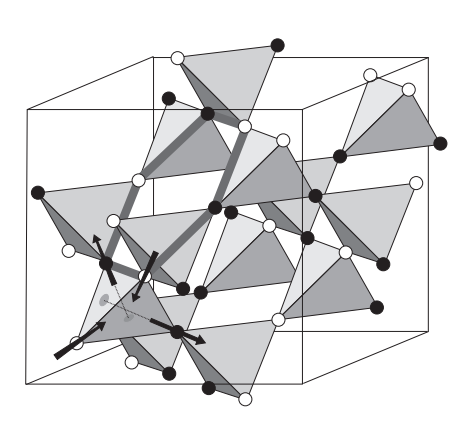
\includegraphics[width=1\linewidth]{New_figure/pyrochlor.png} \\ б)}
% 	\end{minipage}
% 	\caption{а) Расположение атомов водорода (черные кружки) вокруг атомов кислорода (белые кружки) во льду, б) Решетка пирохлора, состоящая из тетраэдров с общими углами, занятыми магнитными редкоземельными ионами в материалах спинового льда Ho$_2$Ti$_2$O$_7$ и Dy$_2$Ti$_2$O$_7$~\cite{bramwell2001}}
% 	\label{frustt}
% \end{figure}

\noindent момент, часто называемый как «спин», который в своем низкоэнергетическом состоянии должен удовлетворять принципу «два-входа---два-выхода» на каждом тетраэдре, образующем кристаллическую структуру~(рисунок~\ref{frustt}б). Первыми материалами, идентифицированными как спиновые льды, были пирохлоры Dy$_2$Ti$_2$O$_7$ (титанат диспрозия) и Ho$_2$Ti$_2$O$_7$ (титанат гольмия).

Сделаем важное отступление о том, что при отсутствии фрустрации при заданных параметрах обменных взаимодействий на двумерных решетках мы всегда получаем теплоемкость в виде острого $\Lambda$ - образного пика, при этом имеет место фазовый переход в критической точке~\cite{peierls1936}. А во фрустрированном состоянии всегда имеется пологий куполообразный пик и отсутствие фазового перехода, поскольку основное состояние системы оказывается сильно вырожденным. На рисунке \ref{tr} приведены графики теплоемкостей модели Изинга на треугольной решетке во фрустрированном и нефрустрированном состояниях.

Здесь и далее, термодинамические и магнитные величины, такие как свободная энергия $F$, энтропия $S$, теплоемкость $C$, намагниченность $M$ и другие, будут изображены на графиках через условные единицы, а именно постоянная Больцмана $k$ будет положена равной единице, а величины $T$ и $H$ будут измеряться в единицах $|J|$, как это принято в теории низкоразмерных систем.

% \begin{figure}[h]
% 	\begin{minipage}[h]{0.49\linewidth}
% 		\center{\includegraphics[width=1\linewidth]{New_figure/tr1.eps} \\ а)}
% 	\end{minipage}
% 	\hfill
% 	\begin{minipage}[h]{0.49\linewidth}
% 		\center{\includegraphics[width=1\linewidth]{New_figure/tr2.eps} \\ б)}
% 	\end{minipage}
% 	\caption{Теплоемкость модели Изинга на треугольной решетке: а) система фрустрирована ($J_1 = -1$, $J_2 = -1$, $J_3 = -1$), б) система не фрустрирована ($J_1 = -1$, $J_2 = -1$, $J_3 = 1$). Пунктирной линией обозначена температура фазового перехода}
% 	\label{tr}
% \end{figure}

Материалы спинового льда характеризуются случайным беспорядком в ориентации момента магнитных ионов, даже когда материал находится при очень низких температурах. Это находится в соответствии со случаем водяного льда. Об этом может свидетельствовать широкий гладкий пик теплоемкости, при котором, как уже известно, не возникает фазового перехода и наличие ненулевого значения нуль-температурной энтропии~(рисунок~\ref{frusttt}). 

% \begin{figure}[h]
% 	\begin{minipage}[h]{0.49\linewidth}
% 		\center{\includegraphics[width=1\linewidth]{New_figure/heat.png} \\ а)}
% 	\end{minipage}
% 	\hfill
% 	\begin{minipage}[h]{0.49\linewidth}
% 		\center{\includegraphics[width=1\linewidth]{New_figure/ent.png} \\ б)}
% 	\end{minipage}
% 	\caption{а) Теплоемкость и б) энтропия материала спинового льда Dy$_2$Ti$_2$O$_7$ в сравнении с результатами метода Монте-Карло, примененного для модели дипольного спинового льда~\cite{bramwell2001}}
% 	\label{frusttt}
% \end{figure}

Однако, среди многих типов магнитоупорядоченных веществ особое место принадлежит так называемым спиновым стеклам~\cite{diep2013,docenko1993}.  Обоснованием этого термина служит тот факт, что ориентация элементарных магнитных моментов атомов спинового стекла в области температур ниже некоторой величины $T_{\text{freeze}}$ не имеет никакой пространственной периодичности. В
отличие от парамагнетиков, где элементарные магнитные моменты флуктуируют во времени, спиновые стекла характеризуются наличием «замороженных» магнитных моментов~(рисунок~\ref{glass}).

% \begin{figure}[b]
% 	\center{\includegraphics[width=0.5\linewidth]{New_figure/glass.png}}
% 	\caption{Схематическое представление случайной спиновой структуры --- спинового стекла}
% 	\label{glass}
% \end{figure}

Типичные спиновые стекла представляют собой разбавленные магнитные сплавы Cu-Mn, Ag-Mn или Au-Fe, в которых магнитные моменты 3d-элементов взаимодействуют через дальнодействующее обменное взаимодействие. 

Для спиновых стекол характерно, что магнитный момент, наведенный в спиновом стекле внешним магнитным полем, зависит не только от величины поля, но также от предыстории образца. Кроме этого, отличительной чертой поведения спинового стекла является наличие резкого излома на температурной зависимости магнитной восприимчивости, измеренной при малых магнитных полях, а также линейная зависимость теплоемкости от температуры, что говорит о том, что основное состояние спинного стекла сильно вырожденно. 

Считается, что изучение спиновых стекол будет способствовать созданию более совершенных принципов компьютерной памяти. Зависимость магнитного состояния спинового стекла от его магнитной предыстории может использоваться для создания новых материалов магнитной памяти. Также, модель спинового стекла весьма полезна для понимания поведения определенных нейронных сетей, в особенности сетей Хопфилда (искусственная нейронная сеть, в которой каждый нейрон может принимать одно из двух состояний $\pm 1$)~\cite{aarts2001, kincel1987}. 

На одномерной изинговской решетке также наблюдаются фрустрации~\cite{zarubin2019}. Модель Изинга со спином $s = 1$ на одномерной решетке с учетом антиферромагнитного взаимодействия только между ближайшими соседями во внешнем магнитном поле является простейшей моделью, в которой можно обнаружить фрустрации. Ее наибольшее собственное значения уже было найдено в прошлом пункте и оно имеет вид:
\begin{equation}
\lambda_{\text{max}}= e^{\frac{J}{T}}\ch \bigg(\frac{H}{T}\bigg) + \sqrt{e^{\frac{2J}{T}}\ch^2 \bigg(\frac{H}{T}\bigg)-2\sh \bigg(\frac{2J}{T}\bigg)}.
\end{equation}

При $H=0, T=0$ система находится в основном состоянии, представляющее собой антиферромагнитное упорядочение ($\textdownarrow \textuparrow$, где $\textdownarrow$ --- спин направлен против магнитного поля, $\textuparrow$ - совпадает с направлением поля). С увеличением поля спины начнут выстраиваться вдоль магнитного поля, тем самым возникает ферромагнитная структура ($\textuparrow \textuparrow$). Можно показать, что в некотором поле, называемом фрустрирующим $H_{\text{fr}}$, энергии этих двух состояний совпадают, и имеется бесконечное количество различных конфигураций с одинаковой энергией. На рисунке \ref{nearestanti} показан этот механизм.

% \begin{figure}[h]
% 	\center{\includegraphics[width=0.65\linewidth]{New_figure/nearestanti.eps}}
% 	\caption{Конфигурации, возникающие в модели Изинга при учете ближайших соседей в магнитном поле, для каждой конфигурации приведена соответствующая энергия. Закрашенные кружочки --- спин направлен вверх, прозрачные --- вниз}
% 	\label{nearestanti}
% \end{figure}

Рассчитаем энергию антиферромагнитной структуры. Данное состояние следует назвать структурой с удвоением периода трансляций решетки, так как оно представляет собой последовательность повторяющихся сегментов $\textdownarrow \textuparrow$. Для определения энергии воспользуемся гамильтонианом \eqref{eq:1.2}, при этом достаточно посчитать энергию только для одного сегмента $\textdownarrow \textuparrow$:
\begin{equation}
E_{\textdownarrow \textuparrow}=-J s_{i}s_{i+1}-H s_{i} =\frac{1}{2}\left( \frac{J}{2}+\frac{J}{2}-H+\frac{J}{2}+\frac{J}{2}+H\right)=J.
\label{eq:2.2}
\end{equation}

Получилось, что энергия структуры, приходящаяся на один узел, находящейся в антиферромагнитном состоянии, представляется обменным взаимодействием между соседними узлами решетки.

Следуя тем же путем, можно определить энергию ферромагнитной структуры:
\begin{equation}
E_{\textuparrow \textuparrow} = -\frac{J}{2}-\frac{J}{2}-H= -J-H.
\label{eq:2.3}
\end{equation}

Приравнивая энергии \eqref{eq:2.2} и \eqref{eq:2.3} друг к другу, получаем величину фрустрирующего поля для случая взаимодействия только ближайших соседей:
\begin{equation}
H_{\text{fr}}=-2J.
\label{eq:2.4}
\end{equation}

К примеру, при $J=-1$ (антиферромагнитное упорядочивание), имеется фрустрирующее поле $H_{\text{fr}}=2$.

C помощью формул \eqref{eq:1.15} и \eqref{eq:1.17} можно показать, что в точке фрустрации при $T\rightarrow 0$ энтропия равна натуральному логарифму золотого сечения $S=\ln \left[\left(1+\sqrt{5}\right)\!/2\right]$, а намагниченность --- $M=1/\sqrt{5}$.

% \begin{figure}[h]
% 	\begin{minipage}[h]{0.49\linewidth}
% 		\center{\includegraphics[width=1\linewidth]{New_figure/mag1.eps} \\ а)}
% 	\end{minipage}
% 	\hfill
% 	\begin{minipage}[h]{0.49\linewidth}
% 		\center{\includegraphics[width=1\linewidth]{New_figure/mag2.eps} \\ б)}
% 	\end{minipage}
% 	\caption{а) Намагниченность как функция магнитного поля при $T\rightarrow 0$ и б) как функция температуры во фрустрирующем поле при $H_{\text{fr}}=2$ (сплошная линия), при $H_{\text{fr}}=1.95$ (синяя пунктирная линия) и при $H_{\text{fr}}=2.05$ (зеленая пунктирная линия)}
% 	\label{mag}
% \end{figure}

Итак, рассматривая систему при стремлении температуры к нулю, ее намагниченность испытывает скачок во фрустрирующем поле, таким образом, совершается переход между двумя определенными конфигурациями (рисунок \ref{mag}).

В точке фрустрации, с соответствующей нуль-температурной энтропией (рисунок \ref{fr}а), не равной нулю, помимо сходящихся фаз (структур с определенными трансляциями) наблюдается также и бесконечное множество конфигураций, в том числе и без какой-либо трансляционной инвариантности с одинаковой энергией и все вместе они сосуществуют. Однако, если отойти от фрустрации на малую величину магнитного поля (или обменного взаимодействия), то реализуется переход системы в одну какую-то конкретную фазу. Тем самым, система становится упорядоченной, а энтропия стремится к нулю.

% \begin{figure}[h]
% 	\begin{minipage}[h]{0.49\linewidth}
% 		\center{\includegraphics[width=1\linewidth]{New_figure/entfr.eps} \\ а)}
% 	\end{minipage}
% 	\hfill
% 	\begin{minipage}[h]{0.49\linewidth}
% 		\center{\includegraphics[width=1\linewidth]{New_figure/heatfr.eps} \\ б)}
% 	\end{minipage}
% 	\caption{а) Энтропия во фрустрирующем магнитном поле модели Изинга при учете взаимодействия между ближайшими соседями (сплошная линия). Красной пунктирной линией показана энтропия системы вблизи фрустрации и б) Расщепление теплоемкости около фрустрирующего поля в модели Изинга}
% 	\label{fr}
% \end{figure}

Теплоемкость же в непосредственной близости к фрустрации имеет два пика --- острый и широкий плавный~(рисунок~\ref{fr}б). Последний, к тому же, всегда находится правее (в стороне больших температур). Данный факт подтвержден экспериментально~\cite{matsumura1997} (около фрустрирующего поля происходит расщепление теплоемкости на два пика, см. рисунок~\ref{new1}). 

В заключение, стоит отметить любопытное предположение, выдвинутое нами в  статье~[A2] о качественном совпадении явления фрустрации с явлением критической опалесценции. Так как в местах схождения сразу нескольких фаз, фазы не индивидуализированы, а существенно фрустрированы так как, кроме сходящихся фаз, в точках фрустраций существует бесконечное множество конфигураций без каких-либо трансляционных инвариантностей, чему свидетельствует ненулевая нуль-температурная энтропия. А в работе Смолуховского~\cite{smoluchowski1907} установлено, что явление критической опалесценции обусловлено возникновением в тройной точке бесконечного множества термодинамических флуктуаций, поэтому фактически можно сказать, что в тройной точке возникает явление сильных фрустраций.

% \begin{figure}[H]
% 	\center{\includegraphics[width=1\linewidth]{New_figure/new1.eps}}
% 	\caption{Магнитная теплоемкость TmTe для двух направлений внешнего поля а) [100] и б) [111]~\cite{matsumura1997}}
% 	\label{new1}
% \end{figure}

\section{Комбинаторный метод Вдовиченко--Фейнмана}\label{sec:markup}

Идея комбинаторного решения модели Изинга на двумерной решетке принадлежит Фейнману. Суть метода заключается в подсчете всех суперпозиций замкнутых многоугольников (не имеющих общих сторон) на двумерной решетке. Впоследствие, предположение Фейнмана развивалось в статьях Каца и Уорда~\cite{kac1952}, Монтролла~\cite{montroll1953} и Вдовиченко~\cite{vdovichenko1965}. Так или иначе, метод берет свое начало с высокотемпературного разложения статистической суммы двумерной решетки. 

Рассмотрим квадратную решетку с $M$ горизонтальными связями и с $M$ вертикальными связями. В термодинамическом пределе $M \rightarrow \infty$ и $M$ совпадает с количеством узлов в решетке $N$. 

Далее, рассмотрим гамильтониан с разными обменными взаимодействиями: по горизонтальному направлению --- $J$, а по вертикальному направлению --- $J^{'}$.

Тогда для статистической суммы модели при нулевом магнитном поле имеем
\begin{equation}
Z_{N} = \sum_{\{\sigma\}} \exp{\bigg[ K_1 \sum_{(i,j)} \sigma_i \sigma_j + K_2 \sum_{(i,k)} \sigma_i \sigma_k\bigg]},
\end{equation}
где первая сумма идет по спинам в горизонтальном направлении, а вторая сумма по спинам в вертикальном направлении
\begin{equation*}
K_1 = \frac{J}{T}; \;\;\;\;\;\; K_2 = \frac{J^{'}}{T}.
\end{equation*}

Используя тождество
\begin{equation}
\exp{[x\sigma_i \sigma_l]} = \ch x (1 + \sigma_i \sigma_l \th x),
\end{equation}
статистическая сумма может быть переписана в виде
\begin{equation}
Z_{N} = (\ch K_1 \ch K_2)^M \sum_{\{\sigma\}} \prod_{(i,j)} (1 + v \sigma_i \sigma_j) \prod_{(i,k)} (1 + w \sigma_i \sigma_k),
\label{zn1} 
\end{equation}
\begin{equation*}
v = \th K_1; \;\;\;\;\;\; w = \th K_2.
\end{equation*}

Оба параметра $v$ и $w$ всегда меньше 1 для всех значений температуры $T$, кроме $T = 0$, при котором $v = w = 1$. В частности, они являются малыми параметрами в высокотемпературном разложении, поэтому следует искать разложение статсуммы вблизи $T = \infty$.

Если разложить произведение в формуле \eqref{zn1}, получится $2^{2M}$ слагаемых, поскольку имеется $2M$ множителей (по одному на каждый сегмент)
и в каждом из них есть два слагаемых. Можно ввести графическое представление этого разложения. Линия, проведенная между узлами решетки по горизонтали $(i, j)$, соответствует множителю $v \sigma_i \sigma_j$, линия, проведенная между узлами решетки по вертикали  $(i, k)$, соответствует множителю $v \sigma_i \sigma_k$. Отсутствие линии между узлами решетки соответствует множителю 1. Повторяя данную операцию для $2^{2M}$ слагаемых, можно установить соответствие между членами в разложении и графическими конфигурациями. Общее выражении этих слагаемых таково
\begin{equation*}
v^r w^s \sigma_1^{n_1} \sigma_2^{n_2} \sigma_3^{n_3} \dots.
\end{equation*}
где $r$ --- общее число горизонтальных связей, $s$ --- общее число вертикальных связей, $n_i$ --- количество линий, где $i$ --- конечный узел. 

Теперь необходимо посчитать сумму по всем спинам решетки, чтобы получить статсумму. Поскольку каждый спин $\sigma_i$ принимает значения $\pm 1$, получаем нулевую сумму, если все $n_1$, $n_2$, \dots, $n_N$ являются четными и этом случае результат равен $2^N v^r w^s$. Исходя из этих соображений, статистическая сумма может быть выражена как

\begin{equation}
Z_{N} = 2^N (\ch K_1 \ch K_2)^M \sum_{P} v^{r} w^{s}, 
\end{equation}
где сумма идет по всем конфигурациям линий на решетке с четным количеством линий на каждом узле решетки, то есть сумма взята по всем замкнутым многоугольникам $P$ решетки. Таким образом, статсумма, не считая множителя, задается геометрической величиной
\begin{equation}
\Phi(v, w) = \sum_{P} v^r w^s.
\label{phi}
\end{equation}

Вычислить первые члены этой суммы нетрудно. Первый член равен 1 и
соответствует случаю, когда на решетке нет многоугольников. Второй член
соответствует наименьшему замкнутому многоугольнику на решетке, т.е. квадрату с единичной длиной, как показано на рисунке \ref{figf}. Количество таких квадратов равно $N$, так как они могут размещаться на любом из $N$ узлов решетки. Каждый из них имеет вес $(vw)^2$, поэтому второй член суммы \eqref{phi} равен $N(vw)^2$. Следующая замкнутая фигура представляет собой прямоугольник из 6 связей, их может быть два вида: $v^4 w^2$ и $v^2 w^4$, как показано на рисунке \ref{figff}. Количество таких прямоугольников также может быть $N$ штук. Используя эти первые члены разложения функции $\Phi(v, w)$ запишем
\begin{equation}
\Phi(v, w) = 1 + N (vw)^2 + N (v^4 w^2 + v^2 w^4) + \dots.
\end{equation}

% \begin{figure}[h]
% 	\center{\includegraphics[width=0.4\linewidth]{New_figure/f.eps}}
% 	\caption{Второй член высокотемпературного разложения}
% 	\label{figf}
% \end{figure} 

% \begin{figure}[h]
% 	\center{\includegraphics[width=0.4\linewidth]{New_figure/ff.eps}}
% 	\caption{Третий член высокотемпературного разложения}
% 	\label{figff}
% \end{figure} 

Следовательно, для знания статсуммы нужно посчитать все члены в разложении $\Phi(v, w)$, однако вычисление следующих членов $\Phi(v, w)$ стремительно усложняется. 

Изящное решение данной проблемы было предложено Вдовиченко~\cite{vdovichenko1965}. Метод решения подразделяется на три шага: (a) первый шаг состоит в выражении суммы по многоугольникам в виде суммы по замкнутым циклам без пересечений; (б) второй шаг заключается в преобразовании суммы по замкнутым циклам без пересечений в сумму по всем возможным замкнутым циклам; (в) на последнем шаге задача сводится к случайному блужданию по решетке.

% \begin{figure}[h]
% 	\center{\includegraphics[width=0.4\linewidth]{New_figure/pict.eps}}
% 	\caption{Непересекающиеся многоугольники}
% 	\label{figpict}
% \end{figure}   

% \begin{figure}[h]
% 	\center{\includegraphics[width=0.4\linewidth]{New_figure/pic.eps}}
% 	\caption{Самопересекающийся многоугольник}
% 	\label{figpic}
% \end{figure}  

Обсудим реализацию первого шага, то есть как организовать сумму по многоугольникам с точки зрения их соединенных частей. Заметим, что каждый многоугольник состоит из одной или нескольких связанных частей. Для несамопересекающихся многоугольников это утверждение очевидно: например, многоугольник на рисунке \ref{figpict} состоит из двух несвязных частей. Но для самопересекающихся многоугольников утверждение может быть неоднозначным, и в зависимости от разложения могут быть разные связанные части. Чтобы прояснить этот вопрос, рассмотрим многоугольник на рисунке \ref{figpic}. Его можно разложить тремя разными способами, как показано на рисунке \ref{figvar}: его можно разложить на одну или две соединенные части без пересечения или в одну соединенную часть, но с пересечением. Легко показать, что это правило является общим, а именно всегда существует три возможных разложения для всех самопересечений многоугольников. 

% \begin{figure}[b]
% 	\center{\includegraphics[width=0.5\linewidth]{New_figure/var.eps}}
% 	\caption{Три различных разложения на связные части для самопересекающегося многоугольника}
% 	\label{figvar}
% \end{figure}

% \begin{figure}[h]
% 	\center{\includegraphics[width=0.5\linewidth]{New_figure/graph.eps}}
% 	\caption{Многоугольник с повторяющимися связями}
% 	\label{figgraph}
% \end{figure}

Сумма по многоугольникам, указанная в уравнении \eqref{phi}, может быть организована в сумму по соединенным частям многоугольников, но нужно действовать осторожно, чтобы правильно подсчитать различные члены разложения, в частности, чтобы не подсчитывать одну и ту же конфигурацию более одного раза. Эта проблема может быть решена путем взвешивания каждого многоугольника с коэффициентом $(-1)^n$, где $n$ - общее количество самопересечений замкнутого многоугольника. Таким образом, все лишние члены в сумме исчезают. В примере на рисунке \ref{figvar} первые два члена имеют вес $+1$, а последний член $-1$, так что в окончательном выражении сохраняется только один член.

Обратите внимание, что, приняв приведенный выше рецепт для выполнения суммирования по замкнутым многоугольникам, можно включить в сумму также многоугольники с повторяющимися связями. Простейший из них представлен на рисунке \ref{figgraph}. Эти многоугольники явно отсутствуют в исходной формулировке высокотемпературного разложения, так как на некоторых узлах имеется нечетное количество связей. Однако, учитывая вес связи, легко увидеть, что эти члены в сумме сокращаются.

Однако, по-прежнему существует недостаток в процедуре взвешивания многоугольника, поскольку он зависит от глобального свойства многоугольника, такого как количество его пересечений. Было бы удобнее выразить вес $(−1)^n$ локальным способом. Это возможно благодаря известному геометрическому свойству: общий угол поворота касательной, проходящей вокруг замкнутого плоского контура, равен $2\pi (\xi + 1)$, где $\xi$ - целое число (положительное или отрицательное), с четностью, совпадающей с номером $\nu$ самопересечения замкнутого многоугольника. Следовательно, мы можем присвоить каждой точке замкнутого многоугольника фазовый множитель $e^{i\alpha / 2}$, где угол поворота $\alpha$ принимает значения $\alpha = 0, \pm \pi/ 2$ в соответствии с углом изменения направления на следующую связь, так что произведение всех этих множителей по петле дает $(−1)^{\nu + 1}$. Для набора из $k$ петель имеем $(−1)^{n + k}$, где $n = \sum \nu$.

Таким образом, мы можем автоматически учитывать количество самопересечений многоугольника, взвешивая каждый узел на $e^{i\alpha/2}$ и умножая член, соответствующий данному многоугольнику (заданному набором из $k$ петель), на множитель $(−1)^k$, поскольку этот член будет компенсировать то же слагаемое, что и в предыдущем выражении $(-1)^{n + k}$.

Далее для простоты повествования рассмотрим только изотропный случай квадратной решетки, а именно, когда обменное взаимодействие в горизонтальном и вертикальном направлениях одинаково, так что в статистическую сумму входит только параметр $v = \th K$, где $K = J/T$. Тогда статсумма такой решетки будет даваться выражением
\begin{equation}
Z_N = 2^N \ch^{2N} \!\!K\; \Phi(v),
\label{zn2}
\end{equation}
при
\[ \Phi(v) = \sum_r g_r v^r, \]
где $g_r$ --- количество замкнутых необязательно связанных многоугольников, заданных четным числом $r$ связей.

Обозначим через $f_{r}$ сумму по отдельным замкнутым многоугольникам, состоящих из $r$ звеньев. Каждый многоугольник взвешен в соответствии с указанным выше правилом. Сумма по всем парам многоугольников с общим числом звеньев $r$ определяется выражением
\begin{equation*}
\frac{1}{2!} \sum_{\substack{r_1 + r_2 = r}} f_{r_1} f_{r_2},
\end{equation*}
где множитель $2!$ в знаменателе учитывает, что перестановка двух индексов приводит к одной и той же паре замкнутых многоугольникам. Аналогичный множитель $n!$ присутствует в знаменателе суммы для $n$ многоугольников.

Следовательно, функцию $\Phi$ можно записать как
\begin{equation}
\Phi(v) = \sum_{n = 0} (-1)^n \frac{1}{n!} \sum_{\substack{r_1, r_2, \dots = 1}} v^{r_1 + r_2 + \dots + r_n} f_{r_1} \dots f_{r_n}.
\end{equation}

Поскольку в $\Phi$ есть члены, соответствующие множествам петель с любой возможной общей длиной $r = r_1 + r_2 + \dots$, в сумме  индексы $r_1, r_2, \dots$ принимают независимо все значения от $1$ до $\infty$, так что
\begin{equation*}
\sum_{\substack{r_1, r_2, \dots}} v^{r_1 + r_2 + \dots + r_n} f_{r_1} \dots f_{r_n} = \bigg(\sum_{r=1}^{\infty}v^r f_{r}\bigg)^n.
\end{equation*}

Таким образом, $\Phi$ выражается как
\begin{equation}
\Phi (v) = \exp{\bigg[-\sum_{r=1}^{\infty}v^r f_{r}\bigg]}.
\label{Phi}
\end{equation}

Этим выражением завершаются шаги (а) и (б) метода Вдовиченко.
Остается только явно вычислить величину $f_{r}$.

% \begin{figure}[h]
% 	\center{\includegraphics[width=0.5\linewidth]{New_figure/dir.eps}}
% 	\caption{Возможные направления движения по квадратной решетке}
% 	\label{figdir}
% \end{figure}

Поскольку на квадратной решетке есть четыре различных направления, по которым можно передвигаться, то их удобно пронумеровать индексом $\mu = 1, 2, 3, 4$, как показано на рисунке \ref{figdir}. Введем новую функцию $W_r (i, j, \mu)$, которая определяется как сумма по всем возможным путям длины $r$, начинающиеся из заданной точки с координатами $(i_0, j_0)$ вдоль направления $\mu_0$ и достигая в точке координаты $(i, j)$ вдоль направления $\mu$. Пути, входящие в определение $W_r (i, j, \mu)$, взвешиваются с учетом ранее введенных множителей $e^{i\alpha / 2}$. Если теперь выбрать $(i_0, j_0)$ в качестве начальной точки, $W_r (i_0, j_0, \mu_0)$ станет суммой по всем многоугольникам, выходящим и возвращающимся в ту же точку. В результате, имеем тождество
\begin{equation}
f_{r} = \frac{1}{2r} \sum_{i_0, j_0, \mu} W_r (i_0, j_0, \mu),
\label{fl}
\end{equation}
где член $1 / (2r)$ учитывает тот факт, что в сумме в правой части каждый замкнутый многоугольник может быть пересечен в двух противоположных направлениях и может иметь любой из своих $r$ узлов в качестве отправной точки. Благодаря своему определению, функция $W_r (i, j, \mu)$ удовлетворяет рекурсивным уравнениям
\begin{align}
&W_{r+1} (i, j, 1) = W_r (i − 1, j, 1) + e^{−i \frac{\pi}{4}} W_r (i, j − 1, 2) + 0 + e^{i \frac{\pi}{4}} W_r (i, j + 1, 4), \nonumber \\
&W_{r+1} (i, j, 2) = e^{i \frac{\pi}{4}} W_r (i − 1, j, 1) + W_r (i, j − 1, 2) + e^{−i \frac{\pi}{4}} W_r (i + 1, j, 3) + 0, \nonumber\\
& W_{r+1} (i, j, 3) = 0 + e^{−i \frac{\pi}{4}} W_r (i, j − 1, 2) + W_r (i + 1, j, 3) + e^{-i\frac{\pi}{4}} W_r (i, j + 1, 4), \nonumber\\
& W_{r+1} (i, j, 4) = e^{−i \frac{\pi}{4}} W_r (i − 1, j, 1) + 0 + e^{i \frac{\pi}{4}} W_r (i + 1, j, 3) + W_r (i, j + 1, 4).
\label{eq}
\end{align}

Рассмотрим, например, первое уравнение \eqref{eq}. В точку $i$, $j$, $1$ можно попасть, сделав последний $(r + 1)$-й шаг слева, снизу или сверху, но не справа. Коэффициенты, представленные в уравнении, основаны на фазовых факторах, относящихся к изменению направлений. Используя те же аргументы, можно вывести другие уравнения в \eqref{eq}. Вводя матрицу коэффициентов $\Lambda$, рекурсивные уравнения можно записать в виде
\begin{equation}
W_{r+1}(i, j, \mu) = \sum_{i^{'},\; j^{'},\; \mu^{'}} \Lambda (ij\mu\; |\; i^{'}j^{'}\mu^{'}) W_{r} (i^{'}, j^{'}, \mu^{'}),
\end{equation}
которые допускают наводящую на размышления интерпретацию: эти уравнения можно интерпретировать как марковский процесс, связанный со случайным блужданием по решетке, с вероятностью перехода между двумя ближайшими соседними узлами, выраженными относительным матричным элементом $\Lambda$. Поскольку существует четыре возможных направления для этого движения, при сохранении всех остальных параметров фиксированными, $\Lambda$ представляет собой матрицу $4 \times 4$ с индексами $\mu^{'}$ и $\mu$, графическая интерпретация которой показана на рисунке \ref{figmatx}.

% \begin{figure}[h]
% 	\center{\includegraphics[width=0.5\linewidth]{New_figure/matx.eps}}
% 	\caption{Элементы матрицы $\Lambda$}
% 	\label{figmatx}
% \end{figure}

В свете приведенной выше интерпретации рекурсивных уравнений вероятность перехода относительно пути полной длины $r$ выражается матрицей $\Lambda^r$. Обратите внимание, что диагональные элементы этой матрицы выражают вероятность вернуться в исходную точку после прохождения цикла длины $r$, т.е. они совпадают с $W_r (i_0, j_0, \mu_0)$. Следовательно, имеем 
\begin{equation}
\Sp \Lambda^r = \sum_{i_0, j_0, \mu} W_r (i_0, j_0, \mu),
\end{equation}
и, сравнивая с \eqref{fl}, приходим к
\begin{equation}
f_r = \frac{1}{2r} \Sp \Lambda^r = \frac{1}{2r} \sum_a \lambda_a^r,
\end{equation}
где $\lambda_a$ - собственные значения матрицы $\Lambda$. Используя это выражение в \eqref{Phi} и меняя местами индексы суммы, получаем
\begin{multline}
\Phi(v) = \exp{\bigg[-\frac{1}{2}\sum_i \sum_{r=1}\frac{1}{r} v^r \lambda_i^r\bigg]} = \\ = \exp{\bigg[\frac{1}{2}\sum_i \ln(1 -  v\lambda_i)\bigg]} = \prod_i \sqrt{1 - v\lambda_i}.
\end{multline}

Последнее, что нужно сделать --- это определить собственные значения $\Lambda$. Диагонализация этой матрицы по координатам $k$ и $l$ решетки может быть легко выполнена с помощью преобразования Фурье. Фактически, определяя
\begin{equation}
W_r (p, q, \mu) = \sum_{k,l = 0} e^{-\frac{2\pi i}{L}(pk + ql)} W_r (k, l, \mu),
\end{equation}
с $N = L^2$ и преобразованием Фурье  имеем
\begin{align*}
&W_{r+1} (p, q, 1) = \epsilon^{-p}\; W_r (p, q, 1) + \epsilon^{-q} \alpha^{-1}\;  W_r (p, q, 2) + \epsilon^{q} \alpha\; W_r (p, q, 4),\\
&W_{r+1} (p, q, 2) = \epsilon^{-p} \alpha\; W_r (p, q, 1) + \epsilon^{-q}\; W_r (p, q, 2) + \epsilon^{p} \alpha^{-1}\; W_r (p, q, 3),\\
& W_{r+1} (p, q, 3) = \epsilon^{-q} \alpha\; W_r (p, q, 2) + \epsilon^{p}\; W_r (p, q, 3) + \epsilon^{q} \alpha^{-1}\; W_r (p, q, 4),\\
& W_{r+1} (p, q, 4) = \epsilon^{-p} \alpha^{-1}\; W_r (p, q, 1) + \epsilon^{p} \alpha\; W_r (p, q, 3) + \epsilon^{q}\; W_r (p, q, 4),
\end{align*}
где $\epsilon = e^{2\pi i/L}$ и $\alpha = e^{i\pi/4}$.

Поскольку $W_r (p, q, \mu)$ появляется с одинаковыми индексами $p$ и $q$ как в левой, так и в правой частях этих уравнений, преобразование Фурье матрицы $\Lambda$ диагонально по этим индексам, и мы имеем
\begin{equation}
\Lambda (p, q, \mu\; |\; p, q, \mu^{'}) = 
\begin{pmatrix}
\epsilon^{-p} & \alpha^{-1}\epsilon^{-q} & 0 & \alpha \epsilon^{q}  \\
\alpha \epsilon^{-p} & \epsilon^{-q} & \alpha^{-1}\epsilon^{p} & 0 \\
0 & \alpha\epsilon^{-q} & \epsilon^{p} & \alpha^{-1} \epsilon^{q}  \\
\alpha^{-1} \epsilon^{-p} & 0 & \alpha \epsilon^{p} & \epsilon^{q}  \\
\end{pmatrix}.
\end{equation}

Несложное вычисление показывает, что
\begin{multline}
\prod_i (1 - v\lambda_i) = \Det(I - \Lambda) = \\ = (1 + v^2)^2 - 2v (1 - v^2) \bigg(\!\!\cos \frac{2 \pi p}{L} + \cos \frac{2 \pi q}{L}\bigg),
\end{multline}
где $I$ --- единичная матрица размером $4 \times 4$.

Возвращаясь к выражению \eqref{zn2}, имеем
\begin{equation}
Z_{N} = 2^N (\ch K)^{2N} \prod_{p, q}^{L} \bigg[ (1 + v^2)^2 - 2v (1 - v^2) \bigg(\!\!\cos \frac{2 \pi p}{L} + \cos \frac{2 \pi q}{L}\bigg) \bigg]^{1/2}.
\end{equation}

Прологарифмировав обе части уравнения, получаем
\begin{multline}
\ln Z_N = N\ln 2 + 2N\ln (\ch K) + \frac{1}{2} \sum_{p,q = 0}^{L} \ln \bigg[ (1 + v^2)^2 - \\ - 2v (1 - v^2) \bigg(\!\!\cos \frac{2 \pi p}{L} + \cos \frac{2 \pi q}{L}\bigg) \bigg]. 
\end{multline}

Введем обозначения $\omega_1 = 2 \pi p / L$ и $\omega_2 = 2 \pi q /L$, также, при $L \rightarrow \infty$ сумма становится интегралом 
\begin{multline}
\ln \frac{\lambda_s}{2} = 2\ln (\ch K) + \frac{1}{8 \pi^2} \int_{0}^{2\pi} \int_{0}^{2\pi} \ln \big[ (1 + v^2)^2 - \\ - 2v (1 - v^2) (\cos \omega_1 + \cos \omega_2) \big] d \omega_1 d \omega_2.
\end{multline}

Учитывая, что $v = \th K$, после всех упрощений окончательно получаем выражение для статистической суммы (приходящейся на один узел) изотропной ($K_1 = K_2 = K $) квадратной решетки
\begin{equation}
\ln \frac{\lambda_s}{2} = \frac{1}{8 \pi^2} \int_{0}^{2\pi} \int_{0}^{2\pi} \ln \big[ \ch^2 2K - \sh 2K( \cos \omega_1 + \cos \omega_2)\big] d \omega_1 d \omega_2,
\end{equation} 
где $K = J/T$. 

Можно показать, что матрица коэффициентов $\Lambda$ для неизотропной решетки ($K_1 \neq K_2$) статсуммы \eqref{zn1} записывается в следующем виде
\begin{equation}
\Lambda (p, q, \mu\; |\; p, q, \mu^{'}) = 
\begin{pmatrix}
v\epsilon^{-p} & w\alpha^{-1}\epsilon^{-q} & 0 & w\alpha \epsilon^{q}  \\
v\alpha \epsilon^{-p} & w\epsilon^{-q} & v\alpha^{-1}\epsilon^{p} & 0 \\
0 & w\alpha\epsilon^{-q} & v\epsilon^{p} & w\alpha^{-1} \epsilon^{q}  \\
v\alpha^{-1} \epsilon^{-p} & 0 & v\alpha \epsilon^{p} & w\epsilon^{q}  \\
\end{pmatrix}.
\end{equation}

Вычисляя определитель этой матрицы, получаем 
\begin{multline}
\prod_i (1 - \lambda_i) = \Det(I - \Lambda) = (1 + v^2)(1 + w^2) -\\- 2w (1 - v^2) \cos \frac{2 \pi p}{L}-  2v (1 - w^2) \cos \frac{2 \pi q}{L}.
\end{multline}

Тогда статсумма \eqref{zn1} может быть записана в форме
\begin{multline}
Z_{N} = 2^N (\ch K_1 \ch K_2 )^N \prod_{p, q}^{L} \bigg[ (1 + v^2)(1 + w^2) -\\- 2w (1 - v^2) \cos \frac{2 \pi p}{L}- 2v (1 - w^2) \cos \frac{2 \pi q}{L} \bigg]^{1/2}.
\end{multline}

При $v = \th K_1$ и $w = \th K_2$ приходим к окончательному выражению для статистической суммы (приходящейся на один узел) обычной квадратной решетки
\begin{equation}
\ln \frac{\lambda_s}{2} = \frac{1}{8 \pi^2} \int_{0}^{2\pi} \int_{0}^{2\pi} \ln \big[ \ch 2K_1 \ch 2K_2 - \sh 2K_1 \cos \omega_1 - \sh 2K_2 \cos \omega_2\big] d \omega_1 d \omega_2,
\end{equation} 
($K_1 = J/T$, $K_2 = J^{'}/T)$.


\section{Температура фазового перехода}

Точка перехода по своей сути является температурой, при которой реализуется переход системы из ферромагнитного (или антиферромагнитного) состояния в парамагнитную конфигурацию. При этом теплоемкость системы, как мы видели, испытывает кардинальное изменение, такое что в точке фазового перехода теплоемкость устремляется в бесконечность. Такой переход называется фазовым переходом второго рода.

Для нахождения точки перехода у определенной двумерной решетки достаточно лишь рассмотреть подынтегральное выражение точного решения. Подынтегральное выражение, являясь натуральным логарифмом, имеет одну особую точку в нуле, в которой интеграл расходится. Поэтому, чтобы найти температуру перехода $T_c$, приравнивают подлогарифмическое выражение нулю, после чего выражают температуру $T_c$:
\begin{equation*}
\int_{0}^{2\pi}\int_{0}^{2\pi} \ln \xi(J, T_c, \omega_1, \omega_2) d\omega_1 d\omega_2\;\;  \rightarrow\;\; \xi(J, T_c, \omega_1, \omega_2) = 0\;\; \rightarrow\;\; T_c.
\end{equation*}

К примеру, рассмотрим обычную квадратную решетку. Подлогарифмичекое выражение приравниваем нулю
\begin{equation}
\ch \bigg(\frac{2J_1}{T_c}\bigg) \ch \bigg(\frac{2J_2}{T_c}\bigg) - \sh \bigg(\frac{2J_1}{T_c}\bigg) \cos \omega_1 - \sh \bigg(\frac{2J_2}{T_c}\bigg) \cos \omega_2 = 0.
\end{equation}

% \begin{figure}[h]
% 	\center{\includegraphics[width=0.6\linewidth]{New_figure/tc.eps}}
% 	\caption{Выбор $\omega_1$ и $\omega_2$}
% 	\label{tc}
% \end{figure}

На данном этапе надо определиться при каких углах $\omega_1$ и $\omega_2$ следует искать критическую температуру $T_c$. Обычно $(\omega_1, \omega_2)$  принимают равными $(0, 0)$, $(0, \pi)$, $(\pi, 0)$ или $(\pi, \pi)$ соответственно. Другие углы, отличные от приведенных, дают аналогичные результаты из-за свойства трансляционной инвариантности (рисунок \ref{tc}). Кроме того, обменные взаимодействия $J_1$ и $J_2$ могут быть различными, а именно возможны четыре варианта: антиферромагнитное-антиферромагнитное, антиферромагнитное-ферромагнитное, ферромагнитное-антиферромагнитное, ферромагнитное-ферромагнитное.

% \begin{figure}[h]
% 	\center{\includegraphics[width=0.6\linewidth]{New_figure/tc2.eps}}
% 	\caption{Температурные зависимости подынтегральных выражений точного решения обычной квадратной решетки ($|J_1| = |J_2| = 1$). Синей кривой соответствуют случаи: 1) $\omega_1 = 0, \omega_2 = 0$, $J_1 > 0$, $J_2 > 0$, 2) $\omega_1 = 0$, $\omega_2 = \pi$, $J_1 > 0$, $J_2 < 0$, 3) $\omega_1 = \pi$, $\omega_2 = 0$, $J_1 < 0$, $J_2 > 0$, 4) $\omega_1 = \pi$, $\omega_2 = \pi$, $J_1 < 0$, $J_2 < 0$. Красная кривая соответствует отсутствию фазового перехода}
% 	\label{tcc}
% \end{figure}

Расхождения подлогарифмического выражения и, как следствие, получение температуры перехода~(рисунок~\ref{tcc}, для конкретики мы выбрали $|J_1| = |J_2| = 1$) можно добиться, рассматривая выражение~\eqref{tc}, например, в следующих случаях:
\begin{enumerate}
    \item $\omega_1 = 0, \omega_2 = 0, J_1 > 0, J_2 > 0$.
    \item $\omega_1 = 0, \omega_2 = \pi, J_1 > 0, J_2 < 0$.
    \item $\omega_1 = \pi, \omega_2 = 0, J_1 < 0, J_2 > 0$.
    \item $\omega_1 = \pi, \omega_2 = \pi, J_1 < 0, J_2 < 0$.
\end{enumerate}

В том или ином случае, температура перехода на обычной квадратной решетке выражается в виде
\begin{align}
T_c^{square} &= \frac{2J}{\ln [1 + \sqrt{2}]};& T_c^{square} &= J\cdot 2.2692\dots.
\end{align}

\section{Понятие декорированной решетки} 

В современной физике конденсированного состояния активно исследуются модели магнитных материалов, в которых кроме обменных взаимодействий учитываются разные усложняющие факторы, не учитываемые моделями первого приближения. Данные факторы позволяют оказывать значительное влияние на характер критического поведения магнетиков и приводить к существованию большого разнообразия магнитных упорядоченных состояний и фазовых переходов между ними. За последнее время значительно возрос интерес к исследованию декорированных структур.

Термин \guillemotleft декорированная решетка\guillemotright \hspace{1pt} был введен в работе Сиози~\cite{siozi1951}, после чего данная концепция начала стремительно развиваться другими авторами~\cite{siozi_domb1972, fisher1958}. Изучение данной области уже довольно богато литературой (см., например,~\cite{jaščur2016}--\cite{mutalamov2020}). Это можно объяснить тем, что декорирование порождает ряд новых, еще не до конца изученных эффектов по сравнению с исходными недекорированными решетками. В частности, декорирование порождает многообразие различных фрустрационных эффектов, может приводить как к подавлению фазовых переходов, присущих недекорированным решеткам, так и к возникновению новых фазовых переходов. Вместе с тем, появляются новые типы частичного упорядочения, а также различные формы расщепления теплоемкости. Богатство критического поведения декорированных решеток обусловлено возможностью многократного декорирования.

Суть построения декорированной решетки заключается во введении дополнительных спинов в промежутки между узлами исходной решетки~\cite{siozi_domb1972}. Данную процедуру можно реализовывать и в обратном порядке, превращая декорированные решетки в обычные. Основные спины еще называют нодальными, а дополнительные спины --- декорационными (рисунок \ref{decorsq}). Практически большинство реальных структур является декорированными.

% \begin{figure}[t]
% 	\center{\includegraphics[width=0.6\linewidth]{New_figure/decorsq.eps}}
% 	\caption{Декорированная квадратная решетка (единожды декорирована в горизонтальном направлении и дважды декорирована в вертикальном направлении). Синим цветом обозначены нодальные спины, красным --- декорационные спины}
% 	\label{decorsq}
% \end{figure}

% \begin{figure}[h]
% 	\center{\includegraphics[width=1\linewidth]{New_figure/cycle.png}}
% 	\caption{Циклическое преобразование решеток: $d$ --- дуальное преобразование, $Y - \Delta$ --- преобразование \guillemotleft звезда-треугольник\guillemotright \hspace{1pt}, $I$ --- декорационное преобразование~\cite{siozi_domb1972}}
% 	\label{cycle}
% \end{figure}

Стоит отметить, что точного аналитического решения модели Изинга на декорированной решетке в магнитном поле до настоящего момента получено не было~\cite{kassan-ogly2019}--\cite{kassan-ogly2020}. И только в настоящей работе мы приводим впервые полученное точное решение модели Изинга на декорированной решетке при наличии магнитного поля~[A3].

Напоследок, следует обратить внимание, что, наряду с дуальным преобразованием (преобразование обычной решетки в решетку к ней дуальную, которое идет посредством помещения в центр ячейки исходной решетки узла, после чего эти узлы соединяются, образуя дуальную решетку) и преобразованием \guillemotleft звезда-треугольник\guillemotright \hspace{1pt}, декорационное преобразование является важной процедурой при переходе от одной решетки к решетке совершенно иной топологии (рисунок \ref{cycle}).

\section{Постановка задачи исследования}

Цель настоящей магистерской диссертации заключается в рассмотрении обобщенной модели Изинга с произвольным количеством различных обменных взаимодействий как между ближайшими, так и между вторыми соседями с учетом декорирования и магнитного поля на одномерной цепочке, а также обобщенной модели Изинга с четырьмя различными обменными взаимодействиями между ближайшими соседями на квадратной решетке, с последующим изучением их термодинамических, магнитных и фрустрационных свойств.

Для достижения цели были поставлены следующие задачи:
\begin{enumerate}
    \item Получить точное аналитическое решение обобщенной модели Изинга на одномерной цепочке при учете магнитного поля методом трансфер-матрицы Крамерса-Ваннье.
    \item Исследовать термодинамические, магнитные и фрустрационные свойства обобщенной модели Изинга на одномерной цепочке, в том числе при учете декорирования.
    \item Получить точное аналитическое решение обобщенной модели Изинга на квадратной решетке комбинаторным методом Вдовиченко--Фейнмана.
    \item Исследовать термодинамические и фрустрационные свойства обобщенной модели Изинга на квадратной решетке.
\end{enumerate}

\FloatBarrier
           % Глава 1
\chapter{Обобщенная модель Изинга на одномерной цепочке при учете магнитного поля}\label{ch:ch2}

Начнем исследование модели Изинга с одномерного случая, поскольку он не представляет существенных вычислительных трудностей и в данном рассмотрении имеется возможность получения точных аналитических решений модели Изинга в присутствии магнитного поля.

\section{Обобщение модели Изинга на произвольное число трансляций линейной цепочки}\label{sec:ch2/sec1}

Гамильтониан обобщенной модели Изинга с произвольным числом обменных взаимодействий между ближайшими и вторыми соседями~\cite{kassan-ogly2001, dobson1969} линейной цепочки, находящейся в магнитном поле, может быть записан в следующей форме
\begin{multline}
\mathcal{H}_n(s)=-J_1\sum_{i=1,n+1,2n+1,\dots}^{N-n+1} s_i s_{i+1} - J_1^{'}\sum_{i=1,n+1,2n+1,\dots}^{N-n+1} s_i s_{i+2} -\\-J_2\sum_{i=2,n+2,2n+2,\dots}^{N-n+2} s_{i+1} s_{i+2} -J_2^{'}\sum_{i=2,n+2,2n+2,\dots}^{N-n+2} s_{i+1} s_{i+3} -\dots-\\ -J_n\sum_{i=n,2n,3n,\dots}^{N} s_{i+n} s_{i+n+1} - J_n^{'}\sum_{i=n,2n,3n,\dots}^{N} s_{i+n} s_{i+n+2} - H\sum_{i=1,2,3,\dots}^{N}s_i,
\label{1}
\end{multline}
где $J_1, J_2, \dots,  J_n$ --- параметры обменного взаимодействия между ближайшими соседями, $J^{'}_1, J^{'}_2, \dots, J^{'}_n$ --- параметры обменного взаимодействия между вторыми соседями, $H$ --- внешнее магнитное поле, $s=\pm 1$ (см. рисунок~\ref{6}, на котором представлен частный случай модели только с двумя различными обменами между ближайшими и вторыми соседями).

Следуя общему алгоритму вывода трансфер-матрицы Крамерса-Ваннье~\cite{kramers_wannier1}, можно получить трансфер-матрицы для одномерной цепочки с двумя, тремя, четырьмя и т.д. трансляциями в виде одной матрицы, например, для двух трансляций:
\begin{multline}
W_2=\\=
\begin{pmatrix}
e^{K_{1}+L_{1}+K_{2}+L_{2}+2h}\!\! &\! e^{K_{1}+L_{1}+K_{2}-L_{2}+2h}&\!\! e^{K_{1}-L_{1}-K_{2}+L_{2}+2h}\!\! &\! e^{K_{1}-L_{1}-K_{2}-L_{2}+2h}\\
e^{-K_{1}+L_{1}-K_{2}-L_{2}}\!\! &\! e^{-K_{1}+L_{1}-K_{2}+L_{2}}& \!\! e^{-K_{1}-L_{1}+K_{2}-L_{2}}\!\! &\! e^{-K_{1}-L_{1}+K_{2}+L_{2}}\\
e^{-K_{1}-L_{1}+K_{2}+L_{2}}\!\! &\!  e^{-K_{1}-L_{1}+K_{2}-L_{2}}&\!\! e^{-K_{1}+L_{1}-K_{2}+L_{2}}\!\!  &\!  e^{-K_{1}+L_{1}-K_{2}-L_{2}}\\
e^{K_{1}-L_{1}-K_{2}-L_{2}-2h}\!\! & \!  e^{K_{1}-L_{1}-K_{2}+L_{2}-2h}&\!\! e^{K_{1}+L_{1}+K_{2}-L_{2}-2h}\!\!  &\!   e^{K_{1}+L_{1}+K_{2}+L_{2}-2h}
\label{11}
\end{pmatrix}.
\end{multline}
где $K_1=J_1/T$, $K_2=J_2/T$, $L_1=J^{'}_1/T$, $L_2=J^{'}_2/T$, и $H=h/T$.

С другой стороны, перемножив две матрицы $V_1$ и $V_2$ каждая из которых соответствует одной трансляции, получаем в точности исходную матрицу $W_2$. Таким образом, показана эквивалентность $W_2$ и $V_1\cdot V_2$. Продолжая построение трансфер-матриц Крамерса-Ваннье для трех, четырех и т.д. трансляций в общем алгоритме вывода, будем получать все более и более громоздкие выражения, аналогичным образом превращаемые в гораздо более изящном виде в произведения простых матриц
\begin{multline}
W_n = V_1\cdot V_2 \cdot... \cdot V_n = \prod_{i=1}^n V_i =\\= \prod_{i=1}^n  \begin{pmatrix}
e^{K_{i}+L_{i}+h}\!\! &\! e^{K_{i}-L_{i}+h}&\!\! 0\!\! &\! 0\\
0\!\! &\! 0& \!\! e^{-K_{i}+L_{i}+h}\!\! &\! e^{-K_{i}-L_{i}+h}\\
e^{-K_{i}-L_{i}-h}\!\! &\!  e^{-K_{i}+L_{i}-h}&\!\! 0\!\!  &\!  0\\
0\!\! & \!  0&\!\! e^{K_{i}-L_{i}-h}\!\!  &\!   e^{K_{i}+L_{i}-h}\\
\end{pmatrix},
\label{2}
\end{multline}
где $V_1$, $V_2$, $\dots$, $V_n$ --- трансфер-матрицы Крамерса--Ваннье, \mbox{$K_i = J_i/T$}, \mbox{$L_i = J_i^{'}/T$}, $h=H/T$.

В результате трансфер-матрица Крамерса--Ваннье $W_n$ представляется как произведение трансфер-матриц $V_i$, относящихся к одной определенной трансляции линейной цепочки~[A1, A2, A3].

Поскольку в гамильтониане \eqref{1} каждая сумма пробегает только по $n$ узлам, а не по всем узлам решетки $N$, то статсумма в термодинамическом пределе теперь примет вид:
\begin{equation}
Z_N=\lambda_{\text{max}}^{N/n}.
\label{3}
\end{equation}

Свободная энергия, энтропия, теплоемкость, намагниченность и внутренняя энергия выражаются только через наибольшее собственное значение трансфер-матрицы Крамерса -- Ваннье $\lambda_{\text{max}}$
\begin{equation}
F(H,T)=-\frac{T \ln \lambda_{\text{max}}}{n},
\label{4}
\end{equation}
\begin{equation}
S(H,T)=\frac{\ln \lambda_{\text{max}}}{n}+\frac{T}{n\lambda_{\text{max}}}\frac{\partial \lambda_{\text{max}}}{\partial T},
\label{5}
\end{equation}
\begin{equation}
C(H,T)=\frac{T}{n\lambda_{\text{max}}}\frac{\partial \lambda_{\text{max}}}{\partial T} + \frac{T}{n}\frac{\partial }{\partial T}\bigg(\frac{T}{\lambda_{\text{max}}}\frac{\partial \lambda_{\text{max}}}{\partial T}\bigg),
\label{6}
\end{equation}
\begin{equation}
M(H,T)=\frac{T}{n\lambda_{\text{max}}}\frac{\partial \lambda_{\text{max}}}{\partial H},
\label{7}
\end{equation}
\begin{equation}
E(H,T)=\frac{T^2}{n}\frac{\partial \lambda_{\text{max}}}{\partial T}.
\label{8}
\end{equation}

Получение точного аналитического решения для наибольшего собственного значения трансфер-матрицы Крамерса-Ваннье с гамильтонианом \eqref{1} весьма проблематично. Тем не менее, с конструированием несложной компьютерной программы выражения для максимальных собственных значений матрицы Крамерса -- Ваннье с учетом конкретных взаимодействий (между третьими, четвертыми и следующими соседями) могут быть представлены численно, и расчеты термодинамических и магнитных величин проводятся также по формулам \eqref{4}-\eqref{8}. В настоящей статье ввиду громоздкости общего решения мы его не приводим, а ограничимся рассмотрением обобщенной модели Изинга с учетом ближайших и вторых соседей, в присутствии магнитного поля.

Тогда гамильтониан обобщенной модели Изинга с трансляцией трансфер-матрицы только на два узла линейной цепочки в магнитном поле представится в виде:
\begin{multline}
\mathcal{H}_2(s)=-J_1\sum_{i=1,3,5,\dots}^{N-1} s_i s_{i+1} - J_1^{'}\sum_{i=1,3,5,\dots}^{N-1} s_i s_{i+2} -\\-J_2\sum_{i=2,4,6,\dots}^{N} s_{i+1} s_{i+2} -J_2^{'}\sum_{i=2,4,6,\dots}^{N} s_{i+1} s_{i+3} - H\sum_{i=1,2,3,\dots}^{N}s_i
\label{9},
\end{multline}
где $J_1, J_2$ --- параметры обменного взаимодействия между ближайшими соседями, $J^{'}_1, J^{'}_2$ --- параметры обменного взаимодействия между вторыми соседями, $H$ --- внешнее магнитное поле, $s=\pm 1$.

% \begin{figure}[h]
% 	\center{\includegraphics[width=0.8\linewidth]{Pictures/fig6.eps}}
% 	\caption{Обобщенная модель Изинга с различными обменными взаимодействиями между ближайшими ($J_1, J_2$) и вторыми ($J_1^{'}, J_2^{'}$) соседями с трансляцией на два периода цепочки}
% 	\label{fig6}
% \end{figure}

На рисунке~\ref{fig6} проиллюстрирована цепочка, соответствующая обобщенной модели Изинга, описываемой гамильтонианом \eqref{9}.

Определяем секулярное уравнение трансфер-матрицы $W_2$ в форме
\begin{equation}
\det (W_2-\lambda E) = 0,
\label{12}
\end{equation}
переписав его в виде
\begin{equation}
\lambda^4 + a\lambda^3 +b\lambda^2 + c\lambda + d = 0,
\label{13}
\end{equation}
решаем его~\cite{korn1970} и находим наибольшее собственное значение, которое принимает вид
\begin{multline}
\lambda_{\text{max}}=\frac{\sqrt{a^2-4b+4y}-a}{4}+\\+\sqrt{\left(\frac{\sqrt{a^2-4b+4y}-a}{4}\right)^2-\frac{y}{2}-\frac{2c-ya}{2\sqrt{a^2-4b+4y}}},
\label{14}
\end{multline}
где
\begin{align*}
Q&=\frac{p^3}{27}+\frac{q^2}{4};\;\;\;\; p=-\frac{b^2}{3}+ac-4d,\\
q&=-\frac{2b^3}{27}+\frac{bac}{3}+\frac{8bd}{3}-a^2d-c^2;\;\;\;	y=\sqrt[3]{\sqrt{Q}-\frac{q}{2}}+\sqrt[3]{-\sqrt{Q}-\frac{q}{2}}+\frac{b}{3}, \\
a&=-2\exp{\bigg(\frac{J_{1}^{'}+J_{2}^{'}}{T}\bigg)}\left(\ch \left( \frac{2H}{T}\right)\exp{\bigg(\frac{J_{1}+J_{2}}{T}\bigg)}+\exp{\bigg(\frac{-J_{1}-J_{2}}{T}\bigg)}\right), \\
b&= 4\exp{\bigg(\frac{2J_1^{'}+2J_2^{'}}{T}\bigg)}\ch \left( \frac{2H}{T}\right)-4\ch \bigg(\frac{2J_1^{'}-2J_2^{'}}{T}\bigg)\ch \left( \frac{2H}{T}\right) +\\&+ 2\exp{\bigg(\frac{-2J_1}{T}\bigg)} \sh \bigg(\frac{2J_1^{'}+2J_{2}^{'}-2J_{2}}{T}\bigg)
+\\&+ 2\exp{\bigg(\frac{2J_1}{T}\bigg)} \sh \bigg(\frac{2J_{1}^{'}+2J_{2}^{'}+2J_{2}}{T}\bigg),\\
c&=-8\exp{\bigg(\frac{J_{1}^{'}+J_{2}^{'}}{T}\bigg)}\left(\exp{\bigg(\frac{J_{1}+J_{2}}{T}\bigg)} +\right.\\&\left.+ \exp{\bigg(\frac{-J_{1}-J_{2}}{T}\bigg)} \ch \left(\frac {2H}{T} \right)\right) \sh \bigg(\frac{2J_{1}^{'}}{T}\bigg) \sh \bigg(\frac{2J_{2}^{'}}{T}\bigg),\\
d&=16\sh^2 \left(\frac{2J_{1}^{'}}{T}\right)\sh^2 \left(\frac {2J_{2}^{'}}{T}\right).
\end{align*}

Поскольку рассматривается перенос только на два периода трансляции цепочки ($n = 2$), то для нахождения термодинамических и магнитных величин системы необходимо воспользоваться формулами
\begin{equation}
F(H,T)=-\frac{T \ln \lambda_{\text{max}}}{2},
\end{equation}
\begin{equation}
S(H,T)=\frac{\ln \lambda_{\text{max}}}{2}+\frac{T}{2\lambda_{\text{max}}}\frac{\partial \lambda_{\text{max}}}{\partial T},
\end{equation}
\begin{equation}
C(H,T)=\frac{T}{2\lambda_{\text{max}}}\frac{\partial \lambda_{\text{max}}}{\partial T} + \frac{T}{2}\frac{\partial }{\partial T}\bigg(\frac{T}{\lambda_{\text{max}}}\frac{\partial \lambda_{\text{max}}}{\partial T}\bigg),
\end{equation}
\begin{equation}
M(H,T)=\frac{T}{2\lambda_{\text{max}}}\frac{\partial \lambda_{\text{max}}}{\partial H},
\end{equation}
\begin{equation}
E(H,T)=\frac{T^2}{2}\frac{\partial \lambda_{\text{max}}}{\partial T}.
\end{equation}


\section{Термодинамические, магнитные и фрустрационные свойства обобщенной модели Изинга}\label{sec:ch2/vector}

Детальный анализ большого количества всевозможных вариантов величин и знаков обменных взаимодействий показал, что при учете только двух различных обменов как между ближайшими, так и вторыми соседями в магнитном поле, система обладает семью магнитными конфигурациями в основном состоянии (в отличие от шести конфигураций в основном состоянии в случае отсутствия магнитного поля, см. статью~[A2]): антиферромагнитная структура 
\begin{equation*}
C_2 =
\left\{\!\begin{aligned}
&\dots \downarrow\;\;\; \uparrow \;\;\;\downarrow \;\;\; \uparrow   \dots\\[1ex]
& \dots \uparrow\;\;\; \downarrow \;\;\;\uparrow \;\;\; \downarrow  \dots
\end{aligned}\right\}
\end{equation*}
с внутренней энергией $E_{C_2} = (J_1+J_2)/2-(J_{1}^{'}+J_{2}^{'})/2$, ферромагнитное упорядочение 
\begin{equation*}
C_1 =
\left\{\!\begin{aligned}
\dots \uparrow\;\;\; \uparrow \;\;\;\uparrow \;\;\; \uparrow  \dots
\end{aligned}\right\}
\end{equation*}
с внутренней энергией	$E_{C_1} = -(J_1+J_2)/2-(J_{1}^{'}+J_{2}^{'})/2-H$, четыре фазы $C_{4}$, $C_{4}^{'}$, $C_{4}^{''}$ и $C_{4}^{'''}$ с учетверением периода трансляции решетки 
\begin{equation*}
C_4 =
\left\{\!\begin{aligned}
\dots \downarrow\;\;\; \downarrow \;\;\;\uparrow \;\;\; \uparrow  \dots \\[1ex]
\dots \uparrow\;\;\; \uparrow \;\;\;\downarrow \;\;\; \downarrow  \dots  
\end{aligned}\right\}
\;\;\;\;\;\;\;\;
C_4^{'} =
\left\{\!\begin{aligned}
\dots \uparrow\;\;\; \downarrow \;\;\;\downarrow \;\;\; \uparrow \dots \\[1ex] 
\dots \downarrow\;\;\; \uparrow \;\;\;\uparrow \;\;\; \downarrow \dots 
\end{aligned}\right\}
\end{equation*}
\begin{equation*}
C_4^{''} =
\left\{\!\begin{aligned}
\dots  \uparrow\;\;\; \uparrow \;\;\;\downarrow \;\;\; \uparrow  \dots  
\end{aligned}\right\}
\;\;\;\;\;\;\;\;
C_4^{'''} =
\left\{\!\begin{aligned}
\dots \uparrow\;\;\; \uparrow \;\;\;\uparrow \;\;\; \downarrow \dots 
\end{aligned}\right\}
\end{equation*}
с внутренними энергиями $E_{C_4} = -(J_1-J_2)/2+(J_{1}^{'}+J_{2}^{'})/2$, $E_{C_4^{'}} = (J_1--J_2)/2+(J_{1}^{'}+J_{2}^{'})/2$, $E_{C_4^{''}} = (J_{1}^{'}-J_{2}^{'})/2-H/2$, $E_{C_4^{'''}} = -(J_{1}^{'}-J_{2}^{'})/2-H/2$ соответственно и конфигурация $C_3$ с утроением периода трансляции
\begin{equation*}
C_3 =
\left\{\!\begin{aligned}
\dots \uparrow\;\;\; \uparrow \;\;\;\downarrow   \dots 
\end{aligned}\right\}
\end{equation*}
с внутренней энергией $E_{C_3} = (J_1+J_2+J_{1}^{'}+J_{2}^{'})/6-H/3$.

Рассматриваемая обобщенная модель Изинга в магнитном поле обладает восемью вариантами конкурирующих взаимодействий между ближайшими и вторыми соседями. Обсудим каждый из них отдельно. Но для начала введем коэффициенты взаимодействий: $R_1 = |J_1^{'} /J_1|$ и $R_2 = |J_2^{'} /J_2|$. Коэффициент $R_1$ отвечает за отношение взаимодействий на нечетных узлах решетки, а $R_2$ на четных узлах.		

% \begin{figure}[h]
% 	\center{\includegraphics[width=0.8\linewidth]{Pictures/fig7.eps}}
% 	\caption{Схема переходов в варианте конкурирующих взаимодействий при $J_1 < 0$, $J_1^{'} < 0$, $J_2 < 0$, $J_2^{'} < 0$. Сплошные кружочки --- спин направлен вверх, пустые --- вниз}
% 	\label{fig7}
% \end{figure}

1.~\emph{Антиферромагнитные взаимодействия между ближайшими и вторыми соседями ($J_1 < 0, J_1^{'} < 0, J_2 < 0, J_2^{'} < 0$)}

Сравнивая энергии конфигураций (рис.~\ref{fig7}), установленных выше, определим фрустрационные поля, в которых происходят переходы между соответствующими упорядочениями
\[
\begin{aligned}
H_{\text{fr$_1$}}&=
\begin{cases}
-J_1+2J_1^{'}-J_2+2J_2^{'}, & \text{ при }  0\leq R_1+R_2\leq 1; \\
2J_1-J_1^{'}-J_2-J_2^{'},   & \text{ при }  R_1+R_2\ge 1 \text{ и } J_{1}\leq J_{2}; \\
-J_1-J_1^{'}+2J_2-J_2^{'}, & \text{ при }  R_1+R_2\ge 1 \text{ и } J_{1}\ge J_{2}.
\end{cases}\\
\end{aligned}
\]

\[
\begin{aligned}
H_{\text{fr$_2$}}&=
\begin{cases}
-J_1+2J_1^{'}-J_2-4J_2^{'}, & \text{ при }  R_1\ge R_2; \\
-J_1-4J_1^{'}-J_2+2J_2^{'},   & \text{ при }  R_1\leq R_2.
\end{cases}\\
\end{aligned}
\]

\[
\begin{aligned}
H_{\text{fr$_3$}}&=
\begin{cases}
-J_1-2J_1^{'}-J_2, & \text{ при }  R_1\ge R_2; \\
-J_1-J_2-2J_2^{'},   & \text{ при }  R_1 \leq R_2.
\end{cases}\\
\end{aligned}
\]

\emph{Первое фрустрирующее поле при $R_1 + R_2 < 1$}. Данное фрустрирующее поле получается при рассмотрении перехода между антиферромагнитной конфигурацией $C_2$ и конфигурацией $C_3$ с утроением периода трансляций решетки~\cite{zarubin2019}. Значение нуль-температурной энтропии находится как натуральный логарифм единственного вещественного корня уравнения \mbox{$x^3-x-1=0$}, известного как пластическое число
\begin{equation}
S_{T\rightarrow 0} = \ln \rho = 0.2812\dots,
\label{15}
\end{equation}
где $\rho = \sqrt[3]{(9+\sqrt{69})/18}+\sqrt[3]{(9-\sqrt{69})/18}$ --- пластическое число.

Значение нуль-температурной намагниченности, в свою очередь, может быть выражено через пластическое число
\begin{equation}
M_{T\rightarrow 0} = \frac{1}{3\rho^3-\rho} = 0.1770\dots
\label{16}
\end{equation}


\emph{Первое фрустрирующее поле при $R_1 + R_2 > 1$ и $J_1 < J_2$ или при $R_1 + R_2 > 1$ и $J_1 > J_2$}. В этом фрустрирующем поле возникает переход между фазами учетверения периода трансляций решетки и между фазой утроения периода трансляций, а именно, между фазами $C_4$ и $C_3$ либо между
фазами $C_4^{'}$ и $C_3$, в зависимости от величин $J_1$ и $J_2$. Значение энтропии при стремлении температуры к нулю равно натуральному логарифму квадратного корня из пластического числа
\begin{equation}
S_{T\rightarrow 0} = \ln \sqrt{\rho} = 0.1406\dots
\label{17}
\end{equation}
Соответствующая намагниченность равна выражению \eqref{16}.

\emph{Первое фрустрирующее поле при $R_1 + R_2 > 1$ и $J_1 = J_2$}. В случае, когда $J_1 = J_2$, энергии конфигураций с учетверением периода трансляций $C_4$ и $C_4^{'}$ станут равны, тем самым, фрустрирующие поля также совпадут~\cite{zarubin2019}. Нуль-температурная энтропия находится как натуральный логарифм наибольшего вещественного корня уравнения $x^4-x-1=0$
\begin{equation}
S_{T\rightarrow 0} = \ln \xi = 0.1995\dots,
\label{18}
\end{equation}
а нуль-температурная намагниченность
\begin{equation}
M_{T\rightarrow 0} = \frac{1}{\xi+4\xi^3-\xi^4} = 0.1593\dots,
\label{19}
\end{equation}
при 
\begin{equation*}
\xi = \sqrt{\alpha- \beta} + \sqrt{\frac{1}{4\sqrt{\alpha - \beta}}-\alpha+\beta},
\end{equation*}
где $\alpha = \sqrt[3]{(\sqrt{849}+9)/1152}$, $\beta = \sqrt[3]{(\sqrt{849}-9)/1152}$.
Полученное математическое сечение пока безымянное.

\emph{Первое фрустрирующее поле при $R_1 + R_2 = 1$}. При таком условии система вырождается в обычную (не обобщенную)
модель Изинга с взаимодействиями между ближайшими и вторыми соседями~\cite{zarubin2019}. Фрустрирующее поле равно нулю, а энтропия равна натуральному логарифму золотого сечения 
\begin{equation}
S_{T\rightarrow 0} = \ln \varphi = 0.4812\dots
\label{20}
\end{equation}

Стоит отметить, что теория магнетизма, построенная в обычной модели Изинга с учетом взаимодействий между ближайшими и вторыми соседями, была применена несколькими учеными для объяснения поведения соединений CoCl$_2$ ·$2$H$_2$0 и CoBr$_2$ · $2$H$_2$0 в магнитном поле~\cite{oguchi1965}--\cite{kobayashi1964}.

\emph{Второе фрустрирующее поле при $R_1 > R_2$ или $R_1 < R_2$}. Если $R_1 > R_2$, то система претерпевает переход в конфигурацию учетверения $C_4^{''}$ из фазы утроения периода трансляций $C_3$, а если $R_1 < R_2$, тогда система перейдет в конфигурацию $C_{4}^{'''}$ из фазы $C_3$.
Тем не менее, значения нуль-температурных энтропий для этих двух переходов будут одинаковы \eqref{17}, как и намагниченности
\begin{equation}
M_{T\rightarrow 0} = \frac{\rho^2}{3\rho^2-1} = 0.4115\dots,
\label{21}
\end{equation}
где $\rho = \sqrt[3]{(9+\sqrt{69})/18}+\sqrt[3]{(9-\sqrt{69})/18}$ --- пластическое число.

\emph{Второе фрустрирующее поле при $R_1 = R_2$}. При равенстве коэффициентов взаимодействий $R_1$ и $R_2$ получаем обычную (не обобщенную) модель Изинга с взаимодействиями между первыми и вторыми соседями в магнитном поле. Происходит переход из конфигурации с утроением периода трансляций $C_3$ сразу в ферромагнитную конфигурацию $C_1$~\cite{zarubin2019}. Нуль-температурная энтропия в данном фрустрирующем поле выражается как натуральный логарифм единственного вещественного корня уравнения \mbox{$x^3-x^2-1=0$}, известного как сверхзолотое сечение
\begin{equation}
S_{T\rightarrow 0} = \ln \psi = 0.3822\dots,
\label{22}
\end{equation}
а нуль-температурная намагниченность равна
\begin{equation}
M_{T\rightarrow 0} = \frac{\psi^3}{\psi^2+3} = 0.6115\dots,
\label{23}
\end{equation}
где $\psi = \Big(1+\sqrt[3]{(29+3\sqrt{93})/2}+\sqrt[3]{(29-3\sqrt{93})/2}\Big)/3$ --- сверхзолотое сечение.

\emph{Третье фрустрирующее поле при $R_1 < R_2$ или $R_1 > R_2$}. В данном фрустрирующем поле происходит переход из конфигураций с учетверением  периода трансляций $C_{4}^{''}$ (или $C_4^{'''}$) в ферромагнитное состояние $C_1$. Значение нуль-температурной энтропии равно натуральному логарифму квадратного корня из золотого сечения
\begin{equation}
S_{T\rightarrow 0} = \ln \sqrt{\varphi} = 0.2406\dots
\label{24}
\end{equation}
а нуль-температурная намагниченность
\begin{equation}
M_{T\rightarrow 0} = \frac{\varphi}{2\varphi -1} = 0.7236\dots
\label{25}
\end{equation}

% \begin{figure}[h]
% 	\begin{minipage}{0.47\linewidth}
% 		\center{\includegraphics[width=1\linewidth]{Pictures/fig8(a).eps} \\ а)}
% 	\end{minipage}
% 	\hfill
% 	\begin{minipage}{0.47\linewidth}
% 		\center{\includegraphics[width=1\linewidth]{Pictures/fig8(b).eps} \\ б)}
% 	\end{minipage}
% 	\caption{Температурные зависимости а) энтропий, б) намагниченностей. Зеленые кривые --- $J_1 = -1$, $J_1^{'} = -0.5$, $J_2 = -1$, $J_2^{'} = -0.2$, $H = 1.8$, красные кривые --- $J_1 = -1$, $J_1^{'} = -0.5$, $J_2 = -1$, $J_2^{'} = -0.2$, $H = 0.6$, синие кривые --- $J_1 = -1$, $J_1^{'} = -2$, $J_2 = -1$, $J_2^{'} = -1$, $H = 2$, черные кривые --- $J_1 = -1$, $J_1^{'} = -0.5$, $J_2 = -1$, $J_2^{'} = -0.5$, $H = 3$, фиолетовые кривые --- $J_1 = -1$, $J_1^{'} = -0.5$, $J_2 = -1$, $J_2^{'} = -0.5$, $H = 0$, оранжевые кривые --- $J_1 = -0.2$, $J_1^{'} = -0.4$, $J_2 = -1$, $J_2^{'} = -0.2$, $H = 2$, бирюзовые кривые --- $J_1 = -1$, $J_1^{'} = -1.5$, $J_2 = -1$, $J_2^{'} = -1.6$, $H = 2.1$}
% 	\label{fig8}
% \end{figure}


Однако, если положить $|R_1 - R_2| = 1$, первое и второе фрустрирующие поля совпадут ($H_{\text{fr}_1} = H_{\text{fr}_2}$), при этом произойдет переход из конфигураций с нулевой намагниченностью ($C_2$, $C_4$ или $C_4^{'}$) непосредственно в фазу с учетверением периода трансляций решетки ($C_4^{''}$ или $C_4^{'''}$), энтропия в этом случае находится как натуральный логарифм квадратного корня наибольшего решения уравнения $x^3-x^2-2x+1=0$
\begin{equation}
S_{T\rightarrow 0} = \ln \sqrt{\nu} = 0.2944\dots,
\label{26}
\end{equation}
\begin{equation}
M_{T\rightarrow 0} = \frac{1}{3\nu^2-2\nu-2} = 0.2417\dots,
\label{27}
\end{equation}
где $\nu = \Big(1+\sqrt[3]{98/(3\sqrt{3}i-1)}+\sqrt[3]{(21\sqrt{3}i-7)/2}\Big)/3$. Это математическое сечение пока безымянное.

Перечисленные фрустрационные значения энтропий и намагниченностей отражены на рисунке~\ref{fig8}.

% \begin{figure}[h]
% 	\center{\includegraphics[width=0.4\linewidth]{Pictures/fig9.eps}}
% 	\caption{Вариант конкурирующих взаимодействий при $J_1 < 0$, $J_1^{'} > 0$, $J_2 < 0$, $J_2^{'} < 0$. Сплошные кружочки --- спин направлен вверх, пустые --- вниз}
% 	\label{fig9}
% \end{figure}

2.~\emph{Антиферро-антиферромагнитное взаимодействие между ближайшими соседями, антиферро-ферромагнитное взаимодействие между вторыми соседями ($J_1<0, J_{1}^{'}<0, J_{2}<0, J_{2}^{'}>0$)}

\[
\begin{aligned}
H_{\text{fr}_1}&=-J_1+2J_{1}^{'}-J_{2};\\
H_{\text{fr}_2}&= -J_1-2J_1^{'}-J_2.
\end{aligned}
\]

3.~\emph{Антиферро-антиферромагнитное взаимодействие между ближайшими соседями, ферро-антиферромагнитное взаимодействие между вторыми соседями ($J_1<0, J_{1}^{'}>0, J_{2}<0, J_{2}^{'}<0$)}

\[
\begin{aligned}
H_{\text{fr}_1}&=-J_1-J_{2}+2J_{2}^{'};\\
H_{\text{fr}_2}&= -J_1-J_2-2J_2^{'}.
\end{aligned}
\]

Варианты этих двух конкурирующих взаимодействий схожи. Достаточно привести только одну схему переходов, например, $J_1 < 0$, $J_1^{'} > 0$, $J_2 < 0$, $J_2^{'} < 0$ (рис.~\ref{fig9}). Отличительной чертой этих двух вариантов является только разница в промежуточном состоянии ($C_4^{''}$ или $C_4^{'''}$) между антиферромагнитной ($C_2$) и ферромагнитной ($C_1$) конфигурациями.

\emph{Первое фрустрирующее поле}. В данном фрустрирующем поле происходит переход из антиферромагнитного упорядочения $C_2$ в конфигурацию с учетверением периода трансляции $C_4^{'''}$. Энтропия равна натуральному логарифму корня из золотого сечения \eqref{24} с соответствующим значением намагниченности
\begin{equation}
M_{T\rightarrow 0} = \frac{1}{2\varphi^2 - \varphi} = 0.2763\dots
\label{28}
\end{equation}

\emph{Второе фрустрирующее поле}. Энтропия соответствует выражению \eqref{24}, а намагниченность
\begin{equation}
M_{T\rightarrow 0} = \frac{1}{2\varphi -1} = 0.4472\dots
\label{29}
\end{equation}

При $R_1 = R_2 = 0$ приходим к случаю не обобщенной модели Изинга с взаимодействием ближайших соседей в магнитном поле~\cite{zarubin2019} с хорошо известными значениями для нуль-температурных энтропий \eqref{20} и намагниченностей \eqref{29}.

4.~\emph{Антиферро-ферромагнитное взаимодействие между ближайшими соседями, ферро-антиферромагнитное взаимодействие между вторыми соседями ($J_1<0, J_{1}^{'}>0, J_{2}>0, J_{2}^{'}<0$)}

\[
\begin{aligned}
H_{\text{fr}_1}&=
\begin{cases}
-J_1-J_1^{'}-J_{2}^{'}, & \text{ при } 0\leq R_1+R_2\leq 1 ; \\
-J_1-2J_1^{'}+J_2,   & \text{ при } R_1+R_2\ge 1 .
\end{cases}\\
H_{\text{fr}_2}&= -J_1-J_2-2J_2^{'}.
\end{aligned}
\]
При $R_1\ge (|J_1|+|J_2|)/2, (|J_1|\ge 1, |J_2|\ge 1)$ и любом $R_2$: основное состояние $C_4^{'''}$.

5.~\emph{Антиферро-ферромагнитное взаимодействие между ближайшими и вторыми соседями ($J_1<0, J_{1}^{'}<0, J_{2}>0, J_{2}^{'}>0$)}

\[
\begin{aligned}
H_{\text{fr}_1}&=
\begin{cases}
-J_1-J_1^{'}-J_{2}^{'}, & \text{ при } 0\leq R_1+R_2\leq 1 ; \\
-J_1-2J_1^{'}+J_2,   & \text{ при } R_1+R_2\ge 1 .
\end{cases}\\
H_{\text{fr}_2}&= -J_1-2J_1^{'}-J_2.
\end{aligned}
\]
При $R_2\ge (|J_1|+|J_2|)/2, (|J_1|\ge 1, |J_2|\ge 1)$ и любом $R_1$: основное состояние $C_4^{''}$.

6.~\emph{Ферро-антиферромагнитное взаимодействие между ближайшими и вторыми соседями ($J_1>0, J_{1}^{'}>0, J_{2}<0, J_{2}^{'}<0$)}

\[
\begin{aligned}
H_{\text{fr}_1}&=
\begin{cases}
-J_1^{'}-J_2-J_2^{'}, & \text{ при } 0\leq R_1+R_2\leq 1 ; \\
J_1-2J_1^{'}-J_2,   & \text{ при }  R_1+R_2\ge 1.
\end{cases}\\
H_{\text{fr}_2}&= -J_1-J_2-2J_2^{'}.
\end{aligned}
\]
При $R_1\ge (|J_1|+|J_2|)/2, (|J_1|\ge 1, |J_2|\ge 1)$ и любом $R_2$: основное состояние $C_4^{'''}$.

7.~\emph{Ферро-антиферромагнитное взаимодействие между ближайшими соседями, антиферро-ферромагнитное взаимодействие между вторыми соседями ($J_1>0, J_{1}^{'}<0, J_{2}<0, J_{2}^{'}>0$) }

\[
\begin{aligned}
H_{\text{fr}_1}&=
\begin{cases}
-J_1^{'}-J_2-J_2^{'}, & \text{ при } 0\leq R_1+R_2\leq 1 ; \\
J_1-J_2-2J_2^{'},   & \text{ при }  R_1+R_2\ge 1.
\end{cases}\\
H_{\text{fr}_2}&= -J_1-2J_1^{'}-J_2.
\end{aligned}
\]
При $R_2\ge (|J_1|+|J_2|)/2, (|J_1|\ge 1, |J_2|\ge 1)$ и любом $R_1$: основное состояние $C_4^{''}$.

% \begin{figure}[h]
% 	\center{\includegraphics[width=0.35\linewidth]{Pictures/fig10.eps}}
% 	\caption{Возможные варианты переходов между конфигурациями в магнитном поле при $J_1 < 0$, $J_1^{'} > 0$, $J_2 > 0$, $J_2^{'} < 0$. Сплошные кружочки --- спин направлен вверх, пустые --- вниз}
% 	\label{fig10}
% \end{figure}

Характерной чертой четырех рассматриваемых вариантов является то, что один из коэффициентов взаимодействия может быть сколь угодно большим по модулю. Главное, чтобы знак этого взаимодействия сохранялся. Кроме того, если второй коэффициент достигает величины $(|J_1| + |J_2|)/2$ при $(|J_1| \ge 1, |J_2| \ge 1)$, то фаза с учетверением периода трансляций ($C_4^{''}$ или
$C_4^{'''}$) становится начальным состоянием системы.  На рисунке \ref{fig10} приведена схема переходов при $J_1 < 0, J_1^{'} > 0, J_2 > 0, J_2^{'} < 0$.

\emph{Первое фрустрирующее поле при $0\leq R_1+R_2\leq 1$}. Энтропия находится из выражения \eqref{24}, а намагниченность из выражения \eqref{29}.

\emph{Первое фрустрирующее поле при $R_1 + R_2 \geqslant 1$}. Данное фрустрирующее поле описывает переход между фазами с учетверением периода трансляций, конкретнее, переход осуществляется из фазы $C_4^{''}$ в фазу $C_4^{'''}$. Нуль-температурная энтропия равна натуральному логарифму корня четвертой степени из двух
\begin{equation}
S_{T\rightarrow 0} = \ln \sqrt[4]{2} = 0.1733\dots,
\label{30}
\end{equation}
нуль-температурная намагниченность равна
\begin{equation}
M_{T\rightarrow 0} = \frac{1}{4}.
\label{31}
\end{equation}

\emph{Второе фрустрирующее поле}. Энтропия равна выражению \eqref{24}, намагниченность выражению \eqref{25}.

При $R_1 + R_2 = 1$ получается переход из фазы с учетверением периода трансляций $C_4^{'''}$ в ферромагнитную фазу $C_1$, при этом энтропия равна  натуральному логарифму квадратного корня из двух 
\begin{equation}
S_{T\rightarrow 0}=\ln \sqrt{2},
\label{32}
\end{equation}
а соответствующая намагниченность будет равна
\begin{equation}
M_{T\rightarrow 0} = \frac{1}{2}.
\label{33}
\end{equation}

Такое значение намагниченности символизирует то, что вдоль поля направлена половина всех спинов в цепочке.

8.~\emph{Ферромагнитное взаимодействие между ближайшими соседями, антиферромагнитное взаимодействие между вторыми соседями ($J_1>0$, $J_{1}^{'}<0$, $J_{2}>0$, $J_{2}^{'}<0$)}

Данный вариант является обобщением конкурирующих взаимодействий
между ближайшими соседями в обычной модели Изинга~\cite{zarubin2019}. Положим, что $J_1 = J_2$, таким образом, энергии конфигураций с учетверениями периода трансляций с нулевой намагниченностью совпадут. При увеличении магнитного поля будут происходить переходы в состояния с намагниченностью $1/2$, более того, при некоторых значениях обменных взаимодействий возможен переход сразу в ферромагнитную конфигурацию (рис.~\ref{fig11}).

\[
\begin{aligned}
H_{\text{fr}_1}&=
\begin{cases}
J_{1}-J_2-2J_{2}^{'}, & \text{ при } R_1-R_2\ge 1; \\
-J_{1}^{'}-J_2-J_{2}^{'}, & \text{ при } -1\leq R_1-R_2\leq 1; \\
J_1-2J_{1}^{'}-J_{2},   & \text{ при }  R_1-R_2\leq  -1.
\end{cases}\\
H_{\text{fr}_2}&=
\begin{cases}
-J_1-2J_1^{'}-J_2, & \text{ при } R_1-R_2\ge 1; \\
-J_1-J_2-2J_2^{'},   & \text{ при }  R_1-R_2\leq -1.
\end{cases}\\
\end{aligned}
\]

% \begin{figure}[h]
% 	\center{\includegraphics[width=0.7\linewidth]{Pictures/fig11.eps}}
% 	\caption{Конкурирующие взаимодействия $J_1 > 0$, $J_1^{'} < 0$, $J_2 > 0$, $J_2^{'} < 0$ при условии $J_1 = J_2$. Сплошные кружочки --- спин направлен вверх, пустые --- вниз}
% 	\label{fig11}
% \end{figure}

\emph{Первое фрустрирующее поле при $R_1 - R_2 \geqslant 1$} (\emph{или $R_1 - R_2 \leqslant -1$}). Происходит переход из фазы учетверения периода трансляции $C_4$ (или $C_4^{'}$) в другую фазу учетверения $C_4^{''}$ (или $C_4^{'''}$) с энтропией \eqref{24} и намагниченностью
\begin{equation}
M_{T\rightarrow 0} = \frac{1}{4\varphi - 2} = 0.2236\dots.
\label{34}
\end{equation}

\emph{Первое фрустрирующее поле при $-1 \leqslant R_1 - R_2 \leqslant 1$}. В этом случае наблюдается переход из фазы учетверения периода трансляции $C_4$ в ферромагнитную конфигурацию $C_1$~\cite{zarubin2019} с энтропией, равной натуральному логарифму наибольшего вещественного корня уравнения $x^4-x^3-1=0$
\begin{equation}
S_{T\rightarrow 0} = \ln \mu = 0.3223\dots,
\label{35}
\end{equation}
\begin{equation}
M_{T\rightarrow 0} = \frac{\mu^4}{\mu^3+4\mu+1} = 0.3967\dots,
\label{36}
\end{equation}
при 
\begin{equation*}
\mu = \frac{1}{4} + \sqrt{\frac{1}{16}\bigg(\frac{1}{2\zeta} + 3\bigg) - \zeta^2} + \zeta ,
\end{equation*}
где $\zeta = \sqrt{1-16\left(\sqrt[3]{(\sqrt{849}+9)/1152}-\sqrt[3]{(\sqrt{849}-9)/1152}\right)}/4$.
Данное математическое сечение пока безымянное.


% \begin{figure}[h]
% 	\begin{minipage}{0.47\linewidth}
% 		\center{\includegraphics[width=1\linewidth]{Pictures/fig12(a).eps} \\ а)}
% 	\end{minipage}
% 	\hfill
% 	\begin{minipage}{0.47\linewidth}
% 		\center{\includegraphics[width=1\linewidth]{Pictures/fig12(b).eps} \\ б)}
% 	\end{minipage}
% 	\caption{Температурные зависимости а) энтропий, б) намагниченностей. Зеленые кривые --- $J_1 = 1$, $J_1^{'} = -2$, $J_2 = 1$, $J_2^{'} = -1$, $H = 2$, красные кривые --- $J_1 = 1$, $J_1^{'} = -2$, $J_2 = -0.5$, $J_2^{'} = -0.5$, $H = 1$, синие кривые --- $J_1 = 1$, $J_1^{'} = -1$, $J_2 = 1$, $J_2^{'} = -1$, $H = 1$, фиолетовые кривые --- $J_1 = 1$, $J_1^{'} = -2$, $J_2 = 1$, $J_2^{'} = -0.5$, $H = 2$}
% 	\label{fig12}
% \end{figure}

\emph{Первое фрустрирующее поле при $R_1 - R_2 = 1$ или $R_1 - R_2 = -1$}. Происходит переход из фаз с учетверением периода трансляции $C_4$ или $C_4^{'}$ в ферромагнитное упорядочение $C_1$. Энтропия принимает значение натурального логарифма квадратного корня из наибольшего решения уравнения \mbox{$x^3-2x^2-x+1=0$}
\begin{equation}
S_{T\rightarrow 0} = \ln \sqrt{\varkappa} = 0.4048\dots,
\label{37}
\end{equation}
\begin{equation}
M_{T\rightarrow 0} = \frac{\varkappa^2}{2\varkappa^2+2\varkappa-3} = 0.43556\dots,
\label{38}
\end{equation}
где $\varkappa = \Big(2+\sqrt[3]{98/(3\sqrt{3}i+1)}+\sqrt[3]{(21\sqrt{3}i+7)/2}\Big)/3$. Это математическое сечение пока безымянное.

\emph{Второе фрустрирующее поле}. Энтропия определяется из выражения \eqref{24}, а соответствующая намагниченность будет равна выражению \eqref{25}.

Рисунок~\ref{fig12} демонстрирует обнаруженные фрустрационные значения энтропий и намагниченностей в данном варианте конкурирующих взаимодействий.

\section{Частные случаи обобщенной модели Изинга на одномерной цепочке в присутствии магнитного поля}

Главным преимуществом обобщенной модели Изинга с несколькими трансляциями в различных направлениях является возможность получения известных видов решеток через предельные переходы. Таким образом, обобщением на произвольное число трансляций можно получить такую решетку, которая будет включать, помимо известных нам решеток, совершенно новые типы структур на плоскости. Рассмотрим данную идею на одномерной цепочке. 

Ниже приведены некоторые частные случаи обобщенной модели Изинга с учетом различных обменных взаимодействий между ближайшими и вторыми соседями, находящихся в магнитном поле. 

\subsection{Единожды декорированная цепочка}

Полагая нулю одно из взаимодействий между вторыми соседями (например, $J_2^{'} = 0$), обобщенная цепочка примет вид, представленный на рисунке~\ref{fig13}. При $J_1 = J_2$ получим простейший случай декорированной цепочки, а именно, единожды декорированную цепочку~\cite{stephenson1970} с двумя фрустрирующими полями.

% \begin{figure}[h]
% 	\center{\includegraphics[width=0.8\linewidth]{Pictures/fig13.eps}}
% 	\caption{Цепочка без взаимодействия $J_2^{'}$. В случае $J_1=J_2$ реализуется случай единожды декорированной цепочки}
% 	\label{fig13}
% \end{figure}

\[
\begin{aligned}
H_{\text{fr}_1}&=
\begin{cases}
-J_{1}-J_{2}, & \text{ при } J_{1}^{'}=0; \\
-J_{1}+2J_{1}^{'}-J_{2}, & \text{ при } 0 \ge J_{1}^{'}\ge J_{2}.
\end{cases}\\
H_{\text{fr}_2}&=-J_{1}-2J_{1}^{'}-J_{2}.
\end{aligned}
\]

\emph{Первое фрустрирующее поле при $J_{1}^{'}=0$}.  Энтропия \eqref{20} с намагниченностью \eqref{25}.

\emph{Первое фрустрирующее поле при $0 \ge J_{1}^{'}\ge J_{2}$}. Энтропия равна натуральному логарифму корня из двух \eqref{32} с намагниченностью \eqref{31}.

\emph{Первое фрустрирующее поле при $J_1^{'} = J_2$ и $J_2^{'} = 0$} (\emph{$J_2^{'} = J_2$ и $J_1^{'} = 0$ аналогично}). Приравнивая взаимодействие между ближайшими соседями к взаимодействию между вторыми соседями, получаем ситуацию при $H_{\text{fr}} = 0$ и с нуль-температурной энтропией равной натуральному логарифму корня из трех 
\begin{equation}
S_{T\rightarrow 0}=\ln \sqrt{3}.
\label{39}
\end{equation}

\emph{Второе фрустрирующее поле}. Энтропия \eqref{24} с намагниченностью \eqref{25}.

\subsection{Набор двух независимых подрешеток}

Довольно любопытный случай получается, если убрать из рассмотрения взаимодействия между ближайшими соседями. Тогда цепочка примет вид, показанный на рисунке~\ref{fig14}.

% \begin{figure}[h]
% 	\center{\includegraphics[width=0.8\linewidth]{Pictures/fig14.eps}}
% 	\caption{Узлы в данной цепочке связаны взаимодействиями только между вторыми соседями, образуя две независимые друг от друга цепочки}
% 	\label{fig14}
% \end{figure}

\[
\begin{aligned}
H_{\text{fr}_1}&=
\begin{cases}
-2J_{1}^{'}, & \text{ при } J_{1}^{'}\leq J_{2}^{'}; \\
-2J_{2}^{'}, & \text{ при } J_{1}^{'}\ge J_{2}^{'}; \\
\end{cases}\\
H_{\text{fr}_2}&=
\begin{cases}
-2J_{2}^{'}, & \text{ при } J_{1}^{'}\leq J_{2}^{'}; \\
-2J_{1}^{'}, & \text{ при } J_{1}^{'}\ge J_{2}^{'}; \\
\end{cases}\\
\end{aligned}
\]

\emph{Первое фрустрирующее поле при $J_{1}^{'}\leq J_{2}^{'}$ или при $J_{1}^{'}\ge J_{2}^{'}$}. Энтропия \eqref{24} с намагниченностью \eqref{34}.

\emph{Первое фрустрирующее поле при $J_{1}^{'} = J_{2}^{'}$}.
Любопытно, что при равенстве взаимодействий можно прийти к результатам, полученным для обычной (не обобщенной) решетки с ближайшими соседями с энтропией \eqref{20} и намагниченностью \eqref{25}.

\emph{Второе фрустрирующее поле}. Энтропия \eqref{24} с намагниченностью \eqref{25}.

\subsection{Цепочка лестничного типа}

Рассмотрим лестничную цепочку (рис.~\ref{fig15}). 

\[
\begin{aligned}
H_{\text{fr}_1}&=
\begin{cases}
-J_{2}-2J_{2}^{'}, & \text{ при } R_{2}\leq J_{1}^{'}; \\
-2J_{1}^{'}-J_{2}, & \text{ при } R_{2}\ge J_{1}^{'}.
\end{cases}\\
H_{\text{fr}_2}&=
\begin{cases}
-J_{2}-2J_{1}^{'}, & \text{ при } R_{2}\leq J_{1}^{'}; \\
-2J_{2}^{'}-J_{2}, & \text{ при } R_{2}\ge J_{1}^{'}.
\end{cases}\\
\end{aligned}
\]

% \begin{figure}[h]
% 	\center{\includegraphics[width=0.8\linewidth]{Pictures/fig15.eps}}
% 	\caption{Цепочка лестничного типа}
% 	\label{fig15}
% \end{figure}

\emph{Первое фрустрирующее поле при $R_{2}\leq J_{1}^{'}$ или при $R_{2}\ge J_{1}^{'}$}. Энтропия \eqref{30} с намагниченностью \eqref{31}.

\emph{Первое фрустрирующее поле при $J_1 = 0$ и $R_2 = J_1^{'}$} (\emph{$J_2 = 0$ и $R_1 = J_2^{'}$ аналогично}). Энтропия равна логарифму квадратного корня наибольшего решения уравнения \mbox{$x^2-x-1=0$}, известного как серебряное сечение
\begin{equation}
S_{T\rightarrow 0} = \ln \sqrt{\delta} = 0.4407\dots, 
\label{40}
\end{equation}
где $\delta = 1 + \sqrt{2}$ --- серебряное сечение, а намагниченность равна $1/2$.

\emph{Второе фрустрирующее поле}. Энтропия \eqref{24} с намагниченностью \eqref{25}.

\subsection{Решетка димеров}


Решетка димеров примечательна тем, что ненулевое значение энтропии можно получить при любой величине и знаке взаимодействия в отсутствие магнитного поля. Это значит, что при любом $J_1$ в системе возникают фрустрации --- то есть бесконечное количество конфигураций с одинаковой энергией. В отсутствие магнитного поля имеем $S_{T\rightarrow 0} = \ln(2)/2$, в магнитном поле (при $H = 1$, $J_1 = −1$ или $J_2 = −1$) нуль-температурная энтропия равна $S_{T\rightarrow 0} = \ln(3)/2$.

% \begin{figure}[h]
% 	\center{\includegraphics[width=0.8\linewidth]{New_figure/dim.eps}}
% 	\caption{Решетка с ненулевым значением только между ближайшими соседями $J_1$}
% 	\label{fig155}
% \end{figure}


\section{Общее правило исследования фрустрированных систем}

При исследовании фрустрационных свойств, рассматриваемых в данной модели, обнаружилась любопытная особенность, а именно, при некоторых наборах обменных взаимодействий и некоторых (иногда совпадающих) фрустрационных полях нуль-температурные энтропии и намагниченности могут совпадать. В частности, это имеет место при $J_1=1.0$, $J_1^{'}= -2.0$, $J_2=1.0$, $J_2^{'}= -0.5$, $H=2$, а также при  $J_1= -0.2$, $J_1^{'}= -0.4$, $J_2= -1.0$, $J_2^{'}= -0.2$, $H=2$. 

В этом случае совпадают три наблюдаемых: нуль-температурная энтропия, равная логарифму квадратного корня из золотого сечения \eqref{24}; нуль-температурная намагниченность, равная  золотому сечению, деленному на два золотого сечения минус единица  \eqref{25}, а также фрустрационное поле, равное двум.

Таким образом, создается впечатление, что поведение системы (по крайней мере, в основном состоянии) одинаково при обменных взаимодействиях, \emph{разных как по величине, так и по знаку}. Ложность этого впечатления доказывается при дополнительном исследовании других наблюдаемых, а именно теплоемкости и особенно внутренней энергии, \emph{существенно разной} даже в основном состоянии (см. рис.~\ref{fig16}). Отсюда следует важный вывод о том, что получение истинного поведения системы может быть достигнуто только при комплексном исследовании, а исследование ограниченного числа наблюдаемых приводит к ошибочным результатам.

% \begin{figure}[h]
% 	\begin{minipage}{0.47\linewidth}
% 		\center{\includegraphics[width=1\linewidth]{Pictures/fig16(a).eps} \\ а)}
% 	\end{minipage}
% 	\hfill
% 	\begin{minipage}{0.47\linewidth}
% 		\center{\includegraphics[width=1\linewidth]{Pictures/fig16(b).eps} \\ б)}
% 	\end{minipage}
% 	\vfill
% 	\begin{minipage}{0.47\linewidth}
% 		\center{\includegraphics[width=1\linewidth]{Pictures/fig16(c).eps} \\ в)}
% 	\end{minipage}
% 	\hfill
% 	\begin{minipage}{0.47\linewidth}
% 		\center{\includegraphics[width=1\linewidth]{Pictures/fig16(d).eps} \\ г)}	
% 	\end{minipage}
% 	\caption{Температурные зависимости а) энтропий, б) намагниченностей, в)  внутренних энергий, г) теплоемкостей. Фиолетовые кривые --- $J_1=1.0$, $J_1^{'}= -2.0$, $J_2=1.0$, $J_2^{'}= -0.5$, $H=2$, оранжевые кривые --- $J_1= -0.2$, $J_1^{'}= -0.4$, $J_2= -1.0$, $J_2^{'}= -0.2$, $H=2$}
% 	\label{fig16}
% \end{figure}

\FloatBarrier
           % Глава 2
%\chapter{Декорированная изинговская цепочка}\label{ch:ch3}

При рассмотрении частных случаев обобщенной модели Изинга, мы исследовали единожды декорированную решетку \ref{oneDecorChain}. Рассмотрим данный случай подробнее, а именно, получим точное решение произвольно декорированной цепочки в магнитном поле и исследуем термодинамические, магнитные и фрустрационные свойства декорированной модели Изинга. 

\section{Точное решение декорированной изинговской цепочки в магнитном поле}\label{sec:ch3/sect1}

Запишем гамильтониан произвольно декорированной решетки в следующем виде
\begin{equation}
\mathcal{H}(s) = -J_{d}\sum_{i=1}^{N} s_{i} s_{i+1} - J\sum_{j=1,d+2,\dots}^{N} s_{j}s_{j+d+1} - H \sum_{i=1}^{N} s_{i},
\label{ham}
\end{equation}
где $J_d$ --- обменное взаимодействие между ближайшими декорационными спинами и нодальными спинами, а также между декорационными спинами, $J$ --- обменное взаимодействие только между нодальными спинами, $H$ --- внешнее магнитное поле, $d$ обозначает число так называемых \guillemotleft декораций\guillemotright $ $ цепочки.

 \begin{figure}[h]
 	\center{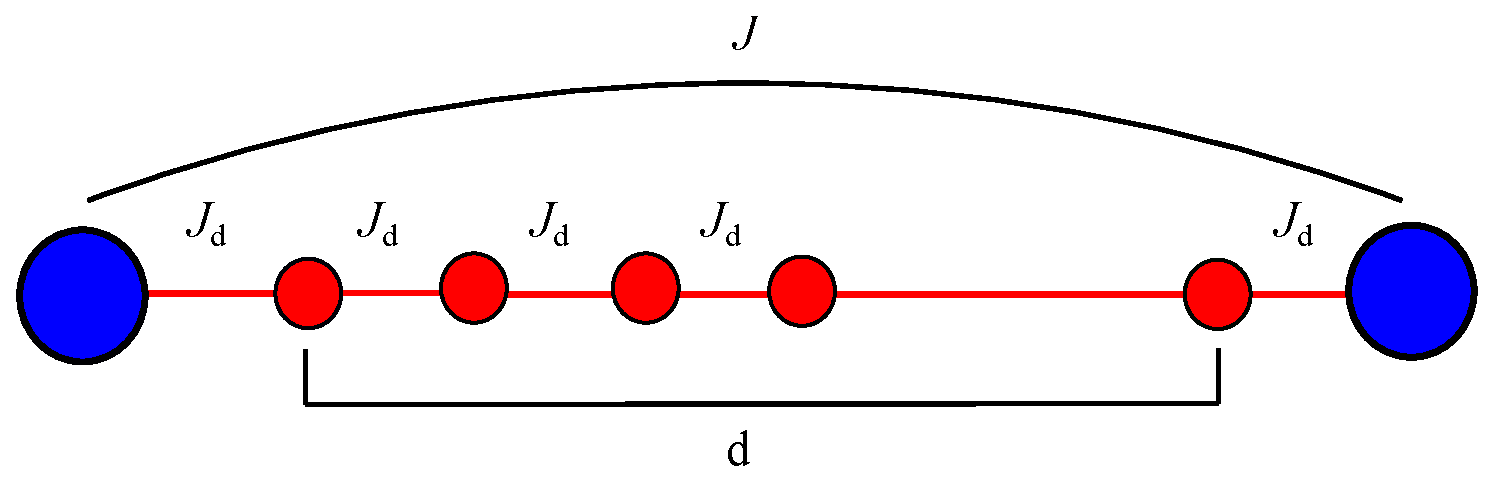
\includegraphics[width=0.7\linewidth]{part3/decorChain.eps}}
 	\caption{Декорированная цепочка с обменным взаимодействием ближайших соседей $J_d$ и обменным взаимодействием $J$}
 	\label{decorChain}
 \end{figure}

На рисунке~\ref{decorChain} изображена решетка спинов, соответствующая декорированной цепочке с гамильтонианом~\eqref{ham}.
Красными кружками обозначены декорационные спины, синими кружками --- основные (нодальные) спины.
Каждый спин обладает двумя состояниями $s=\pm 1$.

Как мы видели, статистическая сумма в термодинамическом пределе ($N\rightarrow \infty$) для единожды декорированной цепочки, то есть при $d=1$, вычисляется из выражения $Z_{N} = \lambda_{\text{max}}^{N/2}$. Статсумма для дважды декорированной цепочки имеет вид $Z_{N} = \lambda_{\text{max}}^{N/3}$, для трижды декорированной цепочки --- $Z_{N} = \lambda_{\text{max}}^{N/4}$ и  т.д. Поэтому легко убедиться в том, что в общем случае выражение для статсуммы с произвольным числом декорирования цепочки примет вид 
\begin{equation}
Z_{N} = \lambda_{\text{max}}^{N/(d+1)}.
\label{zn}
\end{equation}

В формуле \eqref{zn} замечаем, что знаменатель у степени наибольшего собственного значения всегда на единицу больше величины декорирования цепочки $d$. Это означает, что в отсутствие декорационных спинов ($d=0$) цепочка содержит только нодальные спины, таким образом, получаем случай обычной (недекорированной) модели Изинга, статсумма которой вычисляется как $Z_{N} = \lambda_{\text{max}}^{N}$.

Если $d$ устремить к бесконечности, то рассматриваемая задача снова сводится к обычной (недекорированной) модели Изинга, так как при увеличении числа \guillemotleft декораций\guillemotright $ $ относительный вклад в энергию от основных спинов становится все более незначительным.

Согласно алгоритму получения обобщенной трансфер-матрицы Крамерса--Ваннье и применив предложенное Сиози декорационное преобразование (\emph{decoration-iteration transformation})~\cite{siozi_domb1972}, определяем точное выражение для наибольшего собственного значения трансфер-матрицы декорированной цепочки при наличии магнитного поля
\begin{equation}
\lambda_{\text{max}} = \frac{1}{2}\left[e^{\frac{J}{T}}\big(\lambda_1^{d+1} + \lambda_2^{d+1}\big) + e^{-\frac{J}{T}}\big(\lambda_1^{d+1} - \lambda_2^{d+1}\big)\varepsilon \right],
\nonumber
\end{equation}
где 
\begin{align}
\lambda_1 &= \exp{(J_d/T)}[\ch (H/T) + \sqrt{\sh^2 (H/T) + \exp{(-4J_d/T)}}],\nonumber\\
\lambda_2 &= \exp{(J_d/T)}[\ch (H/T) - \sqrt{\sh^2 (H/T) + \exp{(-4J_d/T)}}],\nonumber\\
\varepsilon &= \sqrt{1+\sh^2 (H/T)(\exp(4J/T)-1)/\big(\sh^2 (H/T)+\exp{(-4J_d/T)}\big)}. 	\label{lam}
\end{align}

Термодинамические и магнитные параметры исследуемой декорированной решетки могут быть выражены исключительно через наибольшее собственное значение $\lambda_{\text{max}}$. Тогда, принимая во внимание степень декорирования цепочки $d$, аналитические выражения для энтропии, теплоемкости, намагниченности и параметра порядка, впервые введенного в статье~\cite{kassan-ogly2012}, запишутся следующим образом:
\begin{align}
& S(H,T) = \frac{\ln \lambda_{\text{max}}}{d+1}+\frac{T}{(d+1)\lambda_{\text{max}}}\frac{\partial \lambda_{max}}{\partial T}; \\
& C(H,T) = \frac{T}{(d+1)\lambda_{\text{max}}}\frac{\partial \lambda_{\text{max}}}{\partial T} + \frac{T}{d+1}\frac{\partial }{\partial T}\bigg(\frac{T}{\lambda_{\text{max}}}\frac{\partial \lambda_{\text{max}}}{\partial T}\bigg);\\
& M(H,T) = \frac{T}{(d+1)\lambda_{\text{max}}} \frac{\partial \lambda_{\text{max}}}{\partial H}; \\
& \eta (H,T) = 1-\frac{\ln \lambda_{\text{max}}}{(d+1)\ln 2}-\frac{T}{(d+1)\lambda_{\text{max}} \ln 2}\frac{\partial \lambda_{\text{max}}}{\partial T}.
\end{align} 

\subsection{Термодинамические, магнитные и фрустрационные свойства декорированной изинговской цепочки}

При исследовании модели Изинга на декорированной цепочке в случае антиферромагнитного обмена как между декорационными спинами, так и между основными спинами, в частности, \mbox{$J_d=-1, J=-1$} в магнитном поле $H=2$ при $T\rightarrow 0$, установлено, что энтропию системы (рисунок \ref{entropyDecor}а) можно записать в общем виде для любых значений декорирования $d$
\begin{equation}
\lim_{T \rightarrow 0} S = \frac{1}{d+1} \ln \left[\frac{1}{\sqrt{5}}\left(\varphi^{d+1}-(1-\varphi)^{d+1}\right)\right],
\label{20d}
\end{equation}
где $\varphi=(1+\sqrt{5})/2$ --- золотое сечение.

Таким образом, система в данном режиме фрустрирована, а магнитное поле $H = 2$ является фрустрирующим.

Рисунок \ref{entropyDecor}а демонстрирует, что при стремлении $d$ к бесконечности фрустрирующая энтропия сходится к логарифму золотого сечения. Используя выражение~\eqref{20d}, можно показать, что
\begin{equation}
\lim_{d\rightarrow \infty} \lim_{T \rightarrow 0} S = \lim_{d\rightarrow \infty} \frac{1}{d+1} \ln \left[\frac{1}{\sqrt{5}}\left(\varphi^{d+1}-(1-\varphi)^{d+1}\right)\right] = \ln \varphi.
\label{21d}
\end{equation}

При \mbox{$H=4, J_d=-1, J=-1$} наблюдается еще одно фрустрирующее поле. Фрустрирующая энтропия при разных значениях декорирования (рисунок \ref{entropyDecor}б) представлена в следующем виде
\begin{equation}
\lim_{T \rightarrow 0} S = \frac{1}{d+1} \ln \varphi.
\label{22d}
\end{equation}

 \begin{figure}[h]
 	\begin{minipage}{0.49\linewidth}
 		\center{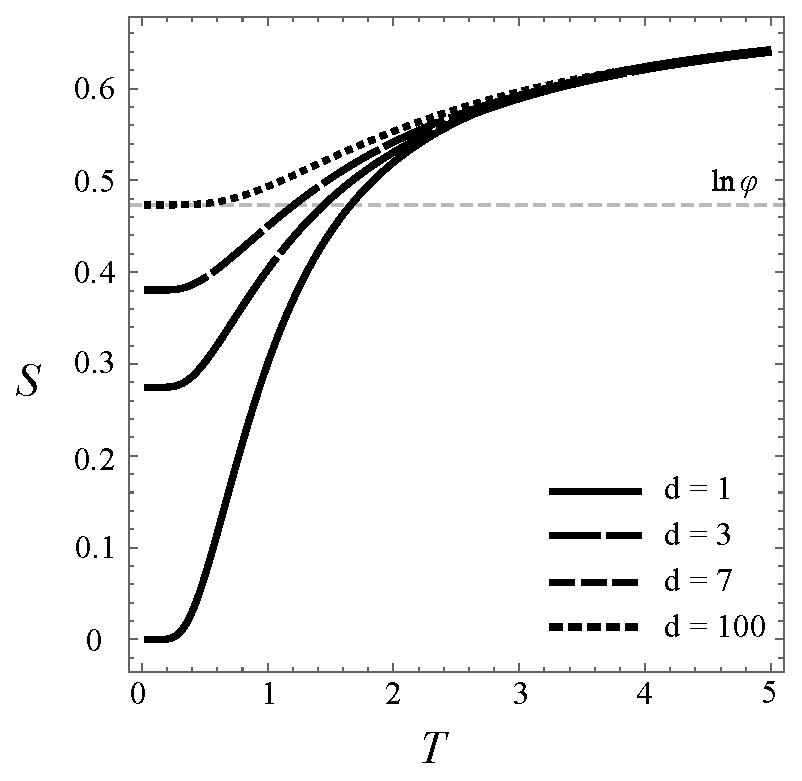
\includegraphics[width=1\linewidth]{part3/entropyDecor1.eps} \\ а)}
 	\end{minipage}
 	\hfill
 	\begin{minipage}{0.49\linewidth}
 		\center{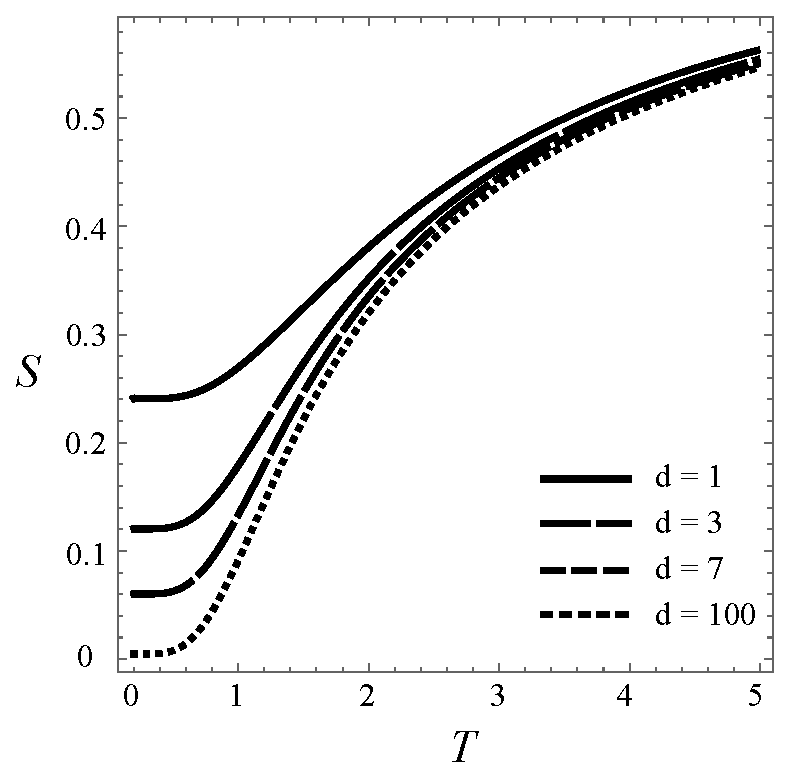
\includegraphics[width=1\linewidth]{part3/entropyDecor2.eps} \\ б)}
 	\end{minipage}
 	\caption{Температурные зависимости энтропий в точках фрустраций антиферромагнитной модели Изинга ($J_d=-1, J=-1$) для различных значений декорирования цепочки: а) в магнитном поле $H=2$;  б) в магнитном поле $H=4$}
 	\label{entropyDecor}
 \end{figure}

Стоит отметить, что при стремлении температуры к бесконечности энтропия равна натуральному логарифму двух 
\begin{equation}
\lim_{T\rightarrow \infty} S = \ln 2,
\label{23d}
\end{equation}
поскольку число состояний на узле равно двум.

Тем не менее, при стремлении температуры к нулю либо к бесконечности теплоемкость при различных параметрах обменных взаимодействий равна нулю (рисунок \ref{heatDecor}а)
\begin{equation}
\lim_{T\rightarrow 0} C = 0,\;\;\;\;\;\;\;\lim_{T\rightarrow \infty} C = 0.
\label{24d}
\end{equation}

Установлено, что в непосредственной близости к точке фрустрации теплоемкость расщепляется на два пика: острый и куполообразный пики. На рисунке \ref{heatDecor}б изображена теплоемкость в точке фрустрации ($H=2$) --- наблюдается единственный куполообразный пик, в то время как в вблизи фрустрации, в частности, в магнитном поле равном $H=1.9$ и $H=2.1$ у теплоемкости появляется дополнительный острый пик. Такое поведение теплоемкости присуще всем фрустрированным системам.

 \begin{figure}[h]
 	\begin{minipage}{0.49\linewidth}
 		\center{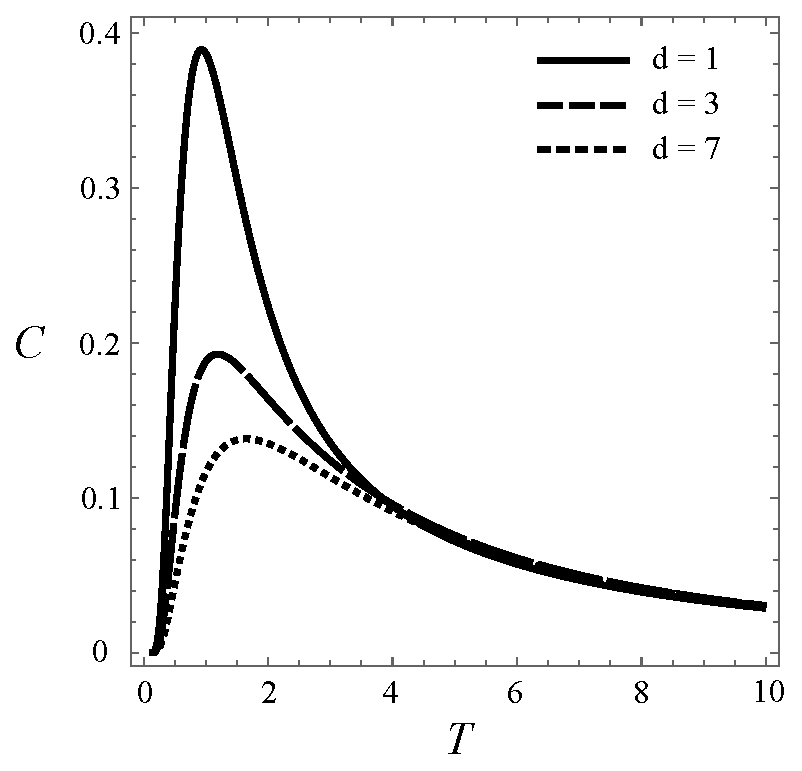
\includegraphics[width=1\linewidth]{part3/heatDecor1.eps} \\ а)}
 	\end{minipage}
 	\hfill
 	\begin{minipage}{0.49\linewidth}
 		\center{\includegraphics[width=1\linewidth]{part3/heatDecor2.eps} \\ б)}
 	\end{minipage}
 	\caption{Температурные зависимости теплоемкостей при различных значениях декорирования $d$: а) теплоемкость всегда при стремлении температуры к нулю или к бесконечности равна нулю ($H=2$ для всех кривых), б) расщепление теплоемкости на два пика вблизи фрустрации}
 	\label{heatDecor}
 \end{figure}

Намагниченность системы в случае антиферромагнитного обмена спинов решетки при $J_d=-1, J=-1$ во фрустрационном поле $H=2$ и при $T\rightarrow 0$ имеет следующие значения при различных кратностях декорирования $d$ (рисунок \ref{magDecor}а)
\begin{equation}
\lim_{T \rightarrow 0} M = \frac{\Big(d+1-\frac{1}{\sqrt{5}}\Big)\varphi^{d+1}+\Big(d+1+\frac{1}{\sqrt{5}}\Big)(1-\varphi)^{d+1}}{\sqrt{5}(d+1)(\varphi^{d+1}-(1-\varphi)^{d+1})}.
\label{25d}
\end{equation}

Во фрустрационном поле $H=4$ в случае антиферромагнитного обмена спинов решетки \mbox{$J_d=-1, J=-1$} и разных параметрах декорирования получаем следующую фрустрирующую намагниченность (рисунок \ref{magDecor}б)
\begin{equation}
\lim_{T \rightarrow 0} M = \frac{1}{\sqrt{5}}\left(\frac{1+d\sqrt{5}}{d+1}\right).
\label{26d}
\end{equation}

Заметим, что характер поведения намагниченности при антиферромагнитном обменном взаимодействии между спинами при нечетных и четных значениях $d$ различен. При нечетных значениях $d$ намагниченность вблизи фрустрирующего поля, равного двум, разделяется на два промежуточных плато (рисунок \ref{magDecor}а), а при четных $d$ происходит образование исключительно только одного промежуточного плато (рисунок \ref{magDecor}б).

 \begin{figure}[h]
 	\begin{minipage}{0.49\linewidth}
 		\center{\includegraphics[width=1\linewidth]{part3/magDecor1.eps} \\ а)}
 	\end{minipage}
 	\hfill
 	\begin{minipage}{0.49\linewidth}
 		\center{\includegraphics[width=1\linewidth]{part3/magDecor2.eps} \\ б)}
 	\end{minipage}
 	\caption{Намагниченность антиферромагнитной модели Изинга ($J_d=-1, J=-1$) для различных значений декорирования цепочки:  а) нечетные значения $d$ при температуре $T=0.06$;  б) четные значения $d$ при температуре $T=0.02$}
 	\label{magDecor}
 \end{figure}

Рассмотрим взаимодействие спинов иного типа, в частности, обмен между декорационными спинами (и между декорационными и основными спинами) $J_d$ определим антиферромагнитным, а обмен между основными (нодальными) спинами $J$ установим ферромагнитным. Графики температурных зависимостей энтропий в точках фрустраций для разных степеней декорирования продемонстрированы на рисунке~\ref{entropyDecor2}.

 \begin{figure}[h]
 	\begin{minipage}{0.49\linewidth}
 		\center{\includegraphics[width=1\linewidth]{part3/entropyDecor3.eps} \\ а)}
 	\end{minipage}
 	\hfill
 	\begin{minipage}{0.49\linewidth}
 		\center{\includegraphics[width=1\linewidth]{part3/entropyDecor4.eps} \\ б)}
 	\end{minipage}
 	\caption{Температурные зависимости энтропий в точках фрустраций антиферро-ферромагнитной модели Изинга ($J_d=-1, J=1$) для различных значений декорирования цепочки: а) в магнитном поле $H=2$;  б) в магнитном поле $H=4$}
 	\label{entropyDecor2}
 \end{figure}

 \begin{figure}[h]
 	\begin{minipage}{0.49\linewidth}
 		\center{\includegraphics[width=1\linewidth]{part3/magDecor3.eps} \\ а)}
 	\end{minipage}
 	\hfill
 	\begin{minipage}{0.46\linewidth}
 		\center{\includegraphics[width=1\linewidth]{part3/magDecor4.eps} \\ б)}
 	\end{minipage}
 	\caption{Намагниченность а) антиферро-ферромагнитной модели Изинга ($J_d=-1$, $J=1$) при температуре $T=0.06$ для четных значений декорирования цепочки;  б) ферро-антиферромагнитной модели Изинга ($J_d=1$, $J=-1$)  при температуре $T=0.06$ для	различных значений декорирования цепочки}
 	\label{magDecor2}
 \end{figure}

При антиферро-ферромагнитном обмене (рисунок \ref{entropyDecor2}а) ($J_d=-1$, $J=1$) во внешнем магнитном поле $H=2$ при $T\rightarrow 0$ фрустрационная энтропия системы выражается следующим образом
\begin{equation}
\lim_{T \rightarrow 0} S = \frac{1}{d+1} \ln \left[\frac{1}{\sqrt{5}}\left(\varphi^{d+2}-(1-\varphi)^{d+2}\right)\right].
\label{27d}
\end{equation}

Соответствующие значения фрустрационных намагниченностей во фрустрационном поле $H=2$ записываются в виде
\begin{equation}
\lim_{T \rightarrow 0} M = \frac{\left(d+2-\frac{1}{\sqrt{5}}\right)\varphi^{d+2}+\left(d+2+\frac{1}{\sqrt{5}}\right)(1-\varphi)^{d+2}}{\sqrt{5}(d+1)(\varphi^{d+2}-(1-\varphi)^{d+2})}.
\label{28d}
\end{equation}

Вместе с тем, во фрустрационном поле $H=4$ замечено, что при различных степенях декорирования решетки, значения фрустрирующих энтропий равны нулю, то есть в этом случае фрустраций не наблюдается, по этой причине, система имеет определенную магнитную конфигурацию в основном состоянии. Этот факт отмечен на рисунке \ref{entropyDecor2}б в случае антиферро-ферромагнитного обмена, помимо этого, на рисунке \ref{magDecor2}а проиллюстрированы намагниченности, описываемые выражениями~\eqref{28d} с фрустрационным полем $H=2$. При четных степенях декорирования $d$ у намагниченности наблюдается только одно промежуточное плато. 

В случае ферро-антиферромагнитного обмена (\mbox{$J_d=1$}, $J\!\!=\!\!-1$), также называемым еще квазиферромагнитным, получаем, что при различных $d$ при сколь угодно малом магнитном поле намагниченность стремится к абсолютному упорядочению вдоль приложенного поля (рисунок \ref{magDecor2}б). 

При ферромагнитном обменном взаимодействии между спинами цепочки ($J_d=1$, $J=1$) при разных значениях параметра $d$ наблюдается подобная ситуация, что и в случае квазиферромагнитного обменного взаимодействия.

Также стоит отметить некоторую особенность поведения намагниченности рассматриваемой декорированной решетки. Установлено, что промежуточные плато намагниченности всегда представляются рациональными дробями. В частности, в случае единожды декорированной цепочки с антиферромагнитным обменом ($J_d=-1$, $J=-1$) имеется промежуточное плато намагниченности со значением $1/2$ (рисунок \ref{magDecor}а), что свидетельствует, что половина спинов развернулось вдоль магнитного поля, в то время как в случае трижды декорированной цепочки плато намагниченностей располагаются на уровнях $1/4$ и $3/4$, и говорят о том, что сначала во фрустрационном поле, равном нулю, повернулась вдоль магнитного поля четверть всех спинов в цепочке, после чего во фрустрационном поле, равном двум, доля повернутых спинов составит три четверти и уже во фрустрационном поле, равном четырем, вдоль магнитного поля развернутся все спины решетки. Несложно определить, что при кратности декорирования, равном $d$, будем иметь плато намагниченности на уровнях $1/(d+1)$ и $d/(d+1)$. А при $d \rightarrow \infty$, замечаем, что промежуточные плато исчезают, а задача сводится к обычной (недекорированной) модели Изинга в магнитном поле с единственным фрустрационным полем равном двум.

 \begin{figure}[h]
 	\center{\includegraphics[width=0.77\linewidth]{part3/thirdDecorHeat.eps}}
 	\caption{Теплоемкость трижды декорированной ($d=3$) антиферромагнитной модели Изинга ($J_d=-1, J=-1$) как функция температуры и магнитного поля}
 	\label{thirdDecorHeat}
 \end{figure}

Приступим к описанию термодинамических и магнитных свойств декорированной изинговской цепочки. Для этого построим трехмерные графики теплоемкости и намагниченности как функций температуры и магнитного поля.

Трехмерный график теплоемкости как функции температуры и магнитного поля для трижды декорированной цепочки в случае антиферромагнитного обмена ($J_d=-1$, $J=-1$) изображен на рисунке~\ref{thirdDecorHeat}. Значения магнитного поля, в точках где теплоемкость обращается в нуль (при $T\rightarrow 0$), соответствуют фрустрационным полям. Замечено, что имеется три фрустрационных поля, равные нулю~(cм. статью~\cite{vakbib2}), двум и четырем. В данных фрустрационных полях намагниченность претерпевает скачок, в чем можно убедиться, глядя на рисунок~\ref{thirdDecorMag}.

 \begin{figure}[h]
 	\center{\includegraphics[width=0.77\linewidth]{part3/thirdDecorMag.eps}}
 	\caption{Намагниченность трижды декорированной ($d=3$) антиферромагнитной модели Изинга ($J_d=-1, J=-1$) как функция температуры и магнитного поля}
 	\label{thirdDecorMag}
 \end{figure}

 \begin{figure}[h]
 	\center{\includegraphics[width=0.7\linewidth]{part3/expMag.eps}}
 	\caption{Экспериментальная намагниченность UThSb~\cite{rossat1982}}
 	\label{expMag}
 \end{figure}

На рисунке~\ref{thirdDecorMag} проиллюстрирован трехмерный график намагниченности как функции температуры и магнитного поля трижды декорированной цепочки в случае антиферромагнитного обмена ($J_d=-1$, $J=-1$). Заметно, что при увеличении температуры кривая намагниченности размывается и промежуточные плато пропадают. 

Можно заметить качественное совпадение между теоретически рассчитанной намагниченностью, изображенной на рисунке~\ref{thirdDecorMag} и полученной экспериментально и проиллюстрированной на рисунке~\ref{expMag}. В обоих случаях имеется ряд скачков намагниченности с низкотемпературными промежуточными плато. При увеличении температуры плато намагниченности также размываются~\cite{rossat1982}. 

 \begin{figure}[h]
 	\begin{minipage}{0.47\linewidth}
 		\center{\includegraphics[width=1\linewidth]{part3/PhaseDiagram1.eps} \\ а)}
 	\end{minipage}
 	\hfill
 	\begin{minipage}{0.47\linewidth}
 		\center{\includegraphics[width=1\linewidth]{part3/PhaseDiagram2.eps} \\ б)}
 	\end{minipage}
 	\caption{Фазовые диаграммы основного состояния системы  декорированной изинговской цепочки в магнитном поле с учетом обменного взаимодействия между ближайшими соседями $J_d=-1$: а) при $d=1$, б) при $d=2$}
 	\label{phaseDiag}
 \end{figure}

Исследуемая декорированная изинговская цепочка зависит от четырех независимых параметров $J_d, J, H, d$, поэтому не представляется возможным изобразить полную фазовую диаграмму, поскольку для этого потребуется четырехмерное пространство. Тем не менее, на рисунке~\ref{phaseDiag} представлены некоторые сечения этого четырехмерного пространства.

Построены магнитные фазовые диаграммы в координатах ($H, J$) для  единожды и дважды декорированной цепочек, находящихся во внешнем магнитном поле (рис.~\ref{phaseDiag}). Замечено, что при $d=1$  в основном состоянии присутствуют три магнитные фазовые конфигурации, а именно, антиферромагнитная фаза $C_2$ с удвоением периода трансляции цепочки 
\begin{equation*}
C_2 =
\left\{\!\begin{aligned}
&\dots \downarrow\;\;\; \uparrow \;\;\;\downarrow \;\;\; \uparrow   \dots\\[1ex]
& \dots \uparrow\;\;\; \downarrow \;\;\;\uparrow \;\;\; \downarrow  \dots
\end{aligned}\right\}
\end{equation*}
с энергией $E_{C_2}^{d=1} = -J/2+J_{d}$, ферромагнитная фаза $C_1$ с сохранением периода трансляции
\begin{equation*}
C_1 =
\left\{\!\begin{aligned}
\dots \uparrow\;\;\; \uparrow \;\;\;\uparrow \;\;\; \uparrow  \dots
\end{aligned}\right\}
\end{equation*}
с энергией $E_{C_1}^{d=1} = -J/2-J_d-H$ и упорядочение $C_4$ с учетверением периода трансляции цепочки 
\begin{equation*}
C_4 =
\left\{\!\begin{aligned}
\dots \uparrow\;\;\; \uparrow \;\;\;\downarrow \;\;\; \uparrow   \dots 
\end{aligned}\right\}
\end{equation*}
с энергией $E_{C_4} = J/2-H/2$ (рисунок~\ref{phaseDiag}a). Все остальные фазы имеют более высокую энергию и оказываются невыгодными в основном состоянии. 

В случае $d=2$ в основном состоянии имеется четыре различных конфигурации: антиферромагнитная $C_2$ с энергией $E_{C_2}^{d=2} = J/3+J_{d}$, ферромагнитная $C_1$ с энергией $E_{C_1}^{d=2} = -J/3-J_d-H$, а также конфигурация $C_3$ c утроением периода трансляции
\begin{equation*}
C_3 =
\left\{\!\begin{aligned}
&\dots \uparrow\;\;\; \uparrow \;\;\;\downarrow   \dots \\[1ex]
&\dots \uparrow\;\;\; \downarrow \;\;\;\uparrow   \dots 
\end{aligned}\right\}
\end{equation*}
с энергией $E_{С_3} = -J/3+J_d/3-H/3$ и фаза $C_6$ с ушестерением периода трансляции
\begin{equation*}
C_6 =
\left\{\!\begin{aligned}
&\dots \uparrow\;\;\; \uparrow \;\;\;\uparrow\;\;\; \downarrow\;\;\; \uparrow \;\;\;\uparrow    \dots \\[1ex]
&\dots \downarrow\;\;\; \uparrow \;\;\;\uparrow\;\;\; \uparrow\;\;\; \uparrow \;\;\;\uparrow    \dots \\[1ex] 
\end{aligned}\right\}
\end{equation*}
с энергией $E_{С_6} = J/3-J_d/3-2H/3$ (рисунок~\ref{phaseDiag}б).

Также, из приведенных диаграмм можно увидеть, что фазы на рисунках сходятся в точке при $J_d=-1, J=0, H=2$. В этой точке схождения фаз нуль-температурная энтропия равняется логарифму золотого сечения, то есть, при таких параметрах задача сводится к обычной (недекорированной) модели Изинга в магнитном поле.

Кроме того, две фазы могут пересекаться на линиях схождения фаз. Такие линии схождения двух фаз, представленные на рисунке~\ref{phaseDiag}, соответствуют определенному обмену --- антиферромагнитному или антиферро-ферромагнитному, которые рассматривались в прошлом разделе. Например, линия схождения фаз $C_1-C_4$ (так же как и $C_1-C_6$) соответствует антиферромагнитному обмену с нуль-температурными энтропиями~\eqref{22} и нуль-температурными намагниченностями~\eqref{26}.

 \begin{figure}[h]
 	\center{\includegraphics[width=0.55\linewidth]{part3/magDecorSquare.eps}}
 	\caption{Намагниченность антиферромагнитной модели Изинга двукратно-, четырехкратно- и шестикратно-декорированной квадратной решетки ($J_{d_x}=-1, J_{d_y}=-1, J_x=-1, J_y=-1$) при $T=0.005$}
 	\label{magDecorSquare}
 \end{figure}

Вместе с тем, наблюдалось соответствие линейной декорированной цепочки с квадратной декорированной решеткой в магнитном поле~\cite{kassan-ogly2020}. Необходимо подчеркнуть, что расчеты намагниченности в настоящем случае одномерной цепочки следовали из точного аналитического решения~\eqref{14}-\eqref{15}, на квадратной решетке это было возможно выполнить лишь трудоемкими численными расчетами, а именно, методом Монте-Карло в алгоритме Ванга -- Ландау~\cite{wang1,wang2}. В качестве примера на рисунке~\ref{magDecorSquare} приведены намагниченности антиферромагнитной модели Изинга двухкратно-, четырехкратно- и шестикратно-декорированной квадратной решетки. Заметно, что на квадратной декорированной решетке появляются два фрустрационных поля при $H=2$ и $H=8$, в отличие от линейной декорированной цепочки при $H=2$ и $H=4$. Помимо этого, можно обнаружить, что возникшие промежуточные плато намагниченностей как в одномерной (плато расположены на уровнях $1/(d+1)$ и $d/(1+d)$), так и двумерной решетках (плато расположены на уровне $(d_x+d_y)/(1+d_x+d_y)$) при $d \rightarrow \infty$ пропадают, а именно происходит скачок намагниченности из антиферромагнитного состояния прямо в ферромагнитное состояние во фрустрационном поле равном двум, следовательно, задача сводится к обычной (недекорированной) модели Изинга. Объясняется это тем, что с увеличением количества декорационных спинов ($d\rightarrow \infty$) влияние нодальных спинов становится все меньше, в равной степени как на одномерной цепочке, так и на квадратной решетке, что напрямую подтверждается рисунками~\ref{magDecor}, \ref{magDecor2} и~\ref{magDecorSquare}.

\section{Выводы по главе}

Полученные результаты по промежуточным плато намагниченности на декорированных решетках могут быть применены для объяснения многих экспериментальных результатов, где наблюдается качественно схожая картина.

Результаты, описанные в этой главе, опубликованы автором в работах~\cite{confbib3, confbib4, confbib5, vakbib2}.

\FloatBarrier           % Глава 3
\chapter*{Заключение}                       % Заголовок
\addcontentsline{toc}{chapter}{Заключение}  % Добавляем его в оглавление

%% Согласно ГОСТ Р 7.0.11-2011:
%% 5.3.3 В заключении диссертации излагают итоги выполненного исследования, рекомендации, перспективы дальнейшей разработки темы.
%% 9.2.3 В заключении автореферата диссертации излагают итоги данного исследования, рекомендации и перспективы дальнейшей разработки темы.
%% Поэтому имеет смысл сделать эту часть общей и загрузить из одного файла в автореферат и в диссертацию:

Основные результаты работы заключаются в следующем.
%% Согласно ГОСТ Р 7.0.11-2011:
%% 5.3.3 В заключении диссертации излагают итоги выполненного исследования, рекомендации, перспективы дальнейшей разработки темы.
%% 9.2.3 В заключении автореферата диссертации излагают итоги данного исследования, рекомендации и перспективы дальнейшей разработки темы.
\begin{enumerate}
  \item На основе анализа \ldots
  \item Численные исследования показали, что \ldots
  \item Математическое моделирование показало \ldots
  \item Для выполнения поставленных задач был создан \ldots
\end{enumerate}

И какая-нибудь заключающая фраза.

Последний параграф может включать благодарности.  В заключение автор
выражает благодарность и большую признательность научному руководителю
Иванову~И.\,И. за поддержку, помощь, обсуждение результатов и~научное
руководство. Также автор благодарит Сидорова~А.\,А. и~Петрова~Б.\,Б.
за помощь в~работе с~образцами, Рабиновича~В.\,В. за предоставленные
образцы и~обсуждение результатов, Занудятину~Г.\,Г. и авторов шаблона
*Russian-Phd-LaTeX-Dissertation-Template* за~помощь в оформлении
диссертации. Автор также благодарит много разных людей
и~всех, кто сделал настоящую работу автора возможной.
      % Заключение
\printnomenclature[3.5cm] % Значение ширины столбца с обозначениями стоит подбирать вручную
        % Список сокращений и условных обозначений
\chapter*{Словарь терминов}             % Заголовок
\addcontentsline{toc}{chapter}{Словарь терминов}  % Добавляем его в оглавление

\textbf{TeX} : Cистема компьютерной вёрстки, разработанная американским профессором информатики Дональдом Кнутом

\textbf{панграмма} : Короткий текст, использующий все или почти все буквы алфавита
      % Словарь терминов
\clearpage                                  % В том числе гарантирует, что список литературы в оглавлении будет с правильным номером страницы
%\hypersetup{ urlcolor=black }               % Ссылки делаем чёрными
%\providecommand*{\BibDash}{}                % В стилях ugost2008 отключаем использование тире как разделителя
\urlstyle{rm}                               % ссылки URL обычным шрифтом
\ifdefmacro{\microtypesetup}{\microtypesetup{protrusion=false}}{} % не рекомендуется применять пакет микротипографики к автоматически генерируемому списку литературы
\insertbibliofull                           % Подключаем Bib-базы: все статьи единым списком
% Режим с подсписками
%\insertbiblioexternal                      % Подключаем Bib-базы: статьи, не являющиеся статьями автора по теме диссертации
% Для вывода выберите и расскомментируйте одно из двух
%\insertbiblioauthor                        % Подключаем Bib-базы: работы автора единым списком 
%\insertbiblioauthorgrouped                 % Подключаем Bib-базы: работы автора сгруппированные (ВАК, WoS, Scopus и т.д.)
\ifdefmacro{\microtypesetup}{\microtypesetup{protrusion=true}}{}
\urlstyle{tt}                               % возвращаем установки шрифта ссылок URL
%\hypersetup{ urlcolor={urlcolor} }          % Восстанавливаем цвет ссылок
      % Список литературы
\clearpage
\ifdefmacro{\microtypesetup}{\microtypesetup{protrusion=false}}{} % не рекомендуется применять пакет микротипографики к автоматически генерируемым спискам
%\listoffigures  % Список изображений

%%% Список таблиц %%%
% (ГОСТ Р 7.0.11-2011, 5.3.10)
\clearpage
%\listoftables   % Список таблиц
\ifdefmacro{\microtypesetup}{\microtypesetup{protrusion=true}}{}
\newpage           % Списки таблиц и изображений (иллюстративный материал)

\setcounter{totalchapter}{\value{chapter}} % Подсчёт количества глав

%%% Настройки для приложений
\appendix
% Оформление заголовков приложений ближе к ГОСТ:
\setlength{\midchapskip}{20pt}
\renewcommand*{\afterchapternum}{\par\nobreak\vskip \midchapskip}
\renewcommand\thechapter{\Asbuk{chapter}} % Чтобы приложения русскими буквами нумеровались

%\chapter{??????? ??????? ????????? ???????????? ????}\label{app:A}

??? ??????? ????????? ???? ??? ???????. ?????? ????????, ?? ? ??? ????? ????
???????? ? ?????????? ????????? (? ??? ????? ??????????? ?~????????????
?~?????????? ??????????), ?? ??????????? ?? ????????~\cref{lst:hwbeauty}.
\begin{ListingEnv}[!h]% ????????? floating ?????????? ????????? figure
    \captiondelim{ } % ??????????? ?????????????? ? ??????? ?? ????????????
    \caption{????????? ,,Hello, world`` ?? \protect\cpp}\label{lst:hwbeauty}
    % ????????? ????????? ??????? ? ????????? ? ????????? ?? ? ?????????? ? ???????????
    \begin{lstlisting}[language={[ISO]C++}]
	#include <iostream>
	using namespace std;

	int main() //????????? ? ???????????? ??? xelatex ? lualatex ????? ???????? ? ?????????
	{
		cout << "Hello, world" << endl; //latin letters in commentaries
		system("pause");
		return 0;
	}
    \end{lstlisting}
\end{ListingEnv}%
?????? ??~????? ????????, ?? ??? ??????????? (??.~???????~\cref{lst:hwplain}).
\begin{ListingEnv}[!h]
    \captiondelim{ } % ??????????? ?????????????? ? ??????? ?? ????????????
    \caption{????????? ,,Hello, world`` ??? ?????????}\label{lst:hwplain}
    \begin{Verb}

        #include <iostream>
        using namespace std;

        int main() //????????? ? ????????????
        {
            cout << "??????, ???" << endl;
        }
    \end{Verb}
\end{ListingEnv}

????? ???????????? ?????? ??? ??????? ????????? ??????????
?????? ??????, ? ?????? ??? ??????? ???????
???? ? ??????????, ???? ??????? ???????.

???? ????? ???????? ?????? ???????? ?????? ???? (???? ??? ??? ??????),
??~?????????  ????????? ? ????????? ????? ?????????? ???????? ?????????.
? ????? ??????? ????? ???????????? ????????? \texttt{lstlisting} ???
\texttt{Verb} ??? \texttt{ListingEnv}. ???????? ????? ??????
? ????????? ????? ????????????????, ????????? ??~????????? ?? ?????????:
\begin{lstlisting}[language=Haskell]
fibs = 0 : 1 : zipWith (+) fibs (tail fibs)
\end{lstlisting}
????? ??????? "--- ?? ???????? ???????????? ????????? ?????????
?~??????? ??? ????????? ??? ????????? ?????????? "--- ???????,
????????, ?~????? ????? ?????????? ? ????? ?????? ?? ???????????
??????????.

???????, ??? ?????????? ??????????????? ?????? ?????
(??????? \lstinline{main} ?~???? ????????) ????????????
\texttt{lstinline} ???, ????? ???????, ???????????? ?????
(\texttt{\textbackslash texttt}).

??????~\cref{lst:internal3}, ?????????????? ??????????? ?????????????????
?????. ????? ???? ????????, ???? ????????? ???? ???????? ?????. ???
??????????????? ?????????, ? ???????? ? ???????, ????????????? ??????????
?????????.
\begingroup
\captiondelim{ } % ??????????? ?????????????? ? ??????? ?? ????????????
\begin{lstlisting}[language={Renhanced},caption={?????? ???????? c ???????? ???????????? ??????????},label={lst:internal3}]
## Caching the Inverse of a Matrix

## Matrix inversion is usually a costly computation and there may be some
## benefit to caching the inverse of a matrix rather than compute it repeatedly
## This is a pair of functions that cache the inverse of a matrix.

## makeCacheMatrix creates a special "matrix" object that can cache its inverse

makeCacheMatrix <- function(x = matrix()) {#????????? ? ???????????? ??? xelatex ? lualatex ????? ???????? ? ?????????
    i <- NULL
    set <- function(y) {
        x <<- y
        i <<- NULL
    }
    get <- function() x
    setSolved <- function(solve) i <<- solve
    getSolved <- function() i
    list(set = set, get = get,
    setSolved = setSolved,
    getSolved = getSolved)

}


## cacheSolve computes the inverse of the special "matrix" returned by
## makeCacheMatrix above. If the inverse has already been calculated (and the
## matrix has not changed), then the cachesolve should retrieve the inverse from
## the cache.

cacheSolve <- function(x, ...) {
    ## Return a matrix that is the inverse of 'x'
    i <- x$getSolved()
    if(!is.null(i)) {
        message("getting cached data")
        return(i)
    }
    data <- x$get()
    i <- solve(data, ...)
    x$setSolved(i)
    i
}
\end{lstlisting} %$ %??????????? ??? ?????????? ????????? ??????????
%??? ????????
\endgroup

???????~\cref{lst:external1} ???????????? ?? ???????? ?????. ??????????
????????? ??? ????????? ???????????????. ????? ?? ????????? ?? ???????????.
\begingroup
\captiondelim{ } % ??????????? ?????????????? ? ??????? ?? ????????????
\lstinputlisting[lastline=78,language={R},caption={??????? ?? ???????? ?????},label={lst:external1}]{listings/run_analysis.R}
\endgroup

\chapter{????? ??????? ???????? ??????? ??????????, ?~??????? ?????????????????? ?????? ?~???????? ?????????}\label{app:B}

\section{????????? ??????????}\label{app:B1}
??? ??????????? ??????? ???????:
\makeatletter
\@ifpackagelater{longtable}{2024/07/04} % hotfix of bug fixed in https://github.com/latex3/latex2e/commit/7c96b6b90a730278903e71a482d88479789a89a3
{% ???? ????? longtable* ???????????? ? ????? latex, ?? ??? ?????? ???? ?????????? ? ??????? ????????? ??????
\renewenvironment{longtable*}
  {\renewcommand\LTcaptype{}\longtable}
  {\endlongtable}
}
{\@ifpackagelater{longtable}{2024/04/26}
    {\addtocounter{table}{-1}}
    {}
}
\makeatother
\fontsize{10pt}{10pt}\selectfont
\begin{longtable*}[c]{|l|c|l|l|} %longtable* ?????????? ?? ?????? ltcaption ? ???? ?????????????? ???????
    \hline
    ???????? & ?????. & ??? & ????????               \\ \hline
    \endfirsthead   \hline
    \multicolumn{4}{|c|}{\small\slshape (???????????)}        \\ \hline
    ???????? & ?????. & ??? & ????????               \\ \hline
    \endhead        \hline
    \multicolumn{4}{|r|}{\small\slshape ??????????? ???????}  \\ \hline
    \endfoot        \hline
    \endlastfoot
    \multicolumn{4}{|l|}{\&INP}        \\ \hline
    kick & 1 & int & 0: ????????????? ??? ???? (\(p_s = const\)) \\
    &   &     & 1: ????????? ?????? ????                  \\
    &   &     & 2: ????????? ?????? ???? ??????????? ???????????? \\
    & & & ????????    \\
    mars & 0 & int & 1: ????????????? ?????? ??? ??????? ????     \\
    kick & 1 & int & 0: ????????????? ??? ???? (\(p_s = const\)) \\
    &   &     & 1: ????????? ?????? ????                  \\
    &   &     & 2: ????????? ?????? ???? ??????????? ???????????? \\
    & & & ????????    \\
    mars & 0 & int & 1: ????????????? ?????? ??? ??????? ????     \\
    kick & 1 & int & 0: ????????????? ??? ???? (\(p_s = const\)) \\
    &   &     & 1: ????????? ?????? ????                  \\
    &   &     & 2: ????????? ?????? ???? ??????????? ???????????? \\
    & & & ????????    \\
    mars & 0 & int & 1: ????????????? ?????? ??? ??????? ????     \\
    kick & 1 & int & 0: ????????????? ??? ???? (\(p_s = const\)) \\
    &   &     & 1: ????????? ?????? ????                  \\
    &   &     & 2: ????????? ?????? ???? ??????????? ???????????? \\
    & & & ????????    \\
    mars & 0 & int & 1: ????????????? ?????? ??? ??????? ????     \\
    kick & 1 & int & 0: ????????????? ??? ???? (\(p_s = const\)) \\
    &   &     & 1: ????????? ?????? ????                  \\
    &   &     & 2: ????????? ?????? ???? ??????????? ???????????? \\
    & & & ????????    \\
    mars & 0 & int & 1: ????????????? ?????? ??? ??????? ????     \\
    kick & 1 & int & 0: ????????????? ??? ???? (\(p_s = const\)) \\
    &   &     & 1: ????????? ?????? ????                  \\
    &   &     & 2: ????????? ?????? ???? ??????????? ???????????? \\
    & & & ????????    \\
    mars & 0 & int & 1: ????????????? ?????? ??? ??????? ????     \\
    kick & 1 & int & 0: ????????????? ??? ???? (\(p_s = const\)) \\
    &   &     & 1: ????????? ?????? ????                  \\
    &   &     & 2: ????????? ?????? ???? ??????????? ???????????? \\
    & & & ????????    \\
    mars & 0 & int & 1: ????????????? ?????? ??? ??????? ????     \\
    kick & 1 & int & 0: ????????????? ??? ???? (\(p_s = const\)) \\
    &   &     & 1: ????????? ?????? ????                  \\
    &   &     & 2: ????????? ?????? ???? ??????????? ???????????? \\
    & & & ????????    \\
    mars & 0 & int & 1: ????????????? ?????? ??? ??????? ????     \\
    kick & 1 & int & 0: ????????????? ??? ???? (\(p_s = const\)) \\
    &   &     & 1: ????????? ?????? ????                  \\
    &   &     & 2: ????????? ?????? ???? ??????????? ???????????? \\
    & & & ????????    \\
    mars & 0 & int & 1: ????????????? ?????? ??? ??????? ????     \\
    kick & 1 & int & 0: ????????????? ??? ???? (\(p_s = const\)) \\
    &   &     & 1: ????????? ?????? ????                  \\
    &   &     & 2: ????????? ?????? ???? ??????????? ???????????? \\
    & & & ????????    \\
    mars & 0 & int & 1: ????????????? ?????? ??? ??????? ????     \\
    kick & 1 & int & 0: ????????????? ??? ???? (\(p_s = const\)) \\
    &   &     & 1: ????????? ?????? ????                  \\
    &   &     & 2: ????????? ?????? ???? ??????????? ???????????? \\
    & & & ????????    \\
    mars & 0 & int & 1: ????????????? ?????? ??? ??????? ????     \\
    kick & 1 & int & 0: ????????????? ??? ???? (\(p_s = const\)) \\
    &   &     & 1: ????????? ?????? ????                  \\
    &   &     & 2: ????????? ?????? ???? ??????????? ???????????? \\
    & & & ????????    \\
    mars & 0 & int & 1: ????????????? ?????? ??? ??????? ????     \\
    kick & 1 & int & 0: ????????????? ??? ???? (\(p_s = const\)) \\
    &   &     & 1: ????????? ?????? ????                  \\
    &   &     & 2: ????????? ?????? ???? ??????????? ???????????? \\
    & & & ????????    \\
    mars & 0 & int & 1: ????????????? ?????? ??? ??????? ????     \\
    kick & 1 & int & 0: ????????????? ??? ???? (\(p_s = const\)) \\
    &   &     & 1: ????????? ?????? ????                  \\
    &   &     & 2: ????????? ?????? ???? ??????????? ???????????? \\
    & & & ????????    \\
    mars & 0 & int & 1: ????????????? ?????? ??? ??????? ????     \\
    kick & 1 & int & 0: ????????????? ??? ???? (\(p_s = const\)) \\
    &   &     & 1: ????????? ?????? ????                  \\
    &   &     & 2: ????????? ?????? ???? ??????????? ???????????? \\
    & & & ????????    \\
    mars & 0 & int & 1: ????????????? ?????? ??? ??????? ????     \\
    \hline
    \multicolumn{4}{|l|}{\&SURFPAR}        \\ \hline
    kick & 1 & int & 0: ????????????? ??? ???? (\(p_s = const\)) \\
    &   &     & 1: ????????? ?????? ????                  \\
    &   &     & 2: ????????? ?????? ???? ??????????? ???????????? \\
    & & & ????????    \\
    mars & 0 & int & 1: ????????????? ?????? ??? ??????? ????     \\
    kick & 1 & int & 0: ????????????? ??? ???? (\(p_s = const\)) \\
    &   &     & 1: ????????? ?????? ????                  \\
    &   &     & 2: ????????? ?????? ???? ??????????? ???????????? \\
    & & & ????????    \\
    mars & 0 & int & 1: ????????????? ?????? ??? ??????? ????     \\
    kick & 1 & int & 0: ????????????? ??? ???? (\(p_s = const\)) \\
    &   &     & 1: ????????? ?????? ????                  \\
    &   &     & 2: ????????? ?????? ???? ??????????? ???????????? \\
    & & & ????????    \\
    mars & 0 & int & 1: ????????????? ?????? ??? ??????? ????     \\
    kick & 1 & int & 0: ????????????? ??? ???? (\(p_s = const\)) \\
    &   &     & 1: ????????? ?????? ????                  \\
    &   &     & 2: ????????? ?????? ???? ??????????? ???????????? \\
    & & & ????????    \\
    mars & 0 & int & 1: ????????????? ?????? ??? ??????? ????     \\
    kick & 1 & int & 0: ????????????? ??? ???? (\(p_s = const\)) \\
    &   &     & 1: ????????? ?????? ????                  \\
    &   &     & 2: ????????? ?????? ???? ??????????? ???????????? \\
    & & & ????????    \\
    mars & 0 & int & 1: ????????????? ?????? ??? ??????? ????     \\
    kick & 1 & int & 0: ????????????? ??? ???? (\(p_s = const\)) \\
    &   &     & 1: ????????? ?????? ????                  \\
    &   &     & 2: ????????? ?????? ???? ??????????? ???????????? \\
    & & & ????????    \\
    mars & 0 & int & 1: ????????????? ?????? ??? ??????? ????     \\
    kick & 1 & int & 0: ????????????? ??? ???? (\(p_s = const\)) \\
    &   &     & 1: ????????? ?????? ????                  \\
    &   &     & 2: ????????? ?????? ???? ??????????? ???????????? \\
    & & & ????????    \\
    mars & 0 & int & 1: ????????????? ?????? ??? ??????? ????     \\
    kick & 1 & int & 0: ????????????? ??? ???? (\(p_s = const\)) \\
    &   &     & 1: ????????? ?????? ????                  \\
    &   &     & 2: ????????? ?????? ???? ??????????? ???????????? \\
    & & & ????????    \\
    mars & 0 & int & 1: ????????????? ?????? ??? ??????? ????     \\
    kick & 1 & int & 0: ????????????? ??? ???? (\(p_s = const\)) \\
    &   &     & 1: ????????? ?????? ????                  \\
    &   &     & 2: ????????? ?????? ???? ??????????? ???????????? \\
    & & & ????????    \\
    mars & 0 & int & 1: ????????????? ?????? ??? ??????? ????     \\
    \hline
\end{longtable*}

\normalsize% ?????????? ????? ? ???????????
\section{??? ???? ????????? ??????????}\label{app:B2}

????? ?????? ??????????? ??????????!
????????? ?????????? ?? ???, ???????? ???????? ????????? ?? ???. ??? ?? ??????
????????, ??? ????? ?????? ???????????? ??, ??? ??????? ???????? ???????? ??.

?????? ??????? ??????? ? ??????? ??????????? ?? ???? 2.105:

\begingroup
\centering
\small
\captionsetup[table]{skip=7pt} % ???????? ????????? ???????
\begin{longtable}[c]{|l|c|l|l|}
    \caption{???????????? ??????? ??????? ?????}\label{tab:test5}% label ?????? ?????????? ???? ????? caption
    \\[-0.45\onelineskip]
    \hline
    ???????? & ?????. & ??? & ????????                                          \\ \hline
    \endfirsthead%
    \caption*{??????????? ???????~\thetable}                                    \\[-0.45\onelineskip]
    \hline
    ???????? & ?????. & ??? & ????????                                          \\ \hline
    \endhead
    \hline
    \endfoot
    \hline
    \endlastfoot
    \multicolumn{4}{|l|}{\&INP}                                                 \\ \hline
    kick     & 1      & int & 0: ????????????? ??? ???? (\(p_s = const\))       \\
             &        &     & 1: ????????? ?????? ????                          \\
             &        &     & 2: ????????? ?????? ???? ??????????? ???????????? \\
             &        &     & ????????                                          \\
    mars     & 0      & int & 1: ????????????? ?????? ??? ??????? ????          \\
    kick     & 1      & int & 0: ????????????? ??? ???? (\(p_s = const\))       \\
             &        &     & 1: ????????? ?????? ????                          \\
             &        &     & 2: ????????? ?????? ???? ??????????? ???????????? \\
             &        &     & ????????                                          \\
    mars     & 0      & int & 1: ????????????? ?????? ??? ??????? ????          \\
    kick     & 1      & int & 0: ????????????? ??? ???? (\(p_s = const\))       \\
             &        &     & 1: ????????? ?????? ????                          \\
             &        &     & 2: ????????? ?????? ???? ??????????? ???????????? \\
             &        &     & ????????                                          \\
    mars     & 0      & int & 1: ????????????? ?????? ??? ??????? ????          \\
    kick     & 1      & int & 0: ????????????? ??? ???? (\(p_s = const\))       \\
             &        &     & 1: ????????? ?????? ????                          \\
             &        &     & 2: ????????? ?????? ???? ??????????? ???????????? \\
             &        &     & ????????                                          \\
    mars     & 0      & int & 1: ????????????? ?????? ??? ??????? ????          \\
    kick     & 1      & int & 0: ????????????? ??? ???? (\(p_s = const\))       \\
             &        &     & 1: ????????? ?????? ????                          \\
             &        &     & 2: ????????? ?????? ???? ??????????? ???????????? \\
             &        &     & ????????                                          \\
    mars     & 0      & int & 1: ????????????? ?????? ??? ??????? ????          \\
    kick     & 1      & int & 0: ????????????? ??? ???? (\(p_s = const\))       \\
             &        &     & 1: ????????? ?????? ????                          \\
             &        &     & 2: ????????? ?????? ???? ??????????? ???????????? \\
             &        &     & ????????                                          \\
    mars     & 0      & int & 1: ????????????? ?????? ??? ??????? ????          \\
    kick     & 1      & int & 0: ????????????? ??? ???? (\(p_s = const\))       \\
             &        &     & 1: ????????? ?????? ????                          \\
             &        &     & 2: ????????? ?????? ???? ??????????? ???????????? \\
             &        &     & ????????                                          \\
    mars     & 0      & int & 1: ????????????? ?????? ??? ??????? ????          \\
    kick     & 1      & int & 0: ????????????? ??? ???? (\(p_s = const\))       \\
             &        &     & 1: ????????? ?????? ????                          \\
             &        &     & 2: ????????? ?????? ???? ??????????? ???????????? \\
             &        &     & ????????                                          \\
    mars     & 0      & int & 1: ????????????? ?????? ??? ??????? ????          \\
    kick     & 1      & int & 0: ????????????? ??? ???? (\(p_s = const\))       \\
             &        &     & 1: ????????? ?????? ????                          \\
             &        &     & 2: ????????? ?????? ???? ??????????? ???????????? \\
             &        &     & ????????                                          \\
    mars     & 0      & int & 1: ????????????? ?????? ??? ??????? ????          \\
    kick     & 1      & int & 0: ????????????? ??? ???? (\(p_s = const\))       \\
             &        &     & 1: ????????? ?????? ????                          \\
             &        &     & 2: ????????? ?????? ???? ??????????? ???????????? \\
             &        &     & ????????                                          \\
    mars     & 0      & int & 1: ????????????? ?????? ??? ??????? ????          \\
    kick     & 1      & int & 0: ????????????? ??? ???? (\(p_s = const\))       \\
             &        &     & 1: ????????? ?????? ????                          \\
             &        &     & 2: ????????? ?????? ???? ??????????? ???????????? \\
             &        &     & ????????                                          \\
    mars     & 0      & int & 1: ????????????? ?????? ??? ??????? ????          \\
    kick     & 1      & int & 0: ????????????? ??? ???? (\(p_s = const\))       \\
             &        &     & 1: ????????? ?????? ????                          \\
             &        &     & 2: ????????? ?????? ???? ??????????? ???????????? \\
             &        &     & ????????                                          \\
    mars     & 0      & int & 1: ????????????? ?????? ??? ??????? ????          \\
    kick     & 1      & int & 0: ????????????? ??? ???? (\(p_s = const\))       \\
             &        &     & 1: ????????? ?????? ????                          \\
             &        &     & 2: ????????? ?????? ???? ??????????? ???????????? \\
             &        &     & ????????                                          \\
    mars     & 0      & int & 1: ????????????? ?????? ??? ??????? ????          \\
    kick     & 1      & int & 0: ????????????? ??? ???? (\(p_s = const\))       \\
             &        &     & 1: ????????? ?????? ????                          \\
             &        &     & 2: ????????? ?????? ???? ??????????? ???????????? \\
             &        &     & ????????                                          \\
    mars     & 0      & int & 1: ????????????? ?????? ??? ??????? ????          \\
    kick     & 1      & int & 0: ????????????? ??? ???? (\(p_s = const\))       \\
             &        &     & 1: ????????? ?????? ????                          \\
             &        &     & 2: ????????? ?????? ???? ??????????? ???????????? \\
             &        &     & ????????                                          \\
    mars     & 0      & int & 1: ????????????? ?????? ??? ??????? ????          \\
    \hline
    \multicolumn{4}{|l|}{\&SURFPAR}                                             \\ \hline
    kick     & 1      & int & 0: ????????????? ??? ???? (\(p_s = const\))       \\
             &        &     & 1: ????????? ?????? ????                          \\
             &        &     & 2: ????????? ?????? ???? ??????????? ???????????? \\
             &        &     & ????????                                          \\
    mars     & 0      & int & 1: ????????????? ?????? ??? ??????? ????          \\
    kick     & 1      & int & 0: ????????????? ??? ???? (\(p_s = const\))       \\
             &        &     & 1: ????????? ?????? ????                          \\
             &        &     & 2: ????????? ?????? ???? ??????????? ???????????? \\
             &        &     & ????????                                          \\
    mars     & 0      & int & 1: ????????????? ?????? ??? ??????? ????          \\
    kick     & 1      & int & 0: ????????????? ??? ???? (\(p_s = const\))       \\
             &        &     & 1: ????????? ?????? ????                          \\
             &        &     & 2: ????????? ?????? ???? ??????????? ???????????? \\
             &        &     & ????????                                          \\
    mars     & 0      & int & 1: ????????????? ?????? ??? ??????? ????          \\
    kick     & 1      & int & 0: ????????????? ??? ???? (\(p_s = const\))       \\
             &        &     & 1: ????????? ?????? ????                          \\
             &        &     & 2: ????????? ?????? ???? ??????????? ???????????? \\
             &        &     & ????????                                          \\
    mars     & 0      & int & 1: ????????????? ?????? ??? ??????? ????          \\
    kick     & 1      & int & 0: ????????????? ??? ???? (\(p_s = const\))       \\
             &        &     & 1: ????????? ?????? ????                          \\
             &        &     & 2: ????????? ?????? ???? ??????????? ???????????? \\
             &        &     & ????????                                          \\
    mars     & 0      & int & 1: ????????????? ?????? ??? ??????? ????          \\
    kick     & 1      & int & 0: ????????????? ??? ???? (\(p_s = const\))       \\
             &        &     & 1: ????????? ?????? ????                          \\
             &        &     & 2: ????????? ?????? ???? ??????????? ???????????? \\
             &        &     & ????????                                          \\
    mars     & 0      & int & 1: ????????????? ?????? ??? ??????? ????          \\
    kick     & 1      & int & 0: ????????????? ??? ???? (\(p_s = const\))       \\
             &        &     & 1: ????????? ?????? ????                          \\
             &        &     & 2: ????????? ?????? ???? ??????????? ???????????? \\
             &        &     & ????????                                          \\
    mars     & 0      & int & 1: ????????????? ?????? ??? ??????? ????          \\
    kick     & 1      & int & 0: ????????????? ??? ???? (\(p_s = const\))       \\
             &        &     & 1: ????????? ?????? ????                          \\
             &        &     & 2: ????????? ?????? ???? ??????????? ???????????? \\
             &        &     & ????????                                          \\
    mars     & 0      & int & 1: ????????????? ?????? ??? ??????? ????          \\
    kick     & 1      & int & 0: ????????????? ??? ???? (\(p_s = const\))       \\
             &        &     & 1: ????????? ?????? ????                          \\
             &        &     & 2: ????????? ?????? ???? ??????????? ???????????? \\
             &        &     & ????????                                          \\
    mars     & 0      & int & 1: ????????????? ?????? ??? ??????? ????          \\
\end{longtable}
\normalsize% ?????????? ????? ? ???????????
\endgroup
\section{????????????? ??????? ?????? ? ?????????? \textit{longtblr} ??~?????? \texttt{tabularray}}\label{app:B2a}

? ??????? \cref{tab:test-functions} ????? ??????? ??????? ??????? ???????,
????????? ????????? \verb!longtblr! ??~?????? \verb!tabularray! ? ?????????????
??????????? (\verb!toprule!, \verb!midrule!, \verb!bottomrule!) ??~??????
\verb!booktabs!.

????? ????????? ??????? ?????????? ?????, ????? ???????????? ?????????
?????????.
??????? ???????? ?? ??? ??????, \verb!longtblr! ????????? ?????? ?????? ???????
??????????????? "--- ??? ??? ??????? ?~????????? 1.1:1.1:4 "--- ??? ??????
??????? ?????? ???????? ?~???????? \verb!X[]!.
????? ????, ?~??????? ?????? ??????? ????? ? ?????? ?~??????? \verb!@{}!
?~????????? ???????.
?~??????? ?~??????? ??????? ??????????? ???????????

\verb!>{\setlength{\baselineskip}{0.7\baselineskip}}!,

\noindent ??????? ????????? ??????????? ???????? ??? ?????? ?????? (?????
????????? ??????? ??????? ??????????? ????, ? ???????????? ???
????????? ?~???????????). ??? ?????? ? ?????? ??????? ????? ? ???????
????????????? ??~?????? ??? ??~?????????, ??? ? ?? ??????????? "---
???????? ??????? \verb!m!~?~\verb!c!~?~???????? ??????? \verb!X[]!.

??? ??? ??????? ??????? "--- ???????????? ????????? \verb!alignedat!,
????? ?????? ??? ?????????? ? ???? ?????? "--- ?? ?????? ??? ????, ????
??? ??????? ????? ????? ???? ? ?? ????????????.  ????? ???????
???????? ???????? ????? ?~?????? ??????? ??????? (??? ????)
???????????? \verb!\textstyle! "--- ??~?????? ????? ??????, ?~??????
????? ? ???????????? "--- ??????? ?????. ?????? ??????? ??????? ???????,
????????? ?? ?????????, ??????? ????? ??? ???????? ?????????
?????????????? ?????? \verb!\vspace*{2ex}!. ??? ???????? ??????? "---
?????? ???????? ?????? ????? ??????? \verb!\Big\{!, ?.\:?. ??~?????
\verb!alignedat! ???????? ?~\verb!\left! ?~\verb!\right! ?????
????????? ?????/???????.

? ?????????? ? ??????? ????????, ????????? \verb!cases! ???? ???????
??????? ?????????? ????? ??????????, ????? ?? ?????????, ? ?????
?????? ??????? ????????? ????????????? ????????????? ??????????????
?????? \verb!\\[-0.5em]!.

\DefTblrTemplate{contfoot-text}{default}{\small\slshape ??????????? ???????} % ?????????? default ??????, ???????????? ??-?????????
\DefTblrTemplate{conthead-text}{default}{\small\slshape (???????????)} % ?????????? normal default, ???????????? ??-?????????
\DefTblrTemplate{capcont}{default}{\centering\UseTblrTemplate{conthead-text}{default}\par} % ??? ?????? ????????????? ??????????? \par
\DefTblrTemplate{caplast}{default}{\small\slshape (?????????)}
\DefTblrTemplate{lasthead}{default}{\centering\UseTblrTemplate{caplast}{default}\par} % ??? ?????? ????????????? ??????????? \par
\DefTblrTemplate{firsthead}{default}{% ?????? ?????? ? ??????? ?????????, ????? ???????? ????????? ?? ?????? caption
    % https://tex.stackexchange.com/a/628973
    \addtocounter{table}{-1}%
    \IfTokenListEmpty{\InsertTblrText{entry}}{% ?????, ????? ?? ????????????? ?????? ? ?????? ??????
        \captionof{table}{\InsertTblrText{caption}}%
    }{%
        \captionof{table}[\InsertTblrText{entry}]{\InsertTblrText{caption}}%
    }% ???? ????? ?????? ? entry, ?? ??? ?????? ? ?????? ??????, ??. ???????????? tabularray
}
\SetTblrTemplate{caption-lot}{empty} % ?????, ????? ?? ????????????? ?????? ? ?????? ??????
\begin{longtblr}[
    caption = {???????? ??????? ??? ???????????, \(D\) "---  ???????????. ??? ???? ??????? ???????? ? ????? ??????????? ???????? ????? ????.},
    label = {tab:test-functions},
    ]{
    colspec = {%
    @{}>{\setlength{\baselineskip}{0.7\baselineskip}}X[1.1,m,c]%
    >{\setlength{\baselineskip}{0.7\baselineskip}}X[1.1,m,c]%
    X[4,l]@{}%
    },
    width = \textwidth,
    rowhead = 1,
    rows={rowsep=3pt},
    row{1}={rowsep=2pt},
    }
    \toprule     %%% ??????? ???????
    ???                      & ????????? ???????? ??????????   & ???????                                 \\
    \midrule %%% ?????? ???????????. ???????? ???????? ????????. ?????????? ?? ???? 2.105 ????? 4.4.5
    ?????                    & \(\left[-100,\,100\right]^D\)   &
    \(\begin{aligned}
          \textstyle f_1(x)=\sum_{i=1}^Dx_i^2
      \end{aligned}\)                                                                 \\
    Schwefel 2.22            & \(\left[-10,\,10\right]^D\)     &
    \(\begin{aligned}
          \textstyle f_2(x)=\sum_{i=1}^D|x_i|+\prod_{i=1}^D|x_i|
      \end{aligned}\)                                              \\
    Schwefel 1.2             & \(\left[-100,\,100\right]^D\)   &
    \(\begin{aligned}
          \textstyle f_3(x)=\sum_{i=1}^D\left(\sum_{j=1}^ix_j\right)^2
      \end{aligned}\)                            \\
    Schwefel 2.21            & \(\left[-100,\,100\right]^D\)   &
    \(\begin{aligned}
          \textstyle f_4(x)=\max_i\!\left\{\left|x_i\right|\right\}
      \end{aligned}\)                                           \\
    Rosenbrock               & \(\left[-30,\,30\right]^D\)     &
    \(\begin{aligned}
          \textstyle f_5(x)=
          \sum_{i=1}^{D-1}
          \left[100\!\left(x_{i+1}-x_i^2\right)^2+(x_i-1)^2\right]
      \end{aligned}\)                      \\
    ???????????              & \(\left[-100,\,100\right]^D\)   &
    \(\begin{aligned}
          \textstyle f_6(x)=\sum_{i=1}^D\big\lfloor x_i+0.5\big\rfloor^2
      \end{aligned}\)                                      \\
    ??????????? ???????????? & \(\left[-1.28,\,1.28\right]^D\) &
    \(\begin{aligned}
          \textstyle f_7(x)=\sum_{i=1}^Dix_i^4+rand[0,1)
      \end{aligned}\)\vspace*{2ex}                                                      \\
    Schwefel 2.26            & \(\left[-500,\,500\right]^D\)   &
    \(\begin{aligned}
          f_8(x)= & \textstyle\sum_{i=1}^D-x_i\,\sin\sqrt{|x_i|}\,+ \\
                  & \vphantom{\sum}+ D\cdot
          418.98288727243369
      \end{aligned}\)                                          \\
    Rastrigin                & \(\left[-5.12,\,5.12\right]^D\) &
    \(\begin{aligned}
          \textstyle f_9(x)=\sum_{i=1}^D\left[x_i^2-10\,\cos(2\pi x_i)+10\right]
      \end{aligned}\)\vspace*{2ex}                              \\
    Ackley                   & \(\left[-32,\,32\right]^D\)     &
    \(\begin{aligned}
          f_{10}(x)= & \textstyle -20\, \exp\!\left(
          -0.2\sqrt{\frac{1}{D}\sum_{i=1}^Dx_i^2} \right)- \\
                     & \textstyle - \exp\left(
              \frac{1}{D}\sum_{i=1}^D\cos(2\pi x_i)  \right)
          + 20 + e
      \end{aligned}\)                               \\
    Griewank                 & \(\left[-600,\,600\right]^D\)   &
    \(\begin{aligned}
          f_{11}(x)= & \textstyle \frac{1}{4000}\sum_{i=1}^{D}x_i^2 -
          \prod_{i=1}^D\cos\left(x_i/\sqrt{i}\right) +1
      \end{aligned}\) \vspace*{3ex}                                        \\
    ???????? 1               & \(\left[-50,\,50\right]^D\)     &
    \(\begin{aligned}
          f_{12}(x)= & \textstyle \frac{\pi}{D}\Big\{ 10\,\sin^2(\pi y_1) +            \\
                     & +\textstyle \sum_{i=1}^{D-1}(y_i-1)^2
          \left[1+10\,\sin^2(\pi y_{i+1})\right] +                                     \\
                     & +(y_D-1)^2 \Big\} +\textstyle\sum_{i=1}^D u(x_i,\,10,\,100,\,4)
      \end{aligned}\) \vspace*{2ex} \\
    ???????? 2               & \(\left[-50,\,50\right]^D\)     &
    \(\begin{aligned}
          f_{13}(x)= & \textstyle 0.1 \Big\{\sin^2(3\pi x_1) +            \\
                     & +\textstyle \sum_{i=1}^{D-1}(x_i-1)^2
          \left[1+\sin^2(3 \pi x_{i+1})\right] +                          \\
                     & +(x_D-1)^2\left[1+\sin^2(2\pi x_D)\right] \Big\} + \\
                     & +\textstyle\sum_{i=1}^D u(x_i,\,5,\,100,\,4)
      \end{aligned}\)              \\
    ?????                    & \(\left[-100,\,100\right]^D\)   &
    \(\begin{aligned}
          \textstyle f_1(x)=\sum_{i=1}^Dx_i^2
      \end{aligned}\)                                                                 \\
    Schwefel 2.22            & \(\left[-10,\,10\right]^D\)     &
    \(\begin{aligned}
          \textstyle f_2(x)=\sum_{i=1}^D|x_i|+\prod_{i=1}^D|x_i|
      \end{aligned}\)                                              \\
    Schwefel 1.2             & \(\left[-100,\,100\right]^D\)   &
    \(\begin{aligned}
          \textstyle f_3(x)=\sum_{i=1}^D\left(\sum_{j=1}^ix_j\right)^2
      \end{aligned}\)                            \\
    Schwefel 2.21            & \(\left[-100,\,100\right]^D\)   &
    \(\begin{aligned}
          \textstyle f_4(x)=\max_i\!\left\{\left|x_i\right|\right\}
      \end{aligned}\)                                           \\
    Rosenbrock               & \(\left[-30,\,30\right]^D\)     &
    \(\begin{aligned}
          \textstyle f_5(x)=
          \sum_{i=1}^{D-1}
          \left[100\!\left(x_{i+1}-x_i^2\right)^2+(x_i-1)^2\right]
      \end{aligned}\)                      \\
    ???????????              & \(\left[-100,\,100\right]^D\)   &
    \(\begin{aligned}
          \textstyle f_6(x)=\sum_{i=1}^D\big\lfloor x_i+0.5\big\rfloor^2
      \end{aligned}\)                                      \\
    ??????????? ???????????? & \(\left[-1.28,\,1.28\right]^D\) &
    \(\begin{aligned}
          \textstyle f_7(x)=\sum_{i=1}^Dix_i^4+rand[0,1)
      \end{aligned}\)\vspace*{2ex}                                                      \\
    Schwefel 2.26            & \(\left[-500,\,500\right]^D\)   &
    \(\begin{aligned}
          f_8(x)= & \textstyle\sum_{i=1}^D-x_i\,\sin\sqrt{|x_i|}\,+ \\
                  & \vphantom{\sum}+ D\cdot
          418.98288727243369
      \end{aligned}\)                                          \\
    Rastrigin                & \(\left[-5.12,\,5.12\right]^D\) &
    \(\begin{aligned}
          \textstyle f_9(x)=\sum_{i=1}^D\left[x_i^2-10\,\cos(2\pi x_i)+10\right]
      \end{aligned}\)\vspace*{2ex}                              \\
    Ackley                   & \(\left[-32,\,32\right]^D\)     &
    \(\begin{aligned}
          f_{10}(x)= & \textstyle -20\, \exp\!\left(
          -0.2\sqrt{\frac{1}{D}\sum_{i=1}^Dx_i^2} \right)- \\
                     & \textstyle - \exp\left(
              \frac{1}{D}\sum_{i=1}^D\cos(2\pi x_i)  \right)
          + 20 + e
      \end{aligned}\)                               \\
    Griewank                 & \(\left[-600,\,600\right]^D\)   &
    \(\begin{aligned}
          f_{11}(x)= & \textstyle \frac{1}{4000}\sum_{i=1}^{D}x_i^2 -
          \prod_{i=1}^D\cos\left(x_i/\sqrt{i}\right) +1
      \end{aligned}\) \vspace*{3ex}                                        \\
    ???????? 1               & \(\left[-50,\,50\right]^D\)     &
    \(\begin{aligned}
          f_{12}(x)= & \textstyle \frac{\pi}{D}\Big\{ 10\,\sin^2(\pi y_1) +            \\
                     & +\textstyle \sum_{i=1}^{D-1}(y_i-1)^2
          \left[1+10\,\sin^2(\pi y_{i+1})\right] +                                     \\
                     & +(y_D-1)^2 \Big\} +\textstyle\sum_{i=1}^D u(x_i,\,10,\,100,\,4)
      \end{aligned}\) \vspace*{2ex} \\
    ???????? 2               & \(\left[-50,\,50\right]^D\)     &
    \(\begin{aligned}
          f_{13}(x)= & \textstyle 0.1 \Big\{\sin^2(3\pi x_1) +            \\
                     & +\textstyle \sum_{i=1}^{D-1}(x_i-1)^2
          \left[1+\sin^2(3 \pi x_{i+1})\right] +                          \\
                     & +(x_D-1)^2\left[1+\sin^2(2\pi x_D)\right] \Big\} + \\
                     & +\textstyle\sum_{i=1}^D u(x_i,\,5,\,100,\,4)
      \end{aligned}\)              \\
    \midrule%%% ?????? ???????????
    \SetCell[c=3]{l,\linewidth}%
    \hspace*{2.5em}% ???????? ?????? - ?????????? ???? 2.105
    ?????????? "---  ??? ??????? \(f_{12}\) ? \(f_{13}\)
    ???????????? \(y_i = 1 + \frac{1}{4}(x_i+1)\)
    ?~\(u(x_i,\,a,\,k,\,m)=
    \begin{cases*}
        k(x_i-a)^m,  & \( x_i >a \)            \\[-0.5em]
        0,           & \( -a\leq x_i \leq a \) \\[-0.5em]
        k(-x_i-a)^m, & \( x_i <-a \)
    \end{cases*}
    \)                                                                                                   \\
    \bottomrule %%% ?????? ???????
\end{longtblr}

\section{?????????????? ?????? ??????}\label{app:B3}

? ??????? \cref{tab:other-row} ?????? ? ????????????? ???????????????.
??? ??????????? ??????????, ?????????? ? ???????? ?????? \verb+tabularray+.

? ??????? \cref{tab:other-row} ?????? ?????? ??????? (????????? ??????? ????
????????? ??~???????) "--- ?????, ???????? "--- ? ???????? ?~?????? ???????
?????.
????????? ??? ???????? ? ????, ??? ??????? ???????? ?~??????????????????
????????? ???????????? ? ?????? ?????????? ???????? ?~???????.
??????????? ??????????? ????????? ???????? ? ??????? ???????? ?????? ???
???????.
?~??????? ?~??????? ??????? ?????????????? ?? ??????????? ??~???? ???????,
?~??????? ????? ?????????????? ??~??????????? ??? ???????????.

\needspace{2\baselineskip}
\begin{longtblr}[
    caption = {??????? ??????? ? ???????? ?????????????? ??????????????},
    label = {tab:other-row},
    ]{
    vspan=minimal,
    stretch=0,
    rows={m,ht=0.8\baselineskip},
    columns={c},
    colspec = {%
    @{}X[0.27,l]%
    @{}X[0.7]%
    @{}X%
    @{}X%
    @{}X%
    @{}X[0.98]%
    @{}X[preto={\setlength{\baselineskip}{0.7\baselineskip}}]%
    @{}X@{}%
    },
    width = \textwidth,
    rowhead = 1,
    cell{even}{3-5,7-8} = {font=\color{blue}},
    cell{odd[3]}{3-5,7-8} = {cmd={\vspace{0.3ex}},font=\itshape},
        }
    \toprule %%% ??????? ???????
        & ?????\-??? & JADE\texttt{++}  & JADE      & jDE                    & SaDE                   & DE/rand /1/bin & PSO       \\
    \midrule %%% ?????? ???????????. ???????? ???????? ????????. ?????????? ?? ???? 2.105 ????? 4.4.5
    f1  & 1500       & \textbf{1.8E-60} & 1.3E-54   & 2.5E-28                & 4.5E-20                & 9.8E-14        & 9.6E-42   \\\nopagebreak
        &            & (8.4E-60)        & (9.2E-54) & {\color{red}(3.5E-28)} & (6.9E-20)              & (8.4E-14)      & (2.7E-41) \\
    f2  & 2000       & 1.8E-25          & 3.9E-22   & 1.5E-23                & 1.9E-14                & 1.6E-09        & 9.3E-21   \\\nopagebreak
        &            & (8.8E-25)        & (2.7E-21) & (1.0E-23)              & (1.1E-14)              & (1.1E-09)      & (6.3E-20) \\
    f3  & 5000       & 5.7E-61          & 6.0E-87   & 5.2E-14                & {\color{green}9.0E-37} & 6.6E-11        & 2.5E-19   \\\nopagebreak
        &            & (2.7E-60)        & (1.9E-86) & (1.1E-13)              & (5.4E-36)              & (8.8E-11)      & (3.9E-19) \\
    f4  & 5000       & 8.2E-24          & 4.3E-66   & 1.4E-15                & 7.4E-11                & 4.2E-01        & 4.4E-14   \\\nopagebreak
        &            & (4.0E-23)        & (1.2E-65) & (1.0E-15)              & (1.8E-10)              & (1.1E+00)      & (9.3E-14) \\
    f5  & 3000       & 8.0E-02          & 3.2E-01   & 1.3E+01                & 2.1E+01                & 2.1E+00        & 2.5E+01   \\\nopagebreak
        &            & (5.6E-01)        & (1.1E+00) & (1.4E+01)              & (7.8E+00)              & (1.5E+00)      & (3.2E+01) \\
    f6  & 100        & 2.9E+00          & 5.6E+00   & 1.0E+03                & 9.3E+02                & 4.7E+03        & 4.5E+01   \\\nopagebreak
        &            & (1.2E+00)        & (1.6E+00) & (2.2E+02)              & (1.8E+02)              & (1.1E+03)      & (2.4E+01) \\
    f7  & 3000       & 6.4E-04          & 6.8E-04   & 3.3E-03                & 4.8E-03                & 4.7E-03        & 2.5E-03   \\\nopagebreak
        &            & (2.5E-04)        & (2.5E-04) & (8.5E-04)              & (1.2E-03)              & (1.2E-03)      & (1.4E-03) \\
    f8  & 1000       & 3.3E-05          & 7.1E+00   & 7.9E-11                & 4.7E+00                & 5.9E+03        & 2.4E+03   \\\nopagebreak
        &            & (2.3E-05)        & (2.8E+01) & (1.3E-10)              & (3.3E+01)              & (1.1E+03)      & (6.7E+02) \\
    f9  & 1000       & 1.0E-04          & 1.4E-04   & 1.5E-04                & 1.2E-03                & 1.8E+02        & 5.2E+01   \\\nopagebreak
        &            & (6.0E-05)        & (6.5E-05) & (2.0E-04)              & (6.5E-04)              & (1.3E+01)      & (1.6E+01) \\
    f10 & 500        & 8.2E-10          & 3.0E-09   & 3.5E-04                & 2.7E-03                & 1.1E-01        & 4.6E-01   \\\nopagebreak
        &            & (6.9E-10)        & (2.2E-09) & (1.0E-04)              & (5.1E-04)              & (3.9E-02)      & (6.6E-01) \\
    f11 & 500        & 9.9E-08          & 2.0E-04   & 1.9E-05                & 7.8E-04                & 2.0E-01        & 1.3E-02   \\\nopagebreak
        &            & (6.0E-07)        & (1.4E-03) & (5.8E-05)              & (1.2E-03)              & (1.1E-01)      & (1.7E-02) \\
    f12 & 500        & 4.6E-17          & 3.8E-16   & 1.6E-07                & 1.9E-05                & 1.2E-02        & 1.9E-01   \\\nopagebreak
        &            & (1.9E-16)        & (8.3E-16) & (1.5E-07)              & (9.2E-06)              & (1.0E-02)      & (3.9E-01) \\
    f13 & 500        & 2.0E-16          & 1.2E-15   & 1.5E-06                & 6.1E-05                & 7.5E-02        & 2.9E-03   \\\nopagebreak
        &            & (6.5E-16)        & (2.8E-15) & (9.8E-07)              & (2.0E-05)              & (3.8E-02)      & (4.8E-03) \\
    f1  & 1500       & \textbf{1.8E-60} & 1.3E-54   & 2.5E-28                & 4.5E-20                & 9.8E-14        & 9.6E-42   \\\nopagebreak
        &            & (8.4E-60)        & (9.2E-54) & {\color{red}(3.5E-28)} & (6.9E-20)              & (8.4E-14)      & (2.7E-41) \\
    f2  & 2000       & 1.8E-25          & 3.9E-22   & 1.5E-23                & 1.9E-14                & 1.6E-09        & 9.3E-21   \\\nopagebreak
        &            & (8.8E-25)        & (2.7E-21) & (1.0E-23)              & (1.1E-14)              & (1.1E-09)      & (6.3E-20) \\
    f3  & 5000       & 5.7E-61          & 6.0E-87   & 5.2E-14                & 9.0E-37                & 6.6E-11        & 2.5E-19   \\\nopagebreak
        &            & (2.7E-60)        & (1.9E-86) & (1.1E-13)              & (5.4E-36)              & (8.8E-11)      & (3.9E-19) \\
    f4  & 5000       & 8.2E-24          & 4.3E-66   & 1.4E-15                & 7.4E-11                & 4.2E-01        & 4.4E-14   \\\nopagebreak
        &            & (4.0E-23)        & (1.2E-65) & (1.0E-15)              & (1.8E-10)              & (1.1E+00)      & (9.3E-14) \\
    f5  & 3000       & 8.0E-02          & 3.2E-01   & 1.3E+01                & 2.1E+01                & 2.1E+00        & 2.5E+01   \\\nopagebreak
        &            & (5.6E-01)        & (1.1E+00) & (1.4E+01)              & (7.8E+00)              & (1.5E+00)      & (3.2E+01) \\
    f6  & 100        & 2.9E+00          & 5.6E+00   & 1.0E+03                & 9.3E+02                & 4.7E+03        & 4.5E+01   \\\nopagebreak
        &            & (1.2E+00)        & (1.6E+00) & (2.2E+02)              & (1.8E+02)              & (1.1E+03)      & (2.4E+01) \\
    f7  & 3000       & 6.4E-04          & 6.8E-04   & 3.3E-03                & 4.8E-03                & 4.7E-03        & 2.5E-03   \\\nopagebreak
        &            & (2.5E-04)        & (2.5E-04) & (8.5E-04)              & (1.2E-03)              & (1.2E-03)      & (1.4E-03) \\
    f8  & 1000       & 3.3E-05          & 7.1E+00   & 7.9E-11                & 4.7E+00                & 5.9E+03        & 2.4E+03   \\\nopagebreak
        &            & (2.3E-05)        & (2.8E+01) & (1.3E-10)              & (3.3E+01)              & (1.1E+03)      & (6.7E+02) \\
    f9  & 1000       & 1.0E-04          & 1.4E-04   & 1.5E-04                & 1.2E-03                & 1.8E+02        & 5.2E+01   \\\nopagebreak
        &            & (6.0E-05)        & (6.5E-05) & (2.0E-04)              & (6.5E-04)              & (1.3E+01)      & (1.6E+01) \\
    f10 & 500        & 8.2E-10          & 3.0E-09   & 3.5E-04                & 2.7E-03                & 1.1E-01        & 4.6E-01   \\\nopagebreak
        &            & (6.9E-10)        & (2.2E-09) & (1.0E-04)              & (5.1E-04)              & (3.9E-02)      & (6.6E-01) \\
    f11 & 500        & 9.9E-08          & 2.0E-04   & 1.9E-05                & 7.8E-04                & 2.0E-01        & 1.3E-02   \\\nopagebreak
        &            & (6.0E-07)        & (1.4E-03) & (5.8E-05)              & (1.2E-03)              & (1.1E-01)      & (1.7E-02) \\
    f12 & 500        & 4.6E-17          & 3.8E-16   & 1.6E-07                & 1.9E-05                & 1.2E-02        & 1.9E-01   \\\nopagebreak
        &            & (1.9E-16)        & (8.3E-16) & (1.5E-07)              & (9.2E-06)              & (1.0E-02)      & (3.9E-01) \\
    f13 & 500        & 2.0E-16          & 1.2E-15   & 1.5E-06                & 6.1E-05                & 7.5E-02        & 2.9E-03   \\\nopagebreak
        &            & (6.5E-16)        & (2.8E-15) & (9.8E-07)              & (2.0E-05)              & (3.8E-02)      & (4.8E-03) \\
    \bottomrule %%% ?????? ???????
\end{longtblr}

\section{??????????? ???????? ??????}\label{app:B4}

???????????? ???????? ????????? ?????? ??????: \texttt{<prefix>:<label>}.
????????, \verb+\label{fig:knuth}+; \verb+\ref{tab:test1}+; \verb+label={lst:external1}+.
?~??????? \cref{tab:tab_pref} ????????? ??????????? ???????? ??? ?????????
????? ??????.

\begin{table}[htbp]
    \captionsetup{justification=centering}
    \centering{
        \caption{\label{tab:tab_pref}??????????? ???????? ??????}
        \begin{tabular}{ll}
            \toprule
            \textbf{???????} & \textbf{????????} \\
            \midrule
            ch:              & ?????             \\
            sec:             & ??????            \\
            subsec:          & ?????????         \\
            fig:             & ???????           \\
            tab:             & ???????           \\
            eq:              & ?????????         \\
            lst:             & ??????? ????????? \\
            itm:             & ??????? ??????    \\
            alg:             & ????????          \\
            app:             & ?????? ?????????? \\
            \bottomrule
        \end{tabular}
    }
\end{table}


??? ?????????????? ?????? ????? ???????????? ?????????????? ???????.
????????, \verb+\label{fig:scheemes/my_scheeme}+ ??? \\ \verb+\label{lst:dts/linked_list}+.

\section{????????? ????????? ??????????}\label{app:B5}

????? ?????? ??????????? ??????????!

\section{? ??? ???? ????????? ??????????}\label{app:B6}

????? ?????? ??????????? ??????????!

\clearpage
\refstepcounter{chapter}
\addcontentsline{toc}{appendix}{\protect\chapternumberline{\thechapter}?????? ??????}

\includepdf[pages=-]{Dissertation/images/drawing.pdf}
        % Приложения

\setcounter{totalappendix}{\value{chapter}} % Подсчёт количества приложений

\end{document}
